\documentclass[aspectratio=169,usenames,dvipsnames]{beamer}

% fonts
%\usepackage[T1]{fontenc}
%\usepackage[utf8]{inputenc}

%\usefonttheme{professionalfonts} % using non standard fonts for beamer
\usefonttheme{serif} % default family is serif

\usepackage{palatino}
%\usepackage{gfsartemisia}
%\usepackage{theanooldstyle}

\usepackage{euscript}	 % Шрифт Евклид
\usepackage{mathrsfs} % Красивый матшрифт
\usepackage{amssymb}
\usepackage{bm}
\usepackage{calc} % perform arithmetic on the arguments
\usepackage{cancel} % cancelling things
\usepackage{marvosym} % fancy arrow
\usepackage[ruled,vlined]{algorithm2e}
\usepackage{algorithmic}

\definecolor{mygreen}{HTML}{348A41}  % 53945D
\definecolor{myred}{HTML}{B73239} 
\definecolor{myorange}{HTML}{AB5F1F}  % 805129
\definecolor{mypurple}{HTML}{533E8F} 
\definecolor{myblack}{HTML}{4C4848} 
\definecolor{mygrey}{HTML}{F4EDE0} %  F5F1EA

\usepackage{epstopdf}
\usepackage{xcolor}

% adding images
\usepackage{graphicx} 
\usepackage{tcolorbox}

% for ul
\usepackage{soul}

% adding gifs
\usepackage{animate}

% positioning textblocks
\usepackage[absolute, overlay]{textpos} 
\textblockorigin{0mm}{0mm} % start everything near the top-left corner

% Работа с русским языком
\usepackage{cmap}					% поиск в PDF
%\usepackage{mathtext} 				% русские буквы в фомулах
%\usepackage[T2A]{fontenc}			% кодировка
%\usepackage[utf8]{inputenc}			% кодировка исходного текста

% Дополнительная работа с математикой
%\usepackage{amsmath,amsfonts,amssymb,amsthm,mathtools} % AMS
%\usepackage{icomma} % "Умная" запятая: $0,2$ --- число, $0, 2$ --- перечисление

%% Номера формул
%\mathtoolsset{showonlyrefs=true} % Показывать номера только у тех формул, на которые есть \eqref{} в тексте.

% Работа с картинками
\usepackage{graphicx}  % Для вставки рисунков
\graphicspath{{images/}}  % папки с картинками
\usepackage{wrapfig} % Обтекание рисунков и таблиц текстом

% drawing with tikz
\usepackage{tikz}
\usepackage{hf-tikz}
\usetikzlibrary{arrows}
\usetikzlibrary{shapes}
\usetikzlibrary{plotmarks}

\tikzset{
	treenode/.style = {align=center, inner sep=1.ex, minimum size=1cm,
		font=\sffamily},
	arn_n/.style = {treenode, rectangle, black, draw=black, minimum width = 0.05\textwidth, minimum height = 1 cm},% 
	level distance = 2.5cm,
	level 1/.style={sibling distance=16.cm},
	level 2/.style={sibling distance=8.cm},
	level 3/.style={sibling distance=3.7cm}
}

  \tikzset{
	invisible/.style={opacity=0},
	visible on/.style={alt=#1{}{invisible}},
	alt/.code args={<#1>#2#3}{%
		\alt<#1>{\pgfkeysalso{#2}}{\pgfkeysalso{#3}} % \pgfkeysalso doesn't change the path
	},
}

%% Работа с таблицами
%\usepackage{array,tabularx,tabulary,booktabs} % Дополнительная работа с таблицами
%\usepackage{longtable}  % Длинные таблицы
%\usepackage{multirow} % Слияние строк в таблице
%\renewcommand{\arraystretch}{1.3} %The height of each row is set to 1.5 relative to its default height. 

% Two ways of getting rid of total slides number

%\setbeamertemplate{footline}
%    {\begin{beamercolorbox}[sep=1ex]{author in head/foot}
%      \rlap{\textit{\insertshorttitle}}\hfill\insertauthor\hfill\llap{\insertframenumber}%
%      \end{beamercolorbox}%
%}

\makeatletter
\setbeamertemplate{footline}
{
	\leavevmode%
	\hbox{%
		\begin{beamercolorbox}[wd=.333333\paperwidth,ht=2.25ex,dp=1ex,center]{author in head/foot}%
			\usebeamerfont{author in head/foot}\insertshortauthor~~\beamer@ifempty{\insertshortinstitute}{}{\insertshortinstitute}
%            {(\insertshortinstitute)}
		\end{beamercolorbox}%
		\begin{beamercolorbox}[wd=.333333\paperwidth,ht=2.25ex,dp=1ex,center]{title in head/foot}%
			\usebeamerfont{title in head/foot}\insertshorttitle
		\end{beamercolorbox}%
		\begin{beamercolorbox}[wd=.333333\paperwidth,ht=2.25ex,dp=1ex,right]{date in head/foot}%
			\usebeamerfont{date in head/foot}\insertshortdate\hspace*{2em}
			\insertframenumber/\inserttotalframenumber\hspace*{2ex} 
	\end{beamercolorbox}}%
	\vskip0pt%
}
\makeatother

% Beamer presentation style
\mode<presentation> {
	\usetheme{Pittsburgh}
	\usecolortheme{dove}
	%\setbeamertemplate{footline} % To remove the footer line in all slides uncomment this line
	%\setbeamertemplate{footline}[page number] % To replace the footer line in all slides with a simple slide count uncomment this line
	%\setbeamertemplate{navigation symbols}{} % To remove the navigation symbols from the bottom of all slides uncomment this line
	
	%	\setbeamercolor{frametitle}{fg=white,bg=greyone}
	%	\setbeamercolor{titlelike}{parent=palette quaternary}
	
	%	\setbeamertemplate{frametitle}
	%	{
	%		\begin{textblock*}{\hsize}(.75\hsize,0.05\vsize)
	%			\begin{tcolorbox}[colframe=white, colback=mygrey, width=0.33\hsize,
	%				arc=2.mm, boxsep=2mm,
	%				box align=center,
	%				halign=center,
	%				valign=center,
	%				]
	%				\insertframetitle
	%			\end{tcolorbox}
	%		\end{textblock*}
	%	}
}

%% custom title
%\newcommand{\myframetitle}[3]{
%	\begin{textblock*}{\hsize}(#1,0.05\vsize)
%		\begin{tcolorbox}[colframe=white, colback=mygrey, width=#2,
%			arc=2.mm, boxsep=2mm,
%			box align=center,
%			halign=center,
%			valign=center,
%			]
%			\Large
%			#3
%		\end{tcolorbox}
%	\end{textblock*}
%}

% custom title
\newcommand{\myframetitle}[3]{
	\begin{textblock*}{#1}(#2,0.05\vsize)
		\begin{tcolorbox}[colframe=white, colback=mygrey, width=#1,
			arc=2.mm, boxsep=2mm,
			box align=center,
			halign=center,
			valign=center,
			]
			\Large
			\centering
			#3
		\end{tcolorbox}
	\end{textblock*}
}

% custom subtitle
\newcommand{\myframesubtitle}[2]{
	
	\begin{textblock*}{5cm}(#1,0.123\vsize)
		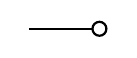
\begin{tikzpicture}
		\draw[thick,-o,black] (0.,0.) -- (1.0,0.);
		\end{tikzpicture}
	\end{textblock*}
	
	\begin{textblock*}{0.5\hsize}(#1+0.075\paperwidth,0.1\vsize)
		\normalsize
		\vspace{0.6mm}
		%		\centering
		#2
	\end{textblock*}
}

% new color for the bullet/subbullet
\newcommand{\mybullet}{$\textcolor{myblack}{\bullet}$}
\newcommand{\mysubbullet}{$\textcolor{myblack}{\circ}$}
\newcommand{\ev}{\mathbb{E}_{\text{p}(\bm x,y)}}
\newcommand{\pluseq}{\mathrel{+}=}

\newcommand{\beginbackup}{
   \newcounter{framenumbervorappendix}
   \setcounter{framenumbervorappendix}{\value{framenumber}}
}
\newcommand{\backupend}{
   \addtocounter{framenumbervorappendix}{-\value{framenumber}}
   \addtocounter{framenumber}{\value{framenumbervorappendix}} 
}

%----------------------------------------------------------------------------------------
%	TITLE PAGE
%----------------------------------------------------------------------------------------

\author[Sergey Korpachev]{Sergey Korpachev}%
%\author[Sergey Korpachev]{Sergey Korpachev\inst{1, 2} on behalf of Dépôt}%
\institute[]{
%\institute[MIPT, LPI]{
%	\newline
%	\inst{1} {Moscow Institute of Physics and Technology}\\
%	\vspace{1mm}
%	\inst{2} {Lebedev Physical Institute of the Russian Academy of Sciences}\\
}
%\titlegraphic{
%	%\vspace{-.5cm}
%	%\hspace{1cm}
%	
\includegraphics[width=2.5cm]{mipt_logo.png}\hspace*{0.1cm}
%	
\includegraphics[width=1.5cm]{images/newLogoLPI.png}\hspace*{0.6cm}
%}

\title[Machine Learning (GitHub: SergeyKorpachev)]{}
%\date[\today]{}
\date[March 23, 2023]{}

%------------------------------------------------

\begin{document}

\begin{frame}
\centering
\huge

%\vspace{-0.3\paperheight}
\begin{tcolorbox}[colframe=white, colback=mygrey, width=0.45\paperwidth,
	arc=2.mm, boxsep=2mm,
	box align=center,
	halign=center,
	valign=center,
	]
	\Large
	Machine Learning: short introduction (Trees and ANN)
\end{tcolorbox}

\vspace{0.1\paperheight}
\centering
\large
\insertauthor\\

\scriptsize
\vspace{0.03\paperheight}
\hspace{0.17\paperwidth}
\insertinstitute

\vfill
\inserttitlegraphic
\transfade[duration=.4]
\end{frame}

%%------------------------------------------------
%------------------------------------------------
\section{Outline}
%------------------------------------------------
%------------------------------------------------

\begin{frame}[t]
\myframetitle{0.2\paperwidth}{0.04\paperwidth}{\insertsection}

\vspace{0.25\paperheight}
\begin{itemize}
	\itemsep1.2ex
	\setbeamertemplate{items}{\mybullet}
	\item Machine learning (ML)
	\item Data
	\item Features in ML
	\item ML pipeline
	\item Linear model
	\item Decision tree
	\item Neural network
\end{itemize}

\transfade[duration=.4]
\end{frame}

%------------------------------------------------
%------------------------------------------------
\section{Machine learning}
%------------------------------------------------
%------------------------------------------------

\begin{frame}[plain]
\centering
\huge

%\begin{textblock*}{0.3\paperwidth}(0.25\paperwidth,0.3\paperheight)
\centering
\vspace{0.1\paperheight}
\begin{tcolorbox}[colframe=white, colback=mygrey, width=0.5\paperwidth,
	arc=2.mm, boxsep=2mm,
	box align=center,
	halign=center,
	valign=center,
	]
	\insertsection
\end{tcolorbox}

%\end{textblock*}

\transfade[duration=.4]
\end{frame}

%------------------------------------------------

\subsection{what is it?}
\begin{frame}

\myframetitle{0.35\paperwidth}{0.04\paperwidth}{\insertsection}
\myframesubtitle{0.37\paperwidth}{\insertsubsection}

\centering
\vspace{0.20\textheight}

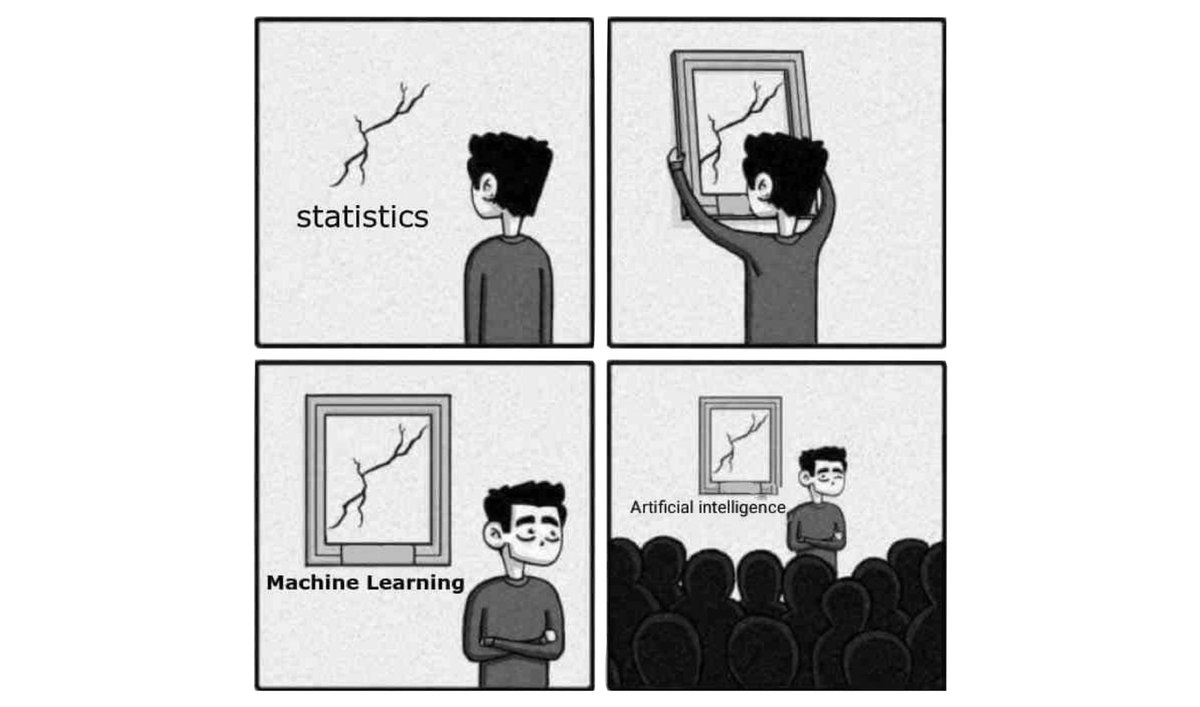
\includegraphics[width=0.4\textwidth]{what_is_ml.png}
\only<2->{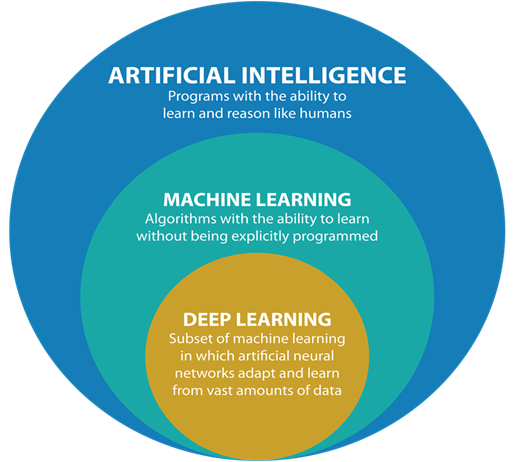
\includegraphics[width=0.27\textwidth]{ai_ml_dl.png}}
\hspace{0.07\textheight}
\only<3->{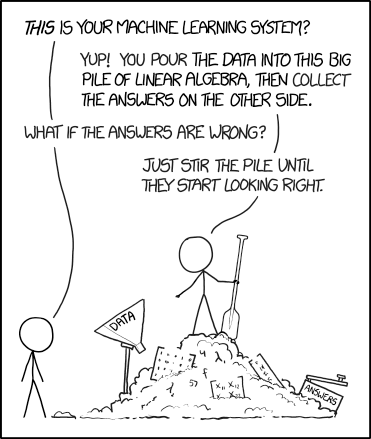
\includegraphics[width=0.25\textwidth]{approximation.png}}

\end{frame}

%------------------------------------------------

\subsection{The Fourth Paradigm (Tony Hey, ...)}
\begin{frame}
\myframetitle{0.35\paperwidth}{0.04\paperwidth}{\insertsection}
\myframesubtitle{0.37\paperwidth}{\insertsubsection}

\centering
\vspace{0.20\textheight}
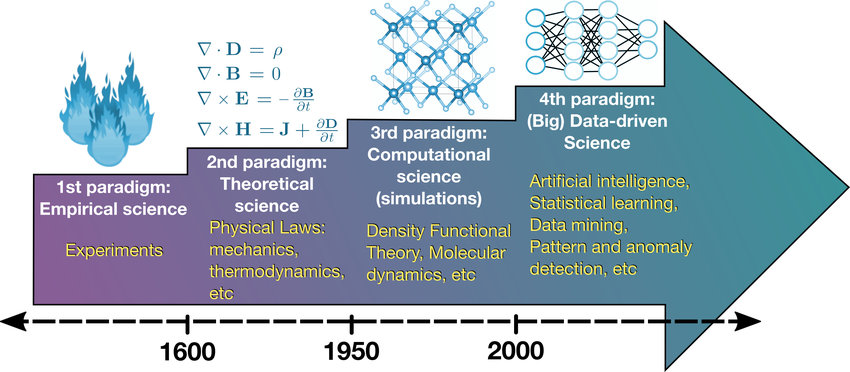
\includegraphics[width=1.0\textwidth]{science_paradigms.png}

\end{frame}

%------------------------------------------------
%------------------------------------------------
\section{Data}
%------------------------------------------------
%------------------------------------------------

\begin{frame}[plain]
\centering
\huge

%\begin{textblock*}{0.3\paperwidth}(0.25\paperwidth,0.3\paperheight)
\centering
\vspace{0.1\paperheight}
\begin{tcolorbox}[colframe=white, colback=mygrey, width=0.3\paperwidth,
	arc=2.mm, boxsep=2mm,
	box align=center,
	halign=center,
	valign=center,
	]
	\insertsection
\end{tcolorbox}

%\end{textblock*}

\transfade[duration=.4]
\end{frame}

%------------------------------------------------

\subsection{what is data?}
\begin{frame}

\myframetitle{0.27\paperwidth}{0.04\paperwidth}{\insertsection}
\myframesubtitle{0.29\paperwidth}{\insertsubsection}

\vspace{0.1\paperheight}
\begin{columns}
	\column{0.3\textwidth}
	Anything can be data:
	\begin{enumerate}
		\item Numbers
		\item Text
		\item Images
		\item Sound
		\item Geomap
		\item Particle collisions
		\item Knowledge
		\item You name it
	\end{enumerate}

	\column{0.7\textwidth}
	\begin{minipage}[c][.99\textheight][t]{\linewidth}
		\centering
		\vspace{0.2\paperheight}
		\begin{figure}[t]
			\centering
			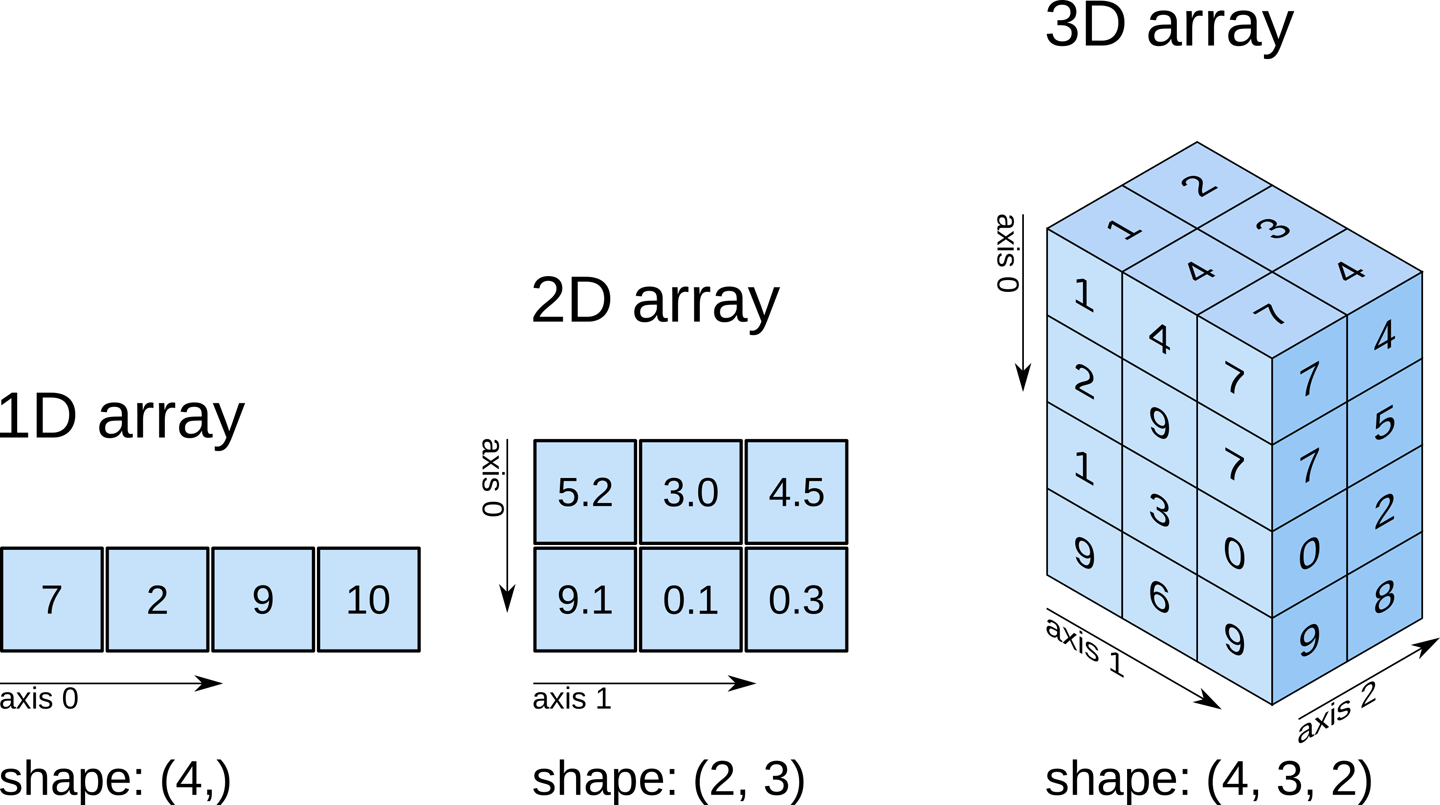
\includegraphics[width=0.4\linewidth]{numpy_array.png}
			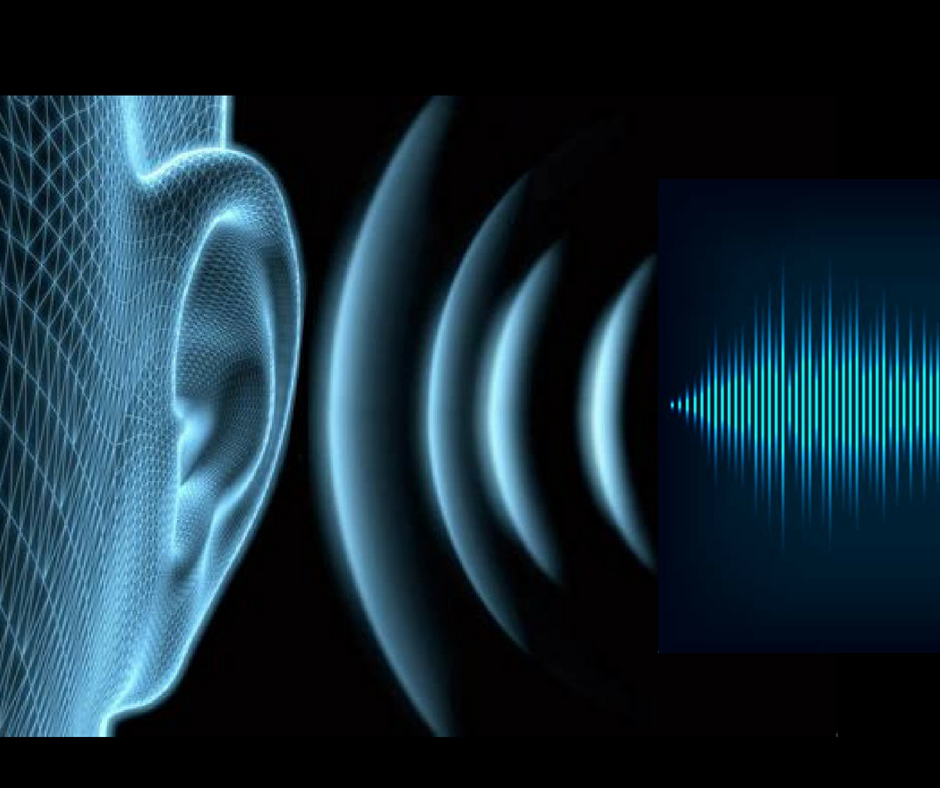
\includegraphics[width=0.25\linewidth]{sound}
			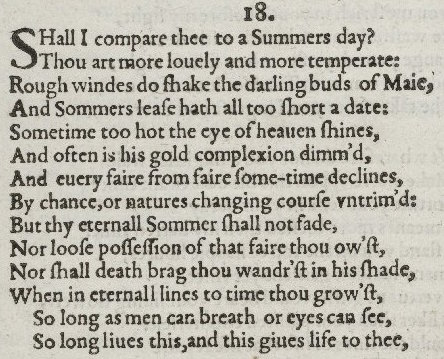
\includegraphics[width=0.2\linewidth]{Text}
			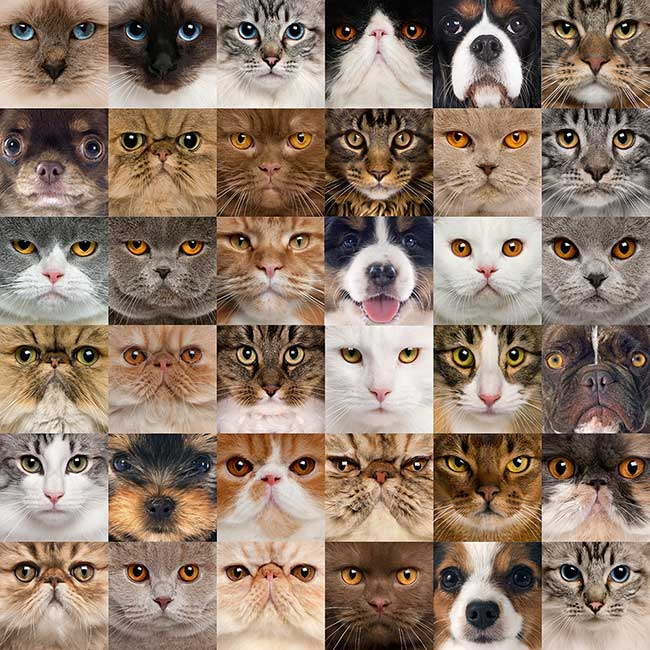
\includegraphics[width=0.25\linewidth]{cat}
			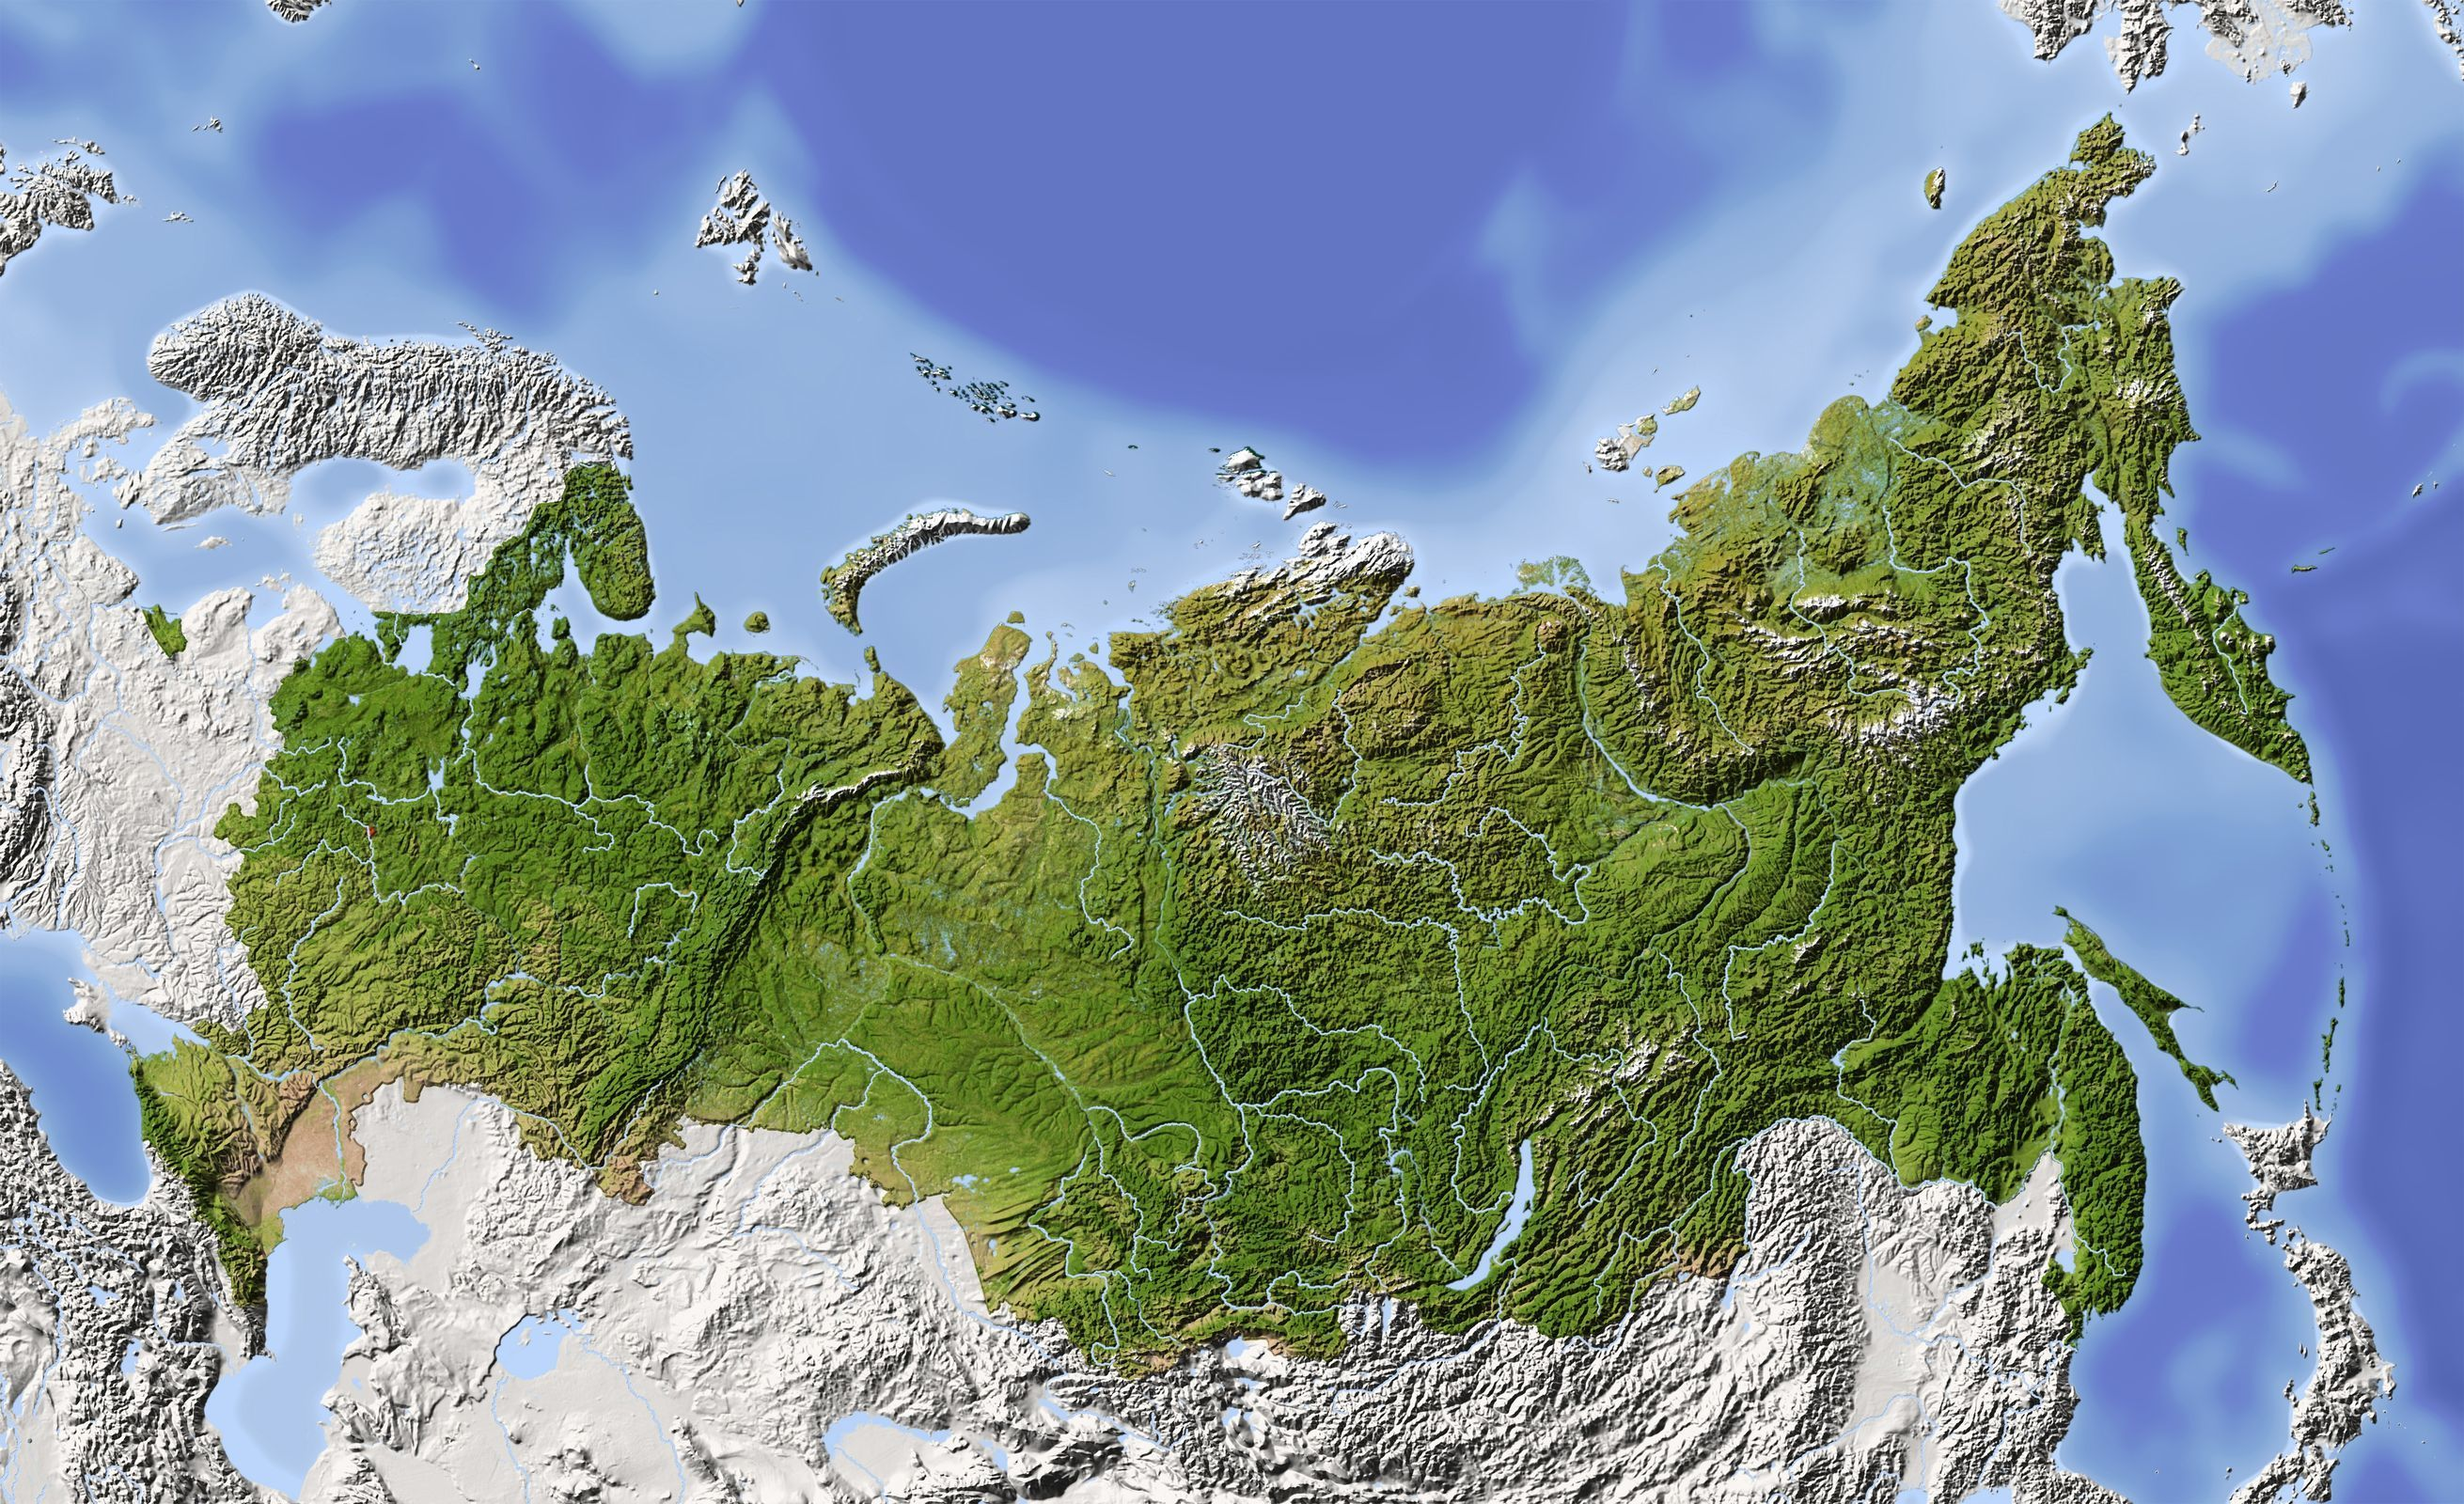
\includegraphics[width=0.3\linewidth]{geomap}
			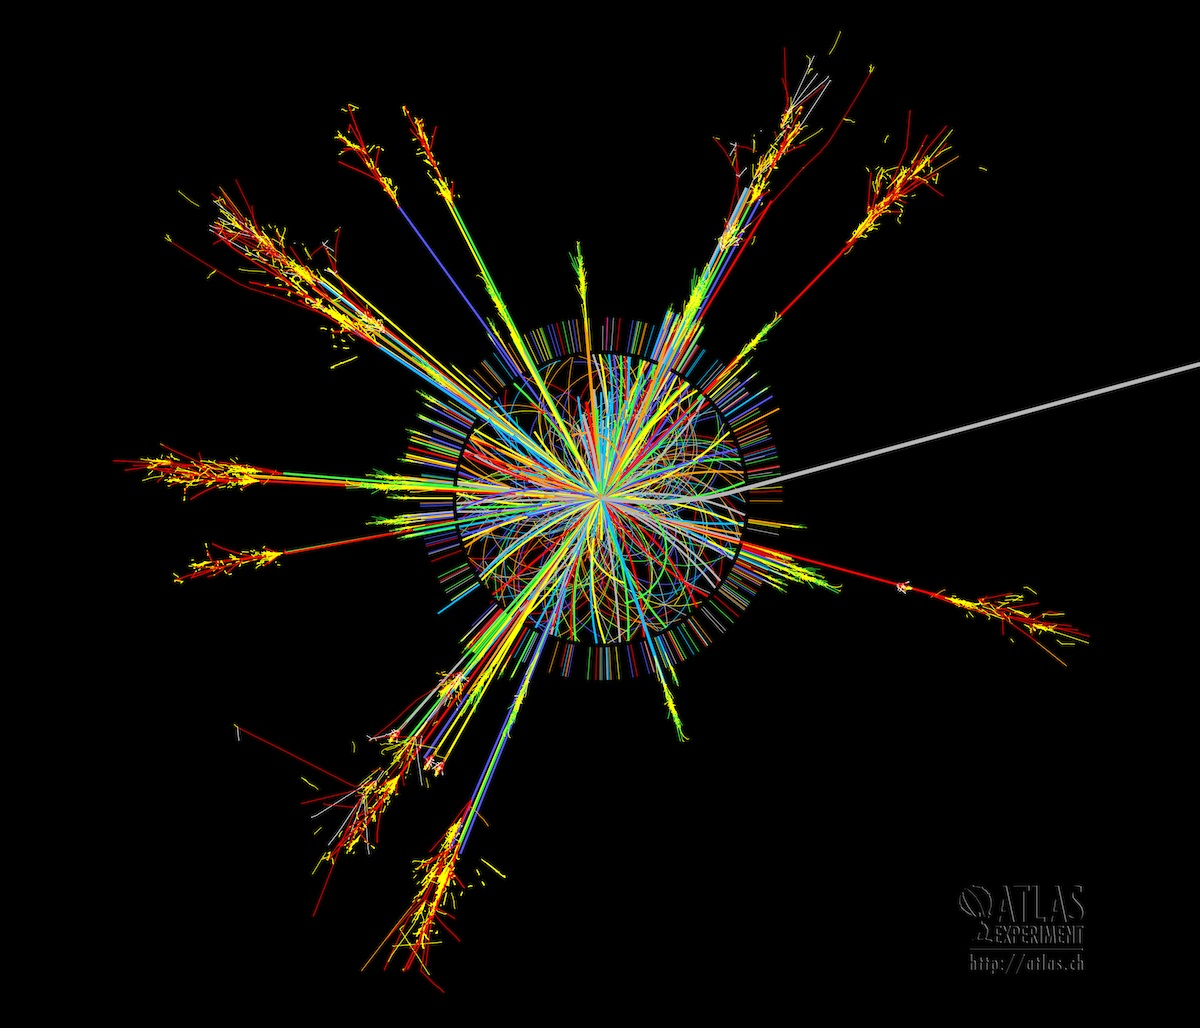
\includegraphics[width=0.3\linewidth]{HEP_event}
		\end{figure}	
	\end{minipage}
\end{columns}
\transfade[duration=.4]
\end{frame}

%------------------------------------------------
%------------------------------------------------
\section{Features in ML}
%------------------------------------------------
%------------------------------------------------

\begin{frame}[plain]
\centering
\huge

%\begin{textblock*}{0.3\paperwidth}(0.25\paperwidth,0.3\paperheight)
\centering
\vspace{0.1\paperheight}
\begin{tcolorbox}[colframe=white, colback=mygrey, width=0.4\paperwidth,
	arc=2.mm, boxsep=2mm,
	box align=center,
	halign=center,
	valign=center,
	]
	\insertsection
\end{tcolorbox}

%\end{textblock*}

\transfade[duration=.4]
\end{frame}

%------------------------------------------------

\subsection{not HEP}

\begin{frame}
\myframetitle{0.3\paperwidth}{0.04\paperwidth}{\insertsection}
\myframesubtitle{0.32\paperwidth}{\insertsubsection}

\centering
\vspace{0.2\paperheight}
\textbf{Supervised learning}
\vspace{0.05\paperheight}
\begin{columns}
	\column{0.5\textwidth}
	\centering
	\textbf{Classification}
	\begin{itemize}
		\setbeamertemplate{items}{\mybullet}
		\item cat, dog or muffin
		\item relevant or spam
		\item disease or not
        \item good or bad
        \item ...
	\end{itemize}
	
	\column{0.5\textwidth}
	\centering
	\textbf{Regression}
	\begin{itemize}
		\setbeamertemplate{items}{\mybullet}
		\item rent price
		\item temperature
		\item annual profit
        \item driving time
        \item ...
	\end{itemize}
\end{columns}

\vspace{0.1\paperheight}
Don't forget about \textbf{unsupervised learning}, \textbf{reinforcement learning}, \textbf{semi-supervised learning} and so on.

\end{frame}

%------------------------------------------------

\subsection{HEP}

\begin{frame}
\myframetitle{0.3\paperwidth}{0.04\paperwidth}{\insertsection}
\myframesubtitle{0.32\paperwidth}{\insertsubsection}

\centering
\vspace{0.2\paperheight}
\textbf{Supervised learning}
\vspace{0.05\paperheight}
\begin{columns}
	\column{0.5\textwidth}
	\centering
	\textbf{Classification}
	\begin{itemize}
		\setbeamertemplate{items}{\mybullet}
		\item b , c, uds jet
		\item $\pi$, K, $\mu$ particle
		\item t$\bar{\mathrm{t}}$ or QCD event
        \item select or reject trigger candidate
        \item ...
	\end{itemize}
	
	\column{0.5\textwidth}
	\centering
	\textbf{Regression}
	\begin{itemize}
		\setbeamertemplate{items}{\mybullet}
		\item energy resolution
		\item pile-up mitigation
        \item ...
	\end{itemize}
\end{columns}

\vspace{0.1\paperheight}
Don't forget about \textbf{unsupervised learning}, \textbf{reinforcement learning}, \textbf{semi-supervised learning} and so on.

\end{frame}

%------------------------------------------------

\subsection{ML challenges: slide 1 (A. Ustyuzhanin)}

\begin{frame}
\myframetitle{0.3\paperwidth}{0.04\paperwidth}{\insertsection}
\myframesubtitle{0.32\paperwidth}{\insertsubsection}

\centering
\vspace{0.2\paperheight}
\begin{itemize}
	\setbeamertemplate{items}{\mybullet}
	\item {Precise and fast particle tracking (single tracks, shower, jets)}
	\item {Particle identification}
	\item {Fast and accurate online data processing and filtering}
	\item {Anomaly detection (data quality monitoring, infrastructure monitoring)}
	\item {Detector design optimization (bayesian optimization, surrogate modelling)}
	\item {Data analysis (signal from background separation, ...)}
	\item {Simulation (speed-up simulation using generative models, simulator parameters optimization - tuning)}
	\item {...}
\end{itemize}

\end{frame}

%------------------------------------------------

\subsection{ML challenges: slide 2 (A. Ustyuzhanin)}

\begin{frame}
\myframetitle{0.3\paperwidth}{0.04\paperwidth}{\insertsection}
\myframesubtitle{0.32\paperwidth}{\insertsubsection}

\centering
\vspace{0.2\paperheight}
\begin{columns}
	\column{0.5\textwidth}
	\centering
	\textbf{Tracking system features}
	\begin{itemize}
		\setbeamertemplate{items}{\mybullet}
		\item Particle momentum
		\item Particle charge
		\item Track parameters
        \item Quality of track fit
        \item Number of track hits
        \item ...
	\end{itemize}
	
	\column{0.5\textwidth}
	\centering
	\textbf{RICH features}
	\begin{itemize}
		\setbeamertemplate{items}{\mybullet}
		\item Angle $\theta$
		\item Quality of angle reconstruction
		\item Reconstructed particle type
        \item Reconstructed particle energy
        \item Light intensity
        \item ...
	\end{itemize}
\end{columns}

\end{frame}

%------------------------------------------------

\subsection{ML challenges: slide 3 (A. Ustyuzhanin)}

\begin{frame}
\myframetitle{0.3\paperwidth}{0.04\paperwidth}{\insertsection}
\myframesubtitle{0.32\paperwidth}{\insertsubsection}

\centering
\vspace{0.2\paperheight}
\textbf{Calorimeter features}
\begin{itemize}
	\setbeamertemplate{items}{\mybullet}
	\item Measured particle energy
	\item Shower parameters: length, width, ...
	\item Number of clusters in each layer Intensity of the clusters
	\item Intensity of the clusters
    \item Distance form track of the original particle
    \item ...
\end{itemize}

\end{frame}

%------------------------------------------------

\subsection{ML challenges: slide 4 (A. Ustyuzhanin)}

\begin{frame}
\myframetitle{0.3\paperwidth}{0.04\paperwidth}{\insertsection}
\myframesubtitle{0.32\paperwidth}{\insertsubsection}

\centering
\vspace{0.2\paperheight}
\textbf{Muon detector features}
\begin{itemize}
	\setbeamertemplate{items}{\mybullet}
	\item Muon track parameters
	\item Quality of track fit
	\item Number of active layers
    \item Distance between the track and the active layers
    \item Length of shower
    \item ...
\end{itemize}

\end{frame}

%------------------------------------------------

\subsection{Example of my regression problem}

\begin{frame}
\myframetitle{0.3\paperwidth}{0.04\paperwidth}{\insertsection}
\myframesubtitle{0.32\paperwidth}{\insertsubsection}

\vspace{0.2\paperheight}
\begin{columns}
    \centering
	\column{0.5\textwidth}
	\begin{minipage}[t]{\linewidth}
	    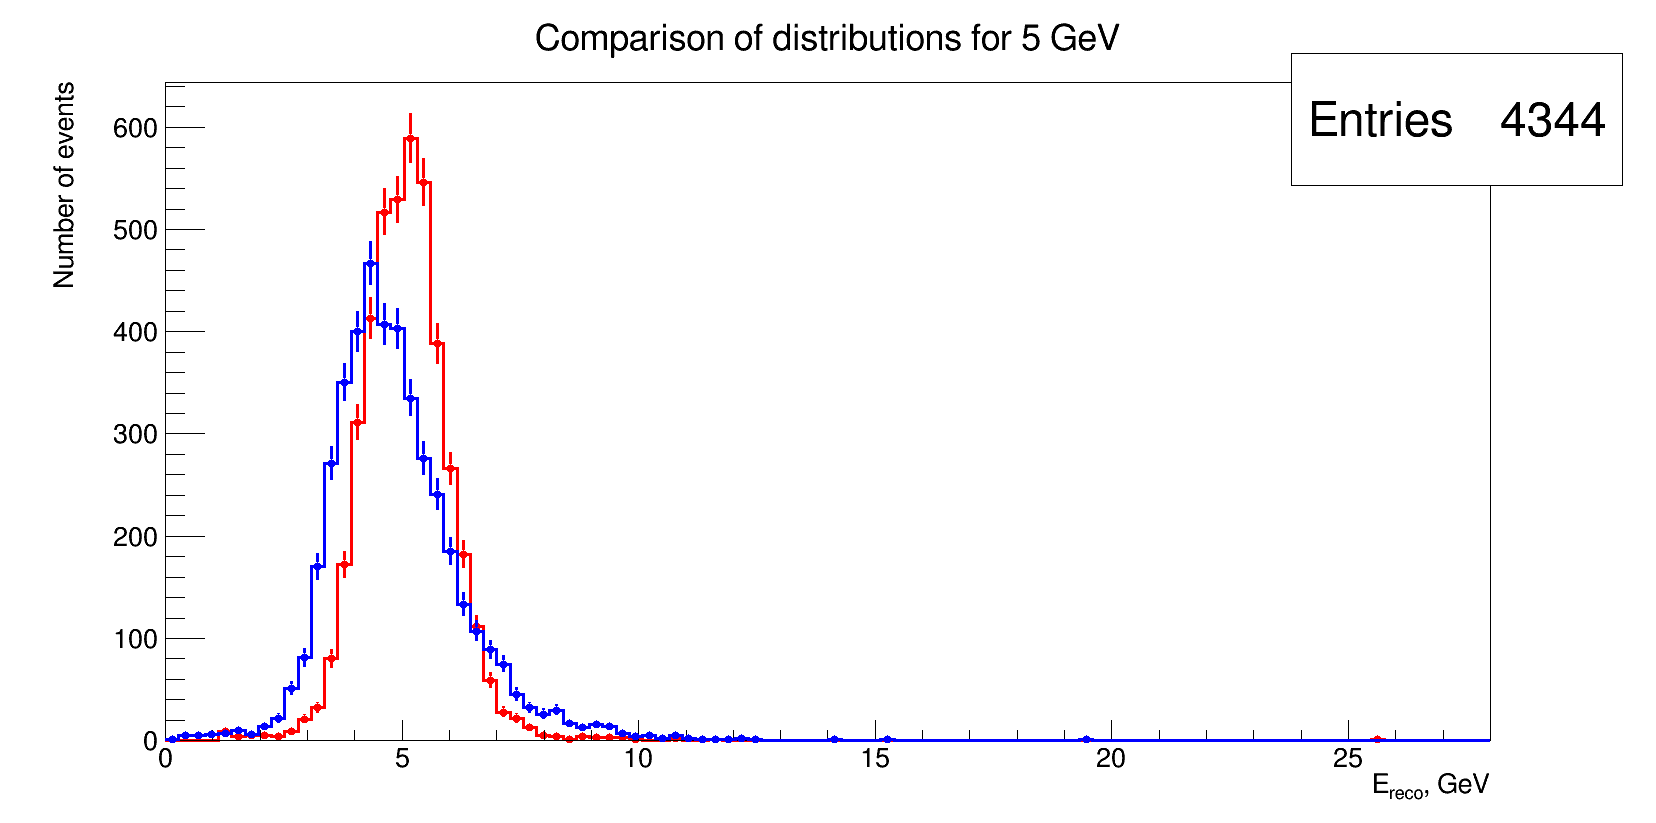
\includegraphics[width=1.0\linewidth]{comp_5.png}
    \end{minipage}%
    \column{0.5\textwidth}
    \begin{minipage}[t]{\linewidth}
        \centering
    	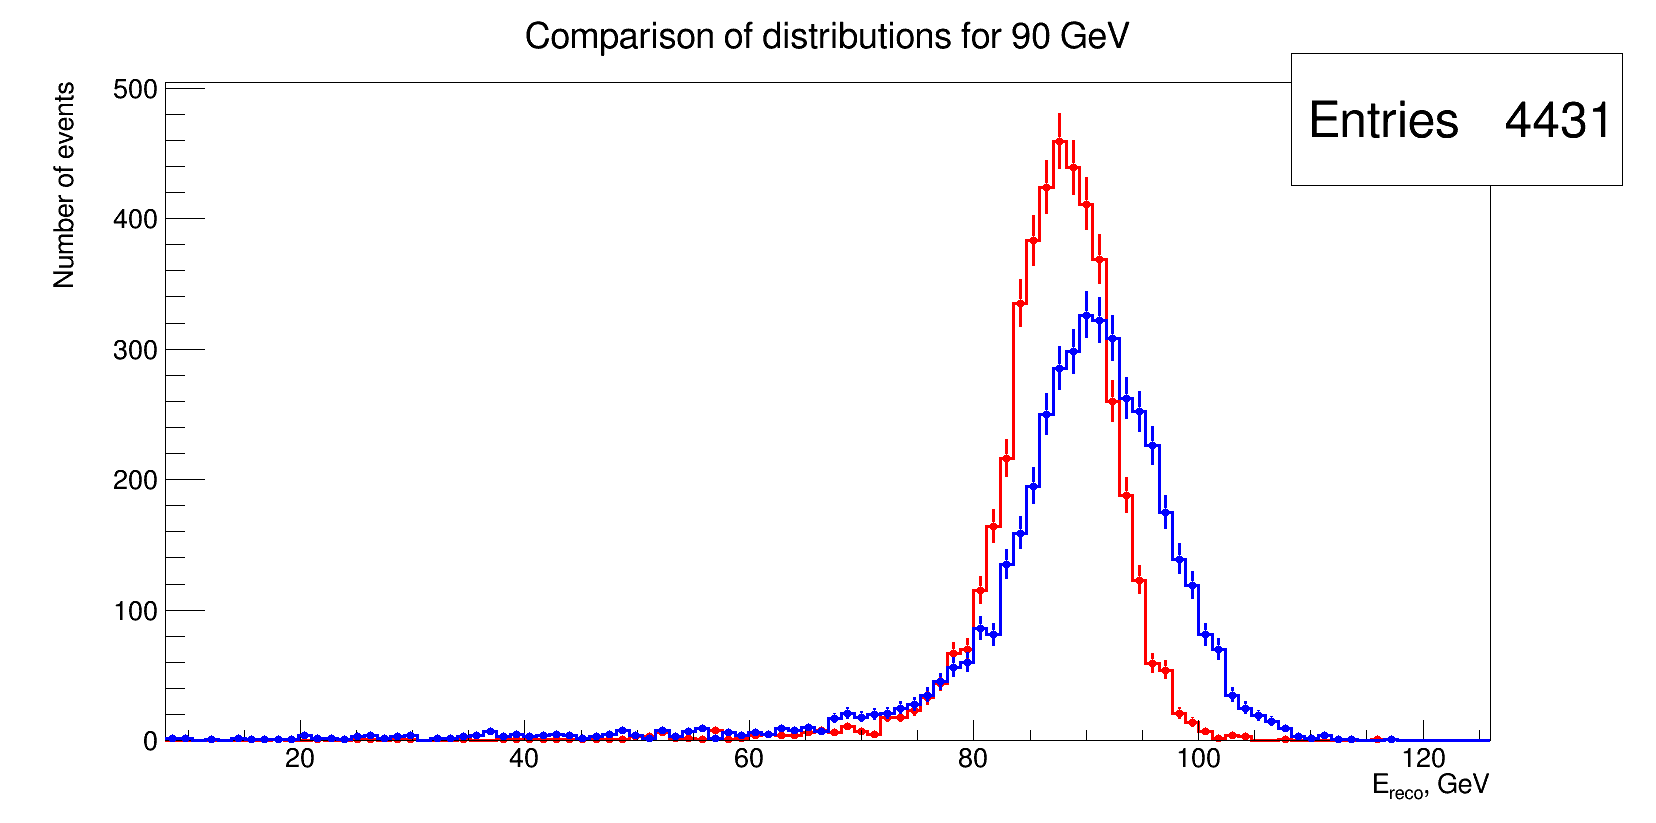
\includegraphics[width=1.0\linewidth]{comp_90.png}
    \end{minipage}
\end{columns}

\end{frame}

%------------------------------------------------

\subsection{SHAP value}

\begin{frame}
\myframetitle{0.3\paperwidth}{0.04\paperwidth}{\insertsection}
\myframesubtitle{0.32\paperwidth}{\insertsubsection}

\vspace{0.15\paperheight}
\centering
	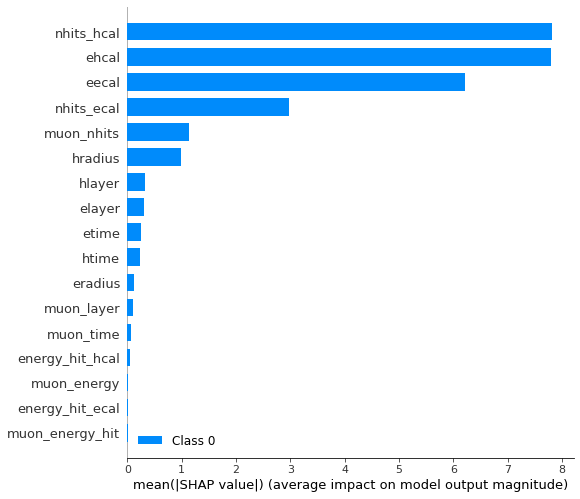
\includegraphics[width=0.55\linewidth]{shap_1.png}

\end{frame}

%------------------------------------------------
%------------------------------------------------
\section{ML pipeline}
%------------------------------------------------
%------------------------------------------------

\begin{frame}[plain]
\centering
\huge

%\begin{textblock*}{0.3\paperwidth}(0.25\paperwidth,0.3\paperheight)
\centering
\vspace{0.1\paperheight}
\begin{tcolorbox}[colframe=white, colback=mygrey, width=0.4\paperwidth,
	arc=2.mm, boxsep=2mm,
	box align=center,
	halign=center,
	valign=center,
	]
	\insertsection
\end{tcolorbox}

%\end{textblock*}

\transfade[duration=.4]
\end{frame}

%------------------------------------------------

\subsection{what is ML pipeline?}
\begin{frame}

\myframetitle{0.27\paperwidth}{0.04\paperwidth}{\insertsection}
\myframesubtitle{0.29\paperwidth}{\insertsubsection}

\vspace{0.1\paperheight}
\begin{minipage}[c][.99\textheight][t]{\linewidth}
		\centering
		\vspace{0.2\paperheight}
		\begin{figure}[t]
			\centering
			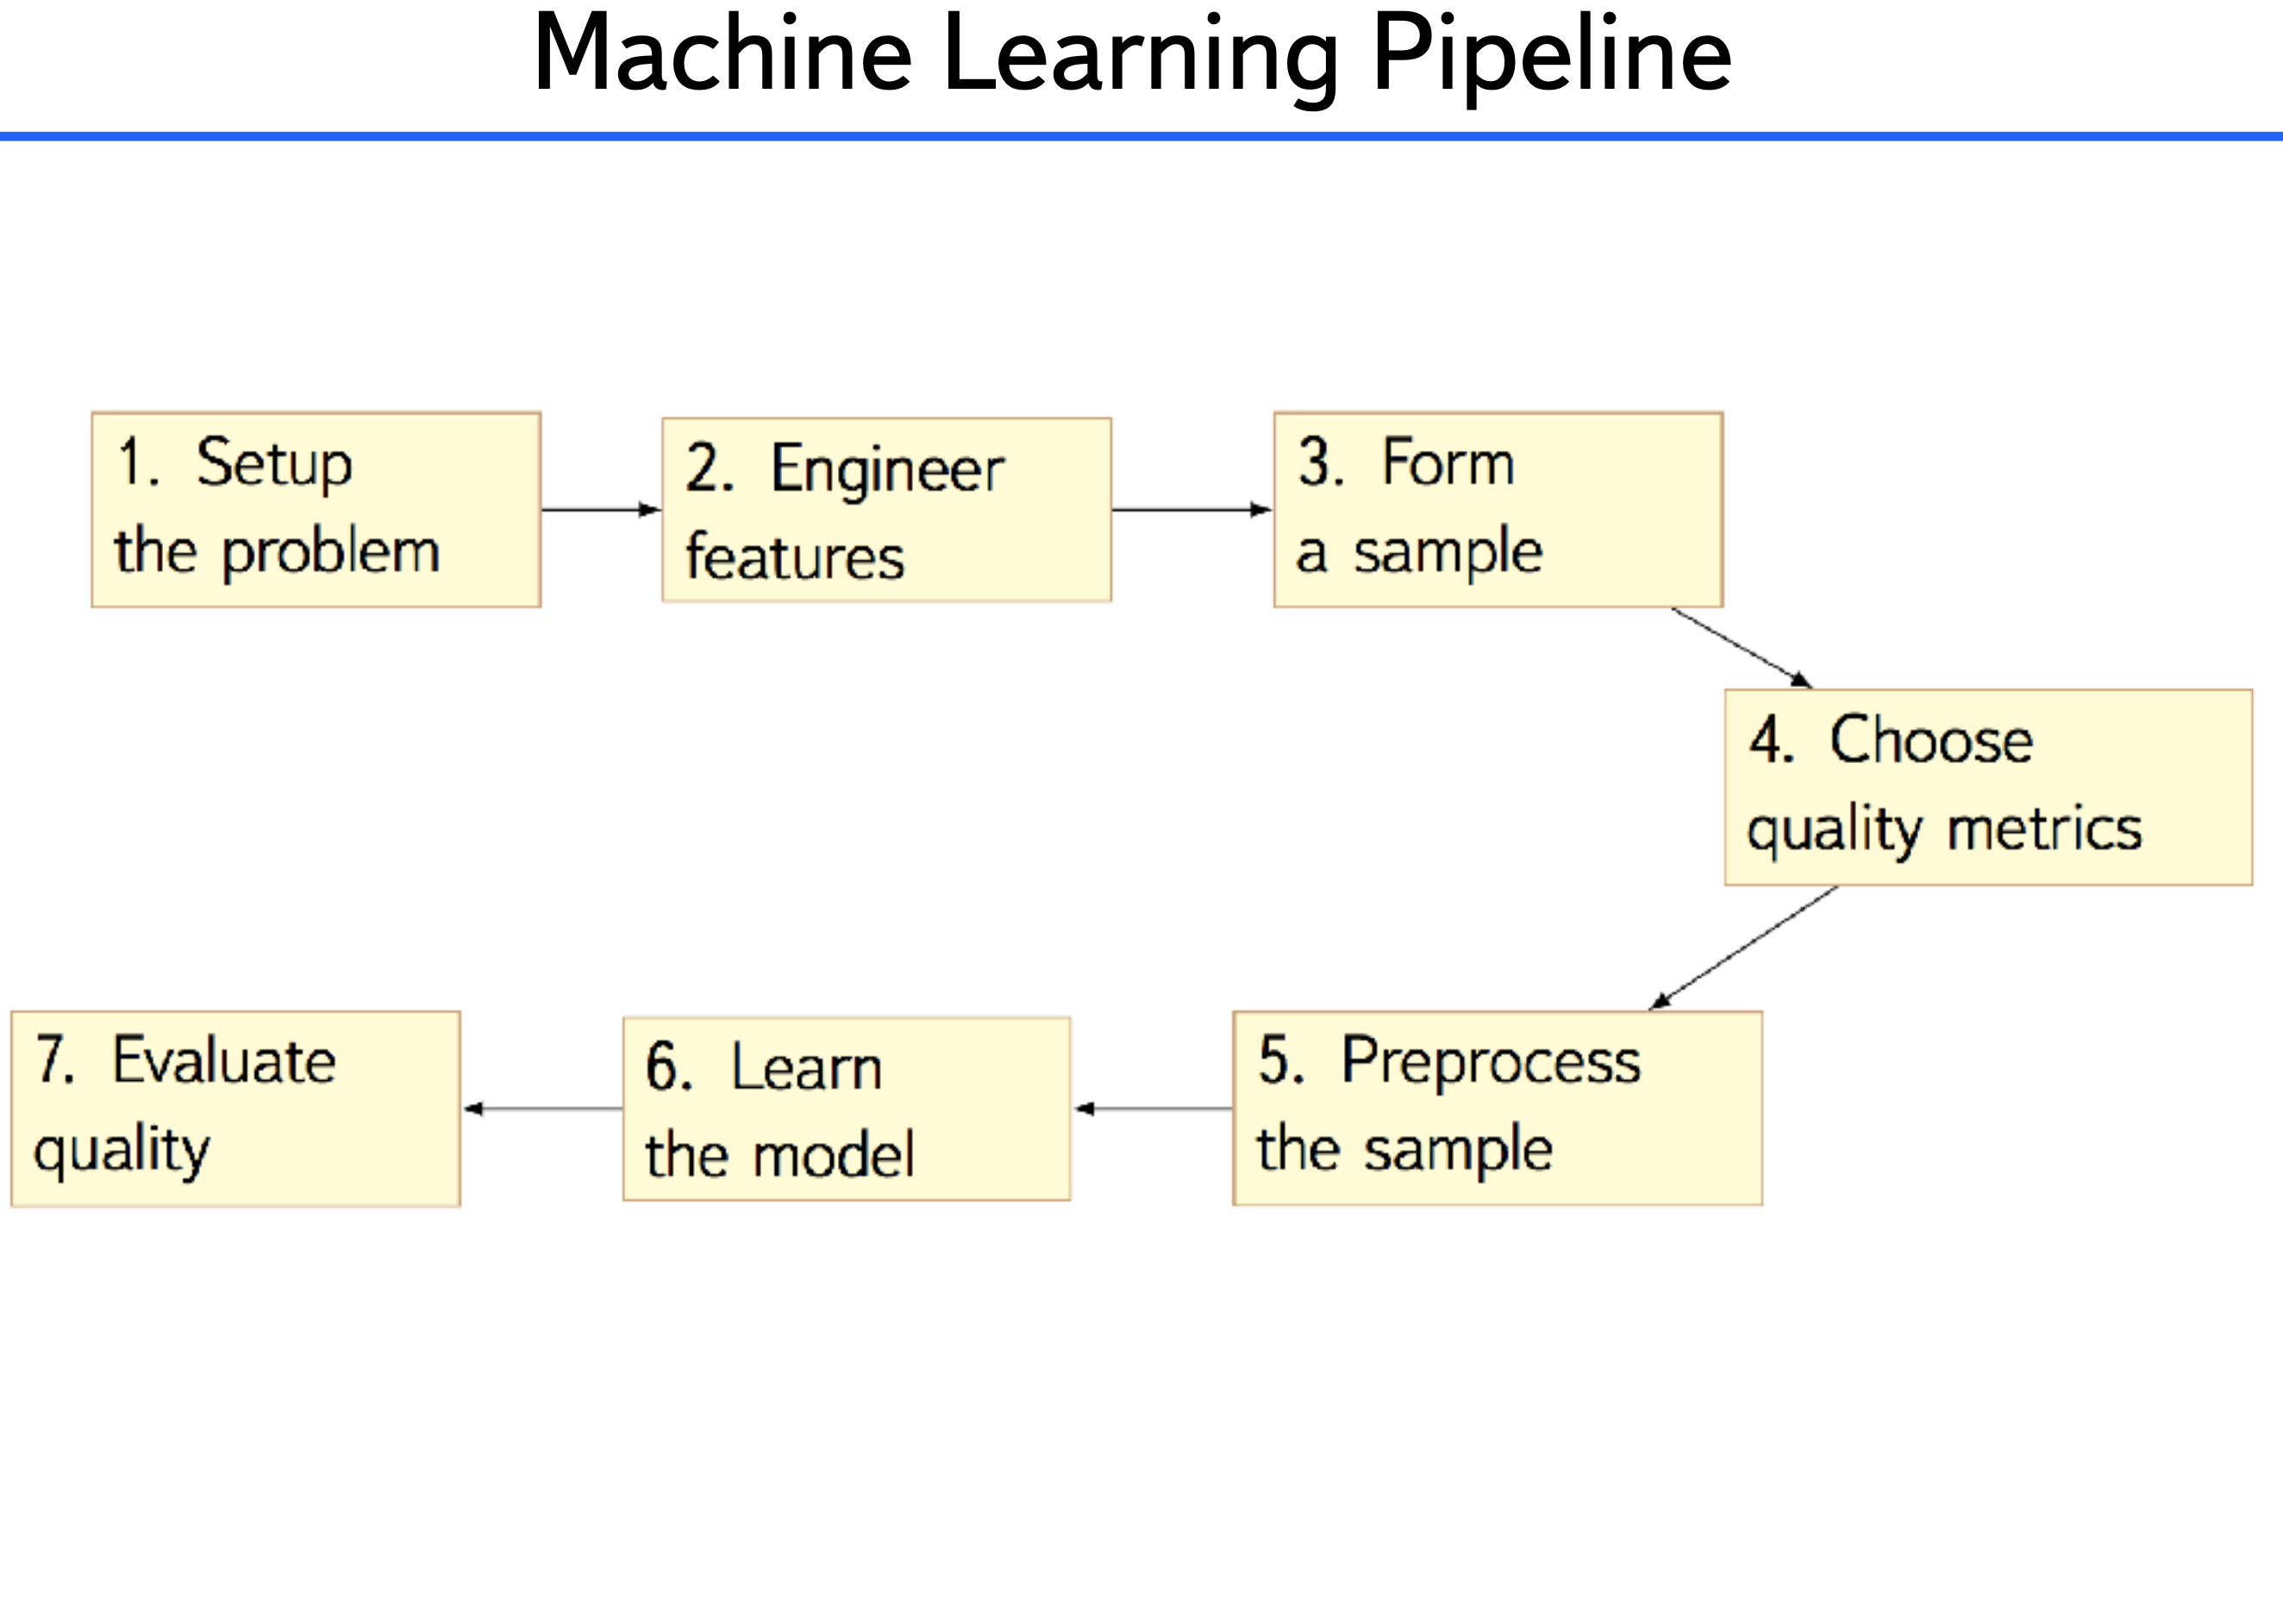
\includegraphics[width=0.448\linewidth]{pipeline1.png}
			\only<2->{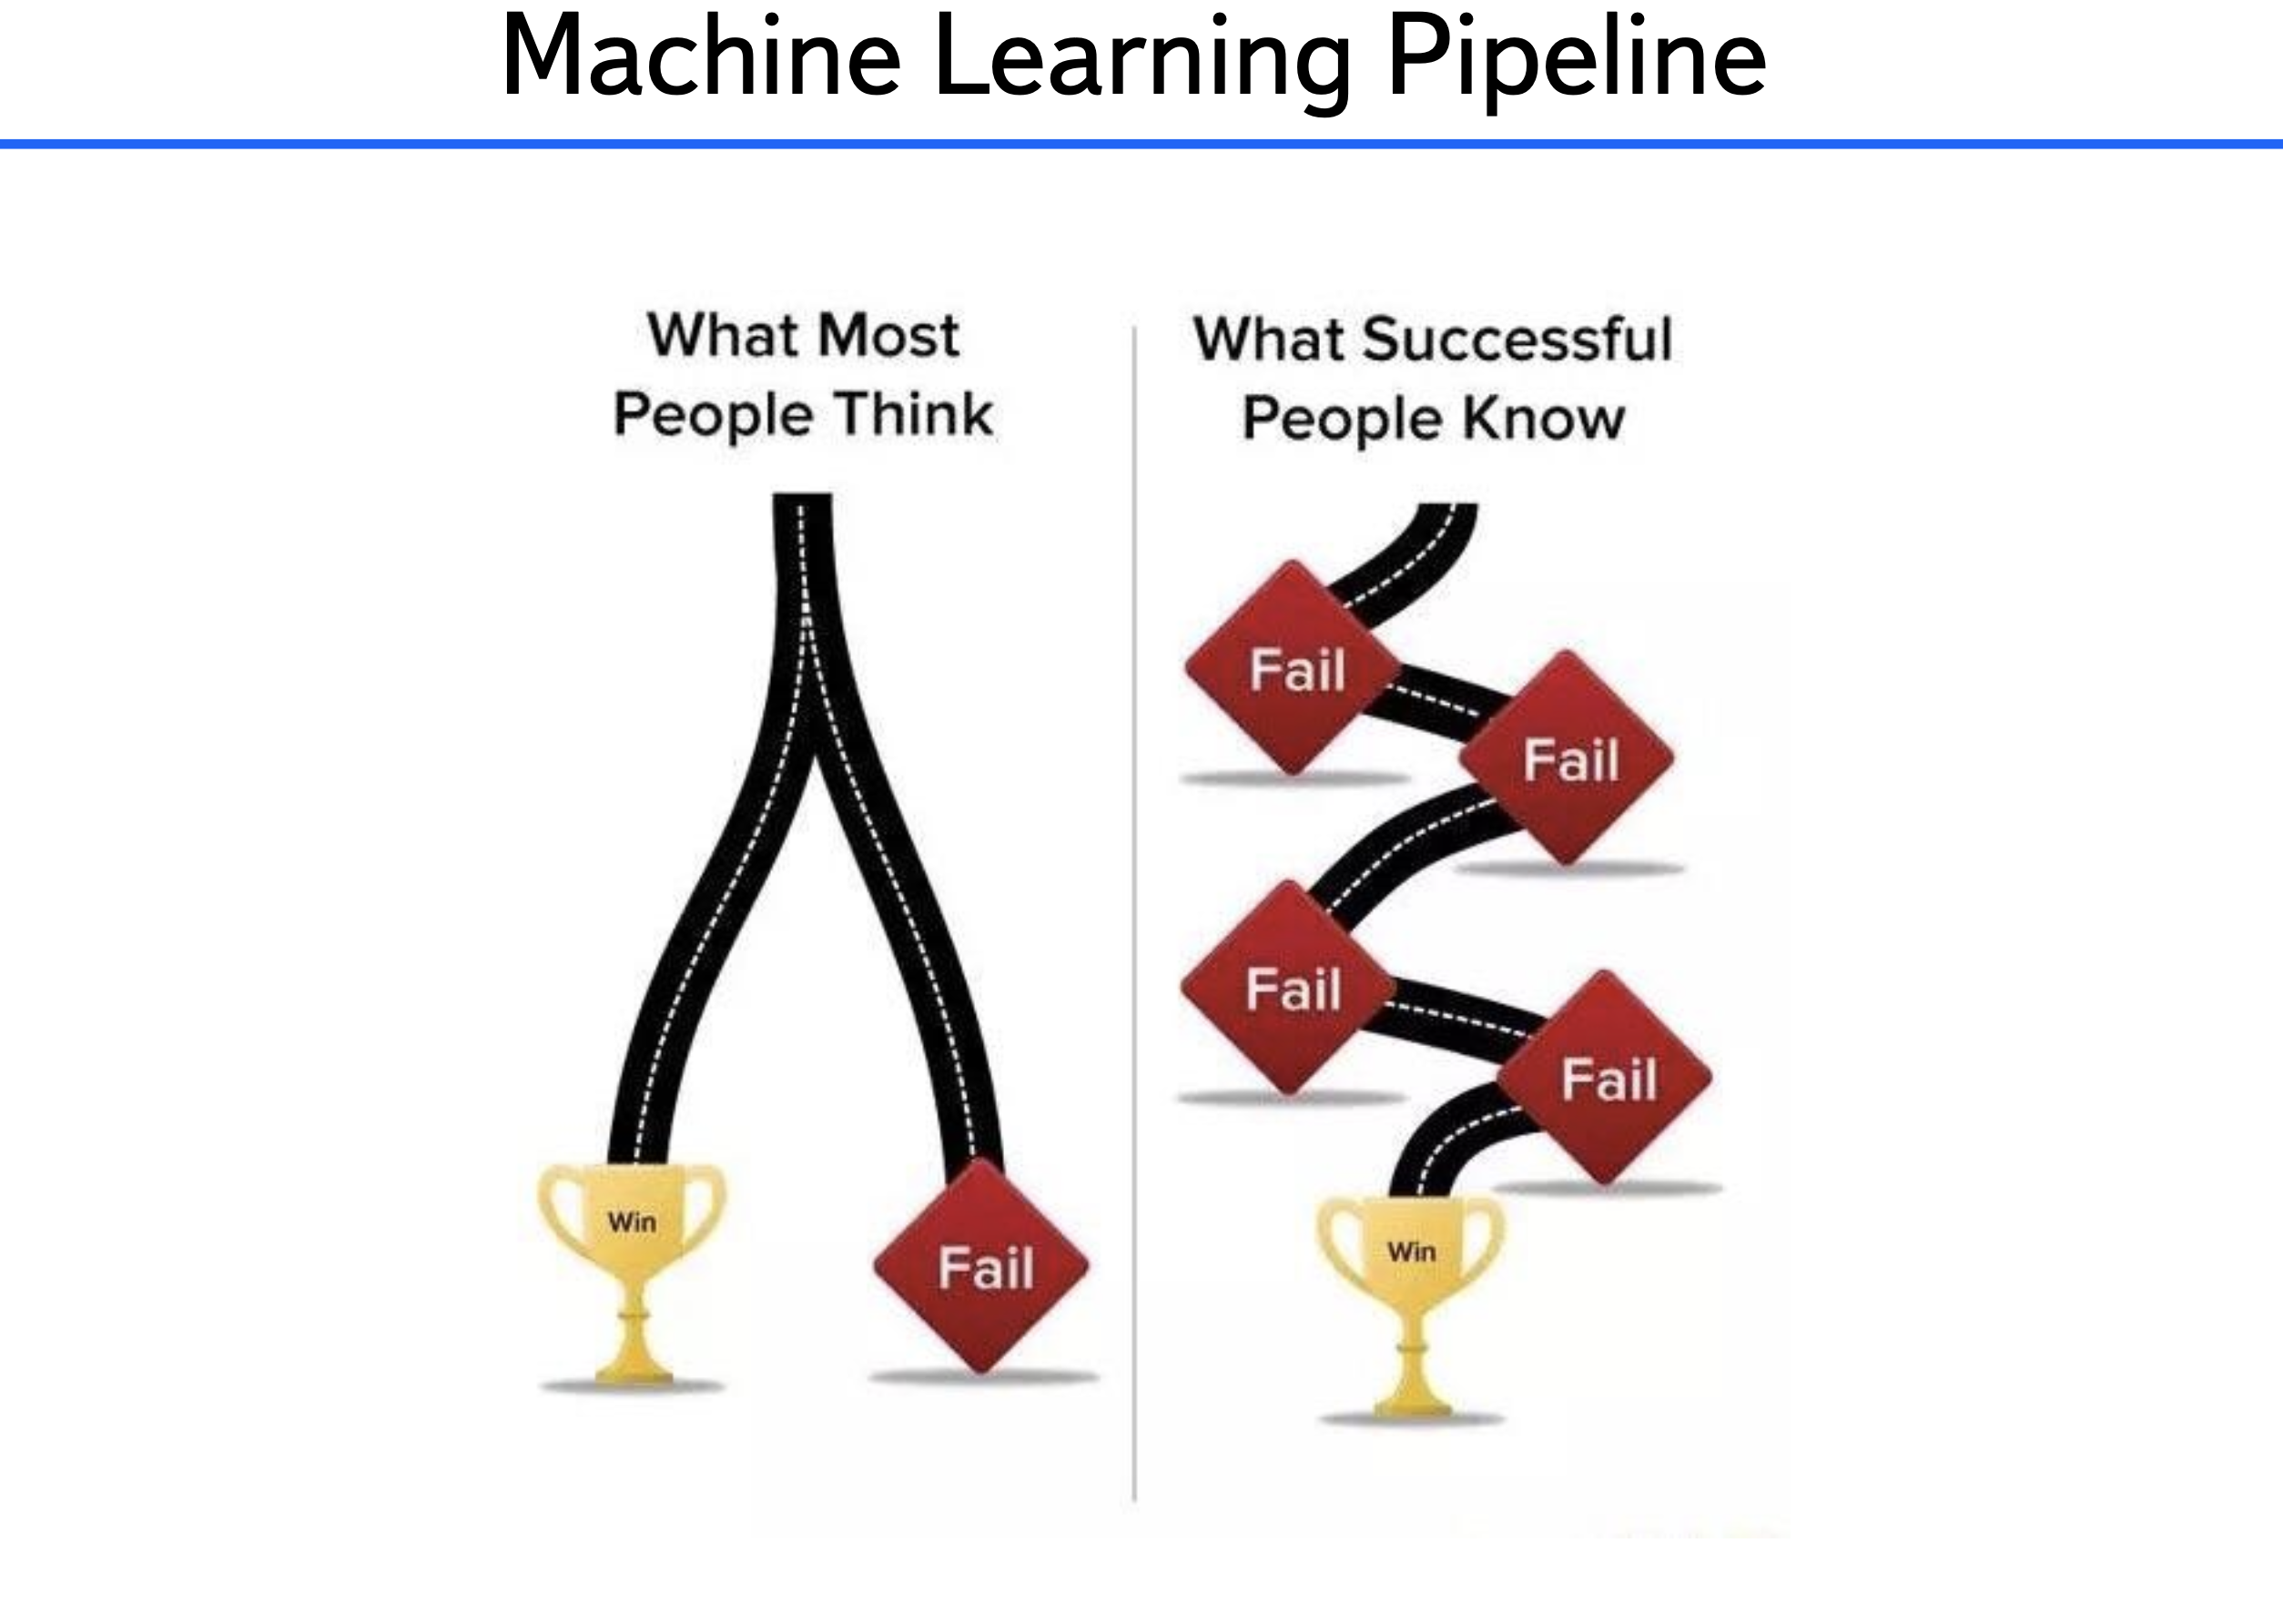
\includegraphics[width=0.45\linewidth]{pipeline2.png}}
		\end{figure}	
	\end{minipage}
\transfade[duration=.4]
\end{frame}

%------------------------------------------------
%------------------------------------------------
\section{Linear model}
%------------------------------------------------
%------------------------------------------------

\begin{frame}[plain]
\centering
\huge

%\begin{textblock*}{0.3\paperwidth}(0.25\paperwidth,0.3\paperheight)
\centering
\vspace{0.1\paperheight}
\begin{tcolorbox}[colframe=white, colback=mygrey, width=0.5\paperwidth,
	arc=2.mm, boxsep=2mm,
	box align=center,
	halign=center,
	valign=center,
	]
	\insertsection
\end{tcolorbox}

%\end{textblock*}

\transfade[duration=.4]
\end{frame}

%------------------------------------------------

\subsection{classification and regression}
\begin{frame}

\myframetitle{0.35\paperwidth}{0.04\paperwidth}{\insertsection}
\myframesubtitle{0.37\paperwidth}{\insertsubsection}

\vspace{0.2\paperheight}

\centering
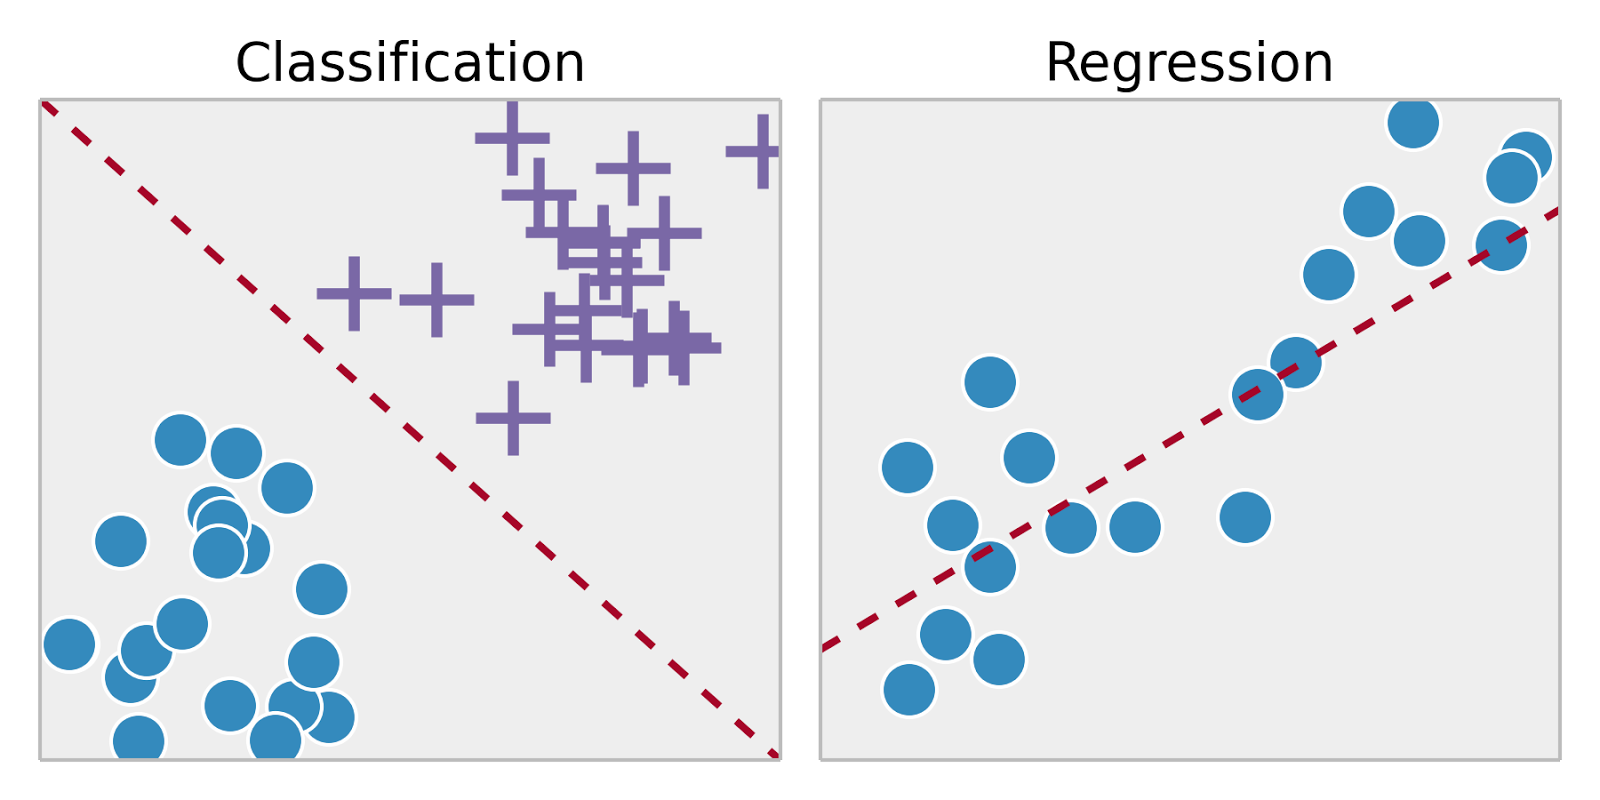
\includegraphics[width=0.8\textwidth]{linear_classification_regression.png}

\end{frame}

%------------------------------------------------

\subsection{regression}
\begin{frame}

\myframetitle{0.35\paperwidth}{0.04\paperwidth}{\insertsection}
\myframesubtitle{0.37\paperwidth}{\insertsubsection}

\vspace{0.2\paperheight}
\begin{columns}
	\column{0.55\textwidth}
	\begin{minipage}[t]{\linewidth}
		\begin{itemize}
			\item[\mybullet] $Y = \mathbb{R}$
			\item[\mybullet] N objects with K real features: $D = \mathbb{R}^K$
			\item[\mybullet] $a(\bm{x},\bm{\theta}) = \theta_0 + \sum\limits_{j=1}^{K}f_j(\bm{x})\cdot\theta_j $
			%\item[\mybullet] Extend and reassign:\\$[1, f_1(\bm{x}),\ldots ,f_K(\bm{x})] \equiv [1, x_1,\ldots ,x_K] \equiv \bm{x}$\\
			\item[\mybullet] Extend and reassign:\\$[1, f_1(\bm{x}),\ldots ,f_K(\bm{x})] \equiv \bm{x}$\\
			\vspace{0.3em}
			$[\theta_0, \ldots , \theta_K] \equiv \bm{\theta}$
			\item[\mybullet] Then $a(\bm{x},\bm{\theta}) = \langle\bm{x},\bm{\theta}\rangle$
		\end{itemize}
	\end{minipage}%	
	\column{0.5\textwidth}
	\begin{minipage}[c]{\linewidth}
		\centering
	
		\begin{itemize}
			\item[\mybullet] Minimization problem:
			\begin{itemize}
				\normalsize
				\item[\mysubbullet] $\mathcal{L}(\bm \theta) = \big(\langle\bm{x},\bm{\theta}\rangle - y\big)^2$
				\item[\mysubbullet] $Q(\bm{\theta}) = \frac{1}{N}\sum\limits_{i=1}^{N}\big(\langle\bm{x_i},\bm{\theta}\rangle - y_i\big)^2$
			\end{itemize}
			\item[\mybullet] Then we need to minimize $Q(\bm{\theta})$ by varying $\bm\theta$:
			\vspace{1mm}
			\begin{itemize}
				\normalsize
				\item[\mysubbullet] $\hat{a}=\text{arg}~ \underset{\bm{\theta} \in \Theta}{\text{min}}~Q(\bm{\theta})$
			\end{itemize}
			
		\end{itemize}	
	\end{minipage}
\end{columns}

\end{frame}

%------------------------------------------------

\subsection{classification}
\begin{frame}

\myframetitle{0.35\paperwidth}{0.04\paperwidth}{\insertsection}
\myframesubtitle{0.37\paperwidth}{\insertsubsection}

\vspace{0.2\paperheight}
\begin{columns}
	\column{0.55\textwidth}
	\begin{minipage}[t]{\linewidth}
		\begin{itemize}
			\item[\mybullet] $Y = \{-1, +1\}$
			\item[\mybullet] N objects with K real features: $D = \mathbb{R}^K$
			\item[\mybullet] $a(\bm{x},\bm{\theta}) = \theta_0 + \sum\limits_{j=1}^{K}f_j(\bm{x})\cdot\theta_j $
			\item[\mybullet] Extend and reassign:\\$[1, f_1(\bm{x}),\ldots ,f_K(\bm{x})] \equiv [1, x_1,\ldots ,x_K] \equiv \bm{x}$\\
			$[\theta_0, \ldots , \theta_K] \equiv \bm{\theta}$
			\item[\mybullet] Then $a(\bm{x},\bm{\theta}) = \langle\bm{x},\bm{\theta}\rangle$
		\end{itemize}
	\end{minipage}%	
	\column{0.5\textwidth}
	\begin{minipage}[c]{\linewidth}
		\centering
		
		\begin{itemize}
			\item[\mybullet] Minimization problem:
			\begin{itemize}
				\normalsize
				\item[\mysubbullet] $\mathcal{L}(\bm \theta) = \bigl[\text{sign}\langle\bm{x},\bm{\theta}\rangle \neq y\bigr]$
				\item[\mysubbullet] $Q(\bm{\theta}) = \frac{1}{N}\sum\limits_{i=1}^{N}\bigl[\text{sign}\langle\bm{x_i},\bm{\theta}\rangle \neq y_i\bigr]$
			\end{itemize}
			\item[\mybullet] Then we need to minimize $Q(\bm{\theta})$ by varying $\bm\theta$:
			\vspace{1mm}
			\begin{itemize}
				\normalsize
				\item[\mysubbullet] $\hat{a}=\text{arg}~ \underset{\bm{\theta} \in \Theta}{\text{min}}~Q(\bm{\theta})$
			\end{itemize}
			
		\end{itemize}	
	\end{minipage}
\end{columns}

\end{frame}

%------------------------------------------------
%------------------------------------------------
\section{Decision tree}
%------------------------------------------------
%------------------------------------------------

\begin{frame}[plain]
\centering
\huge

%\begin{textblock*}{0.3\paperwidth}(0.25\paperwidth,0.3\paperheight)
\centering
\vspace{0.1\paperheight}
\begin{tcolorbox}[colframe=white, colback=mygrey, width=0.4\paperwidth,
	arc=2.mm, boxsep=2mm,
	box align=center,
	halign=center,
	valign=center,
	]
	\insertsection
\end{tcolorbox}

%\end{textblock*}

\transfade[duration=.4]
\end{frame}

%------------------------------------------------

\subsection{motivation}
\begin{frame}

\myframetitle{0.27\paperwidth}{0.04\paperwidth}{\insertsection}
\myframesubtitle{0.29\paperwidth}{\insertsubsection}

\centering
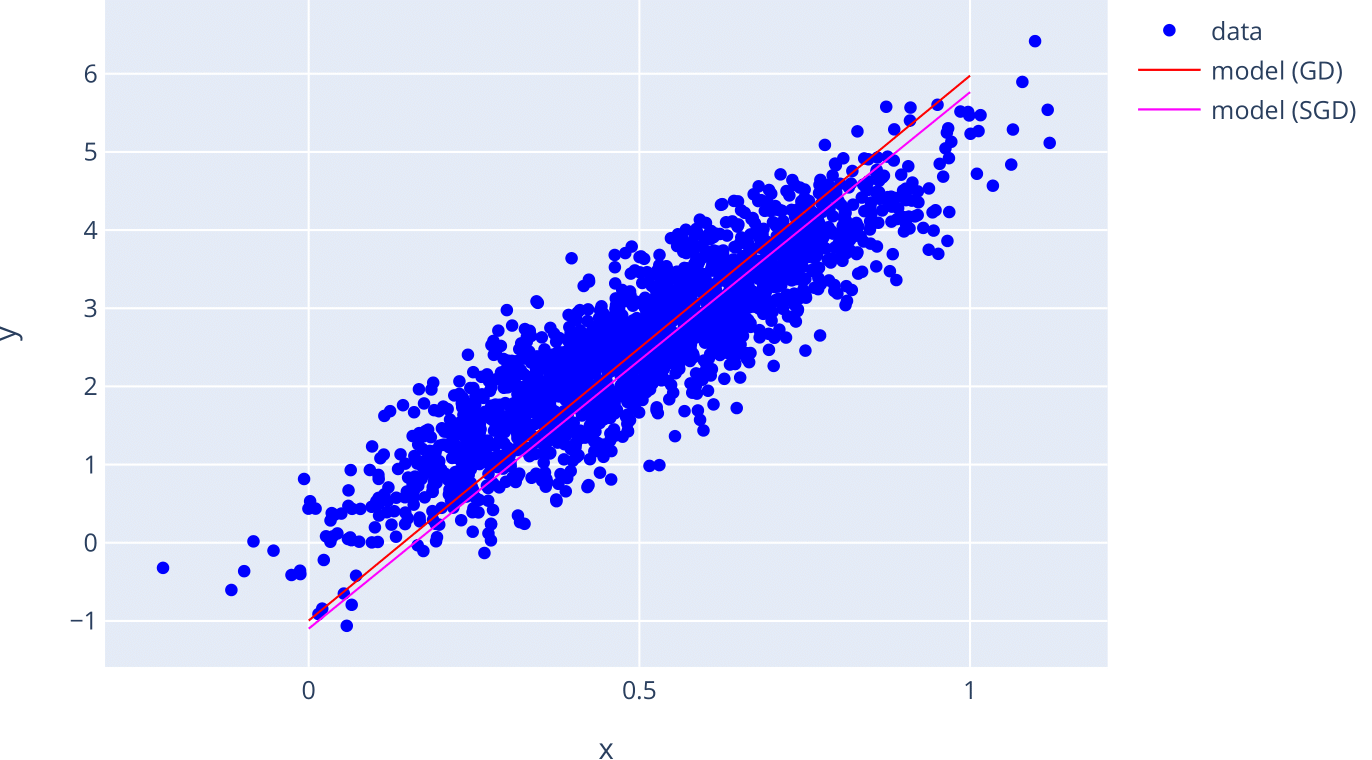
\includegraphics[width=0.3\textwidth]{data+fit.png}
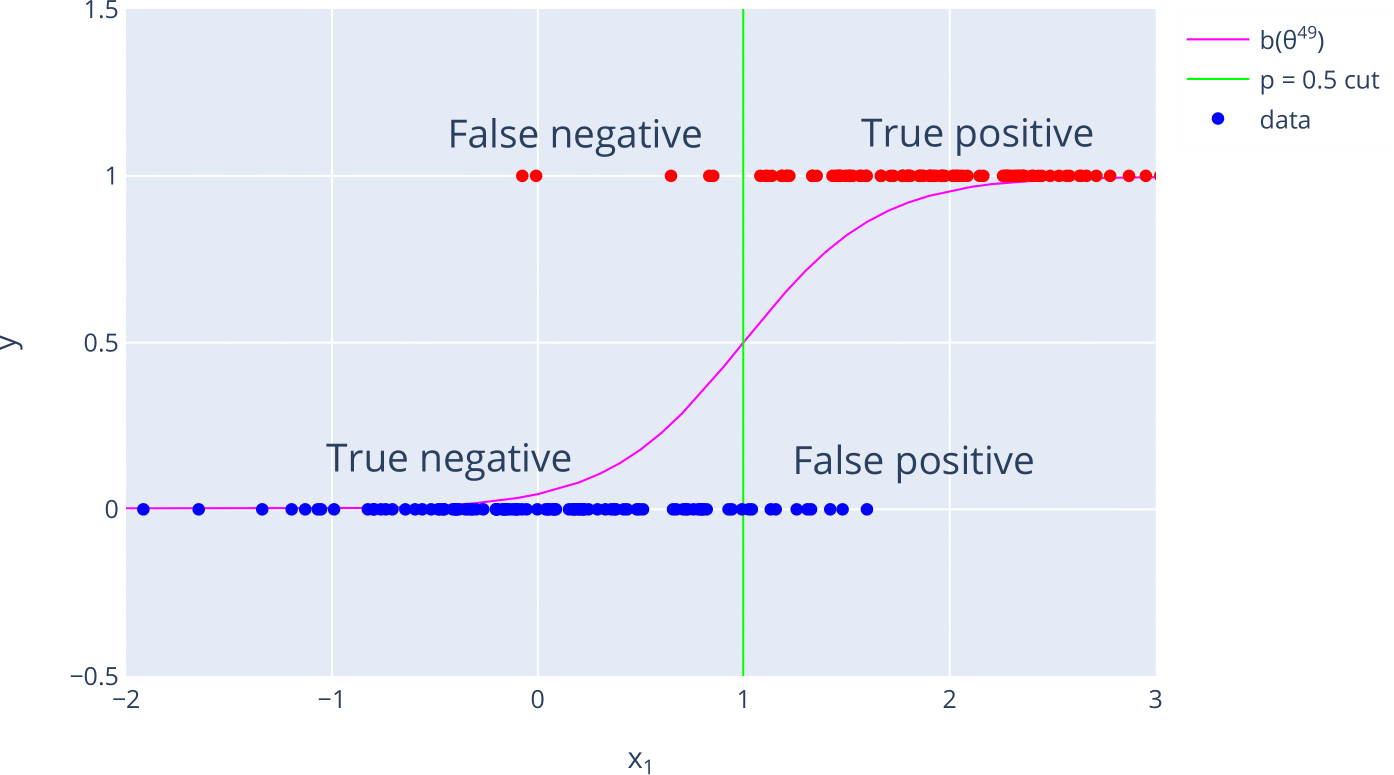
\includegraphics[width=0.3\textwidth]{class_confusions.png}
\only<2->{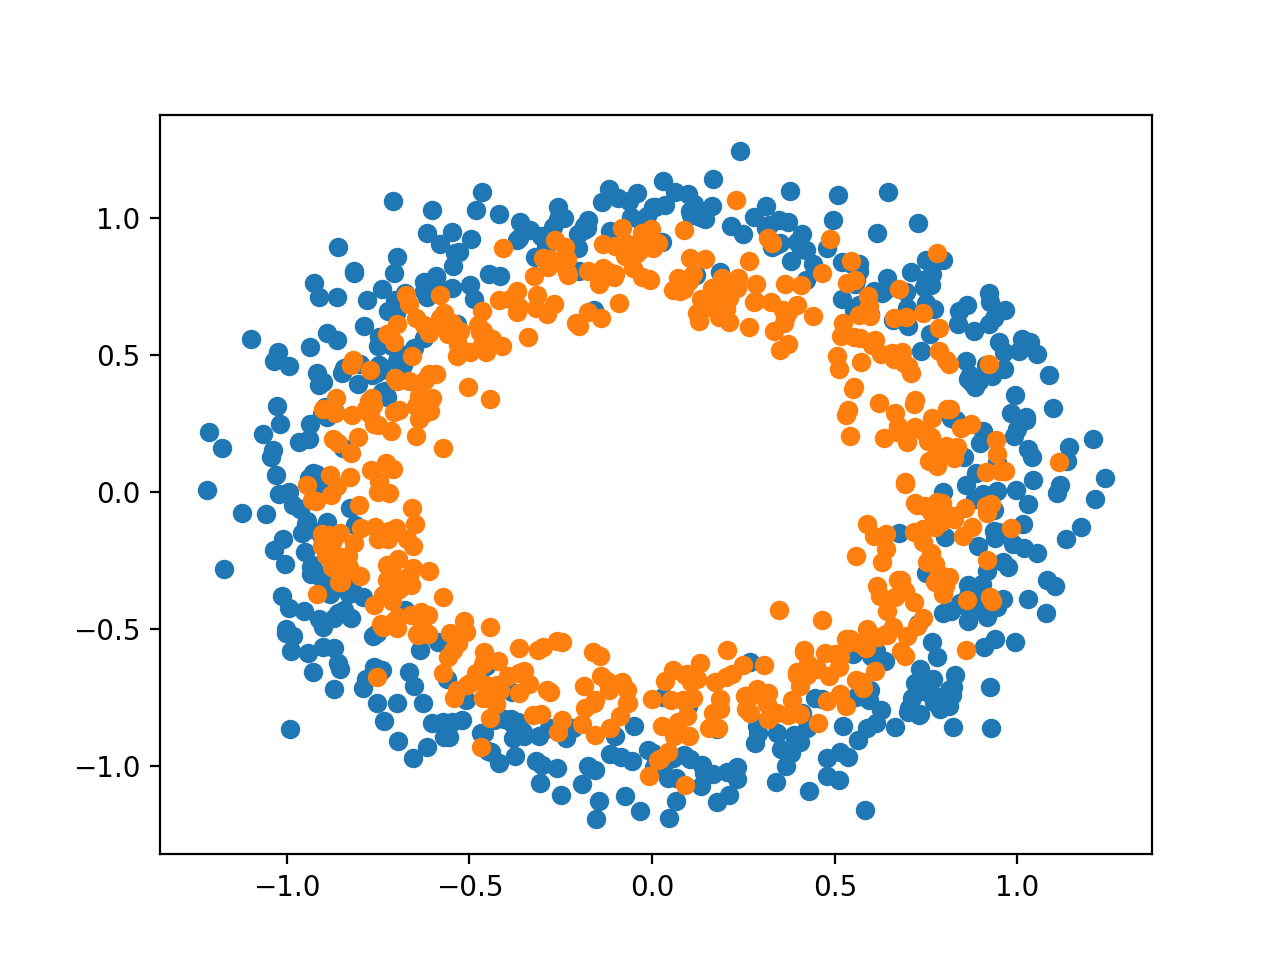
\includegraphics[width=0.25\textwidth]{circles}}

\begin{textblock*}{0.9\paperwidth}(0.05\paperwidth, 0.6\paperheight)
\begin{itemize}
	\itemsep0.8ex
	\footnotesize
	\setbeamertemplate{items}{\mybullet}
	\item In the previous part we explored linear models:
	\begin{itemize}
		\footnotesize
		\setbeamertemplate{items}{\textcolor{Gray}{\MVRightArrow}}
		\item nicely describe linear correlations
		\item fast and easy to train
%		\item performing well with large number of samples/features
	\end{itemize}
	\item<2-> However, they are poor in modelling non-linearities
	\item<2-> Additional heuristics might be applied (e.g. polynomial features) but are ad-hoc
\end{itemize}

\begin{textblock*}{0.3\paperwidth}(0.67\paperwidth, 0.7\paperheight)
	\footnotesize
	\only<3->{\centering \textcolor{myorange}{Is there a more general way to describe non-linearities?}}
\end{textblock*}	

\end{textblock*}
\end{frame}

%------------------------------------------------

\begin{frame}\myframetitle{0.27\paperwidth}{0.04\paperwidth}{\insertsection}
\myframesubtitle{0.29\paperwidth}{\insertsubsection}
\vspace{0.25\textheight}
\begin{itemize}
    \item[\mybullet]  What is the simplest way to approximate a function?
    \item[\mybullet] Using \textbf{piecewise linear function}
\end{itemize}
   \begin{columns}
   \column{0.5\linewidth}
    \begin{figure}
        \centering
        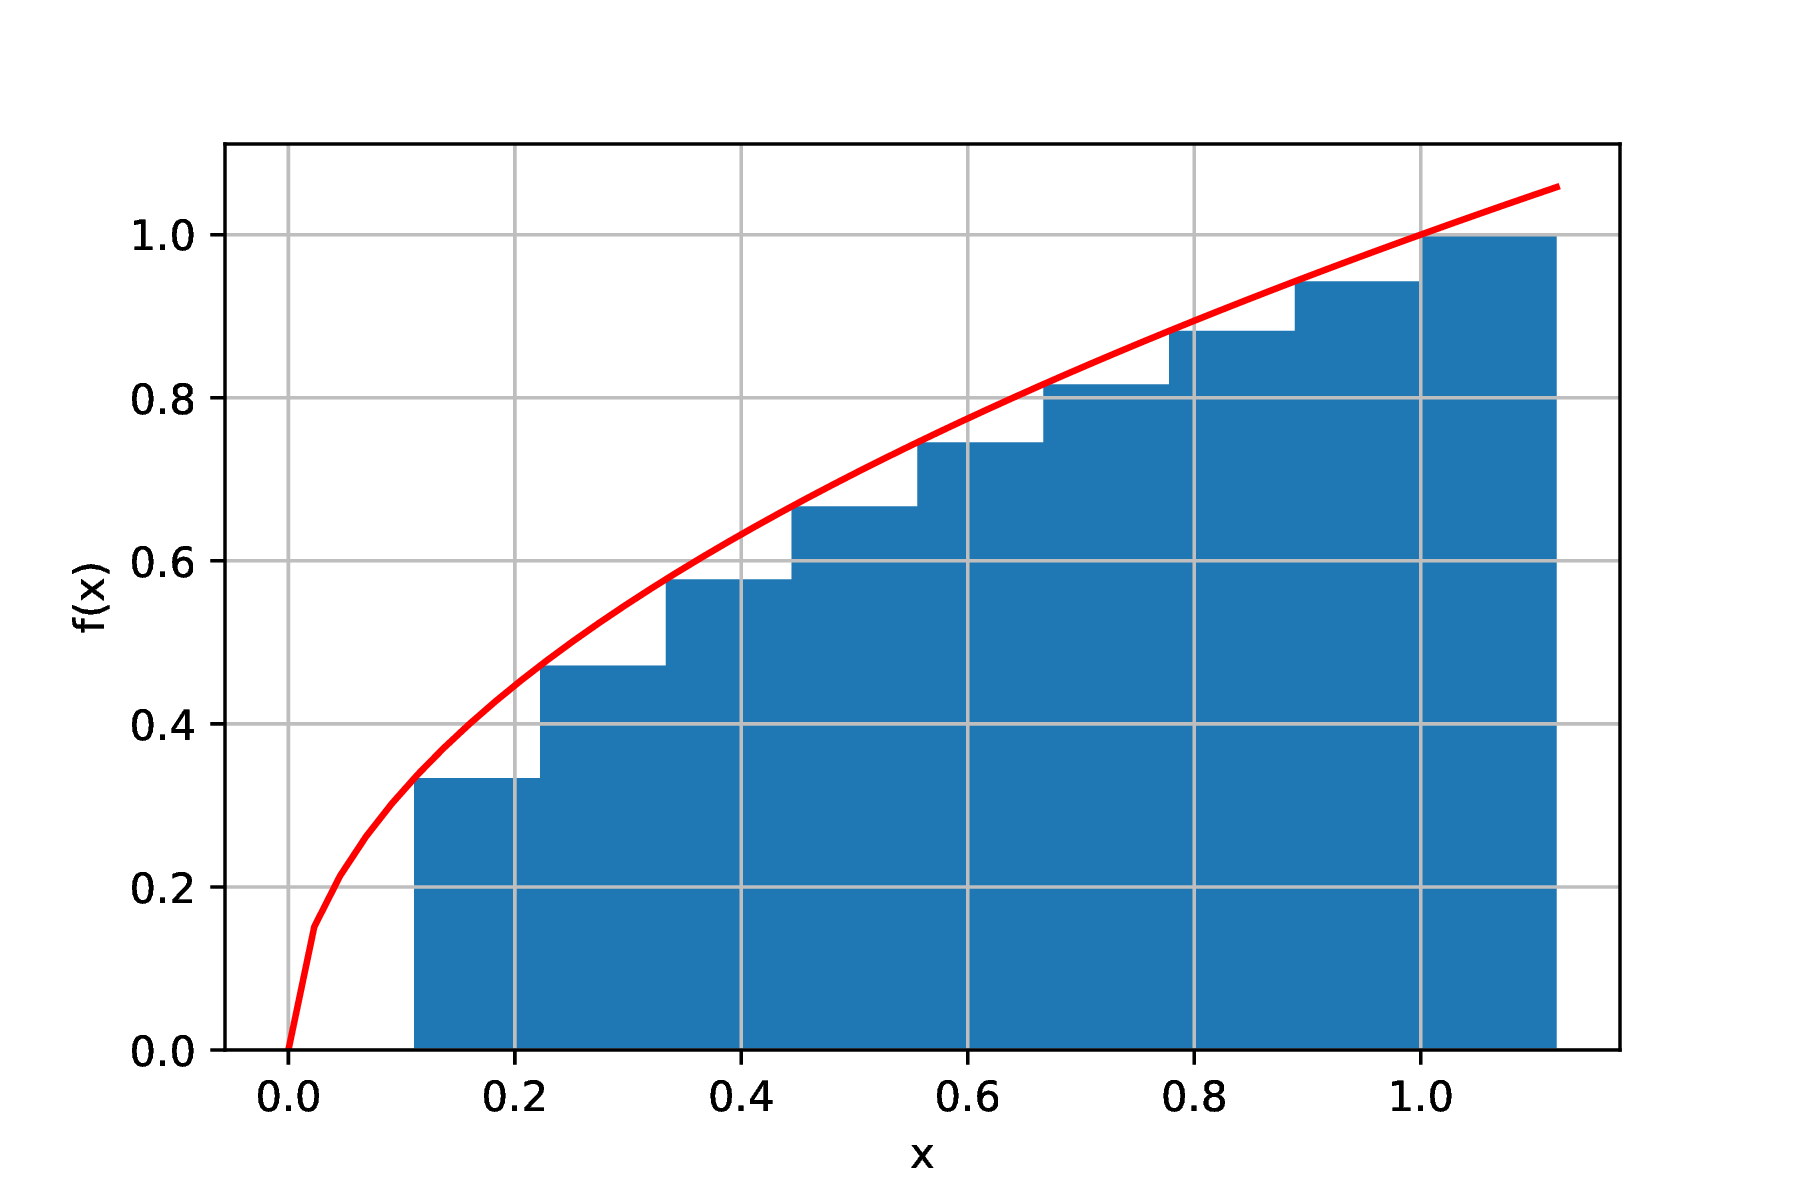
\includegraphics[width=1\linewidth]{plot.png}
    \end{figure}
    \column{0.5\linewidth}
    \begin{equation*}
       f(x) = \begin{cases}
        0 , &x < 0.12 \\
        0.35, &0.12 \leq x < 0.22\\
        0.47, &0.22 \leq x < 0.36\\
        \dots
        \end{cases}
    \end{equation*}
   \end{columns}
   
\end{frame}

%------------------------------------------------

\subsection{intuition}

\begin{frame}

\myframetitle{0.27\paperwidth}{0.04\paperwidth}{\insertsection}
\myframesubtitle{0.29\paperwidth}{\insertsubsection}

\vspace{0.25\paperheight}

\begin{textblock*}{.6\paperwidth}(0.05\paperwidth, 0.2\paperheight)
\begin{itemize}
	\item[\mybullet] What is the simplest way to categorize things?
	\item[\mybullet] Ask \textbf{yes/no questions}
\end{itemize}
\end{textblock*}

\vspace{0.05\paperheight}
\only<1>{
\begin{figure}
	\centering
	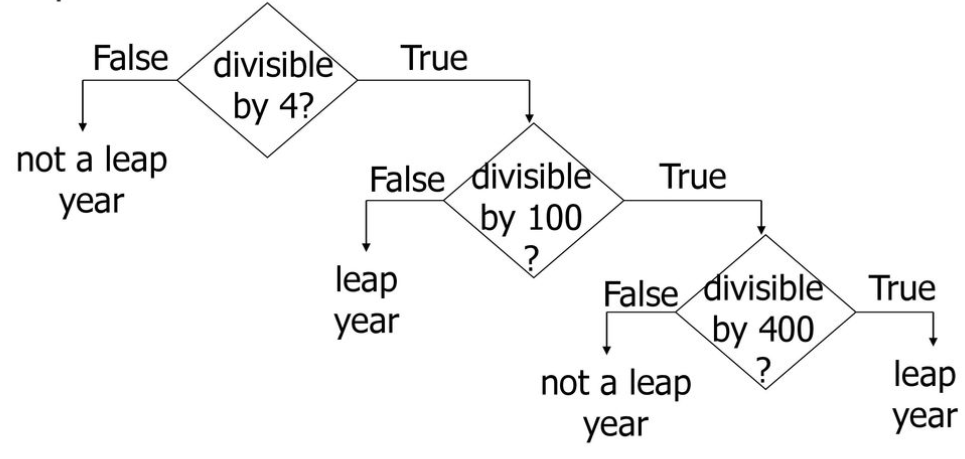
\includegraphics[width=0.6\textwidth]{leapyear.png}
\end{figure}
}

\only<2->{
\begin{figure}
	\centering
	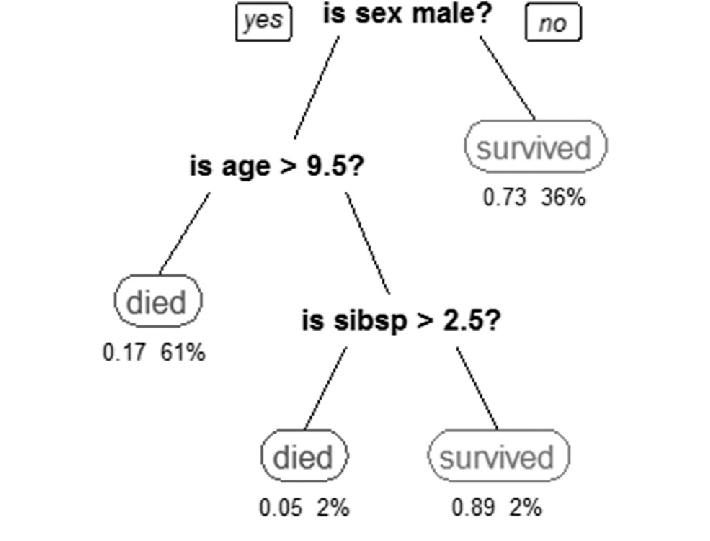
\includegraphics[width=0.35\textwidth]{titanic.png}
\end{figure}
}

\begin{textblock*}{.5\paperheight}(0.7\paperwidth, 0.6\paperheight)
	\only<3->{\textcolor{myorange}{Can we mathematically formulate this?}}
\end{textblock*}

%\vfill
%source: https://slideplayer.com/slide/12812756/
\end{frame}

%------------------------------------------------

\subsection{algorithm}
\begin{frame}
\myframetitle{0.27\paperwidth}{0.04\paperwidth}{\insertsection}
\myframesubtitle{0.29\paperwidth}{\insertsubsection}

\vspace{0.2\paperheight}
\begin{columns}
\column{0.55\linewidth}
\begin{algorithm}[H]
\begin{algorithmic}[1]
\small
\vspace{0.5ex}
\STATE Initialize: hyperparameters, leaf set = $\{\text{X}_\text{train}\}$
\vspace{0.5ex}
\WHILE{not stopping criteria}
\vspace{0.2ex}
\STATE leaf to split = Choose(leaf set)
\vspace{0.2ex}
\STATE left leaf, right leaf = Split(leaf to split)
\vspace{0.2ex}
\STATE Add left leaf, right leaf to leaf set
\STATE Remove leaf to split from leaf set
\vspace{0.2ex}
\ENDWHILE
\end{algorithmic}
\caption{Decision tree}
\label{alg:seq}
\end{algorithm}
\column{0.45\linewidth}
\centering
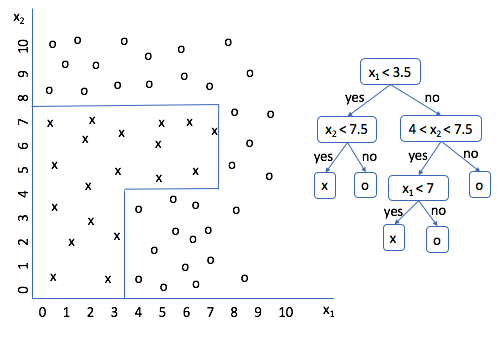
\includegraphics[width=1.\textwidth]{class_tree_scheme.png}
\end{columns}

\end{frame}

%------------------------------------------------

\subsection{split criteria}

\begin{frame}
\myframetitle{0.27\paperwidth}{0.04\paperwidth}{\insertsection}
\myframesubtitle{0.29\paperwidth}{\insertsubsection}

\vspace{0.2\paperheight}
\begin{columns}
	\begin{column}{0.6\textwidth}
		\begin{itemize}
%			\itemsep0.8ex
			\small
			\setbeamertemplate{items}{\mybullet}
			\item Suppose there is a classification problem
			\item So we want to separate one class from the other by constructing \textbf{decision boundary}
			\item And using decision tree algorithm described earlier
			\item To do that we need to start splitting on features
			\item Which \textbf{split} is the best?
			\item<2>[\textcolor{myorange}{\MVRightArrow}] \textcolor{myorange}{We need some criteria}
		\end{itemize}
	\end{column}
	
	\begin{column}{0.5\textwidth}
		\vspace{-0.05\paperheight}
		\begin{figure}
			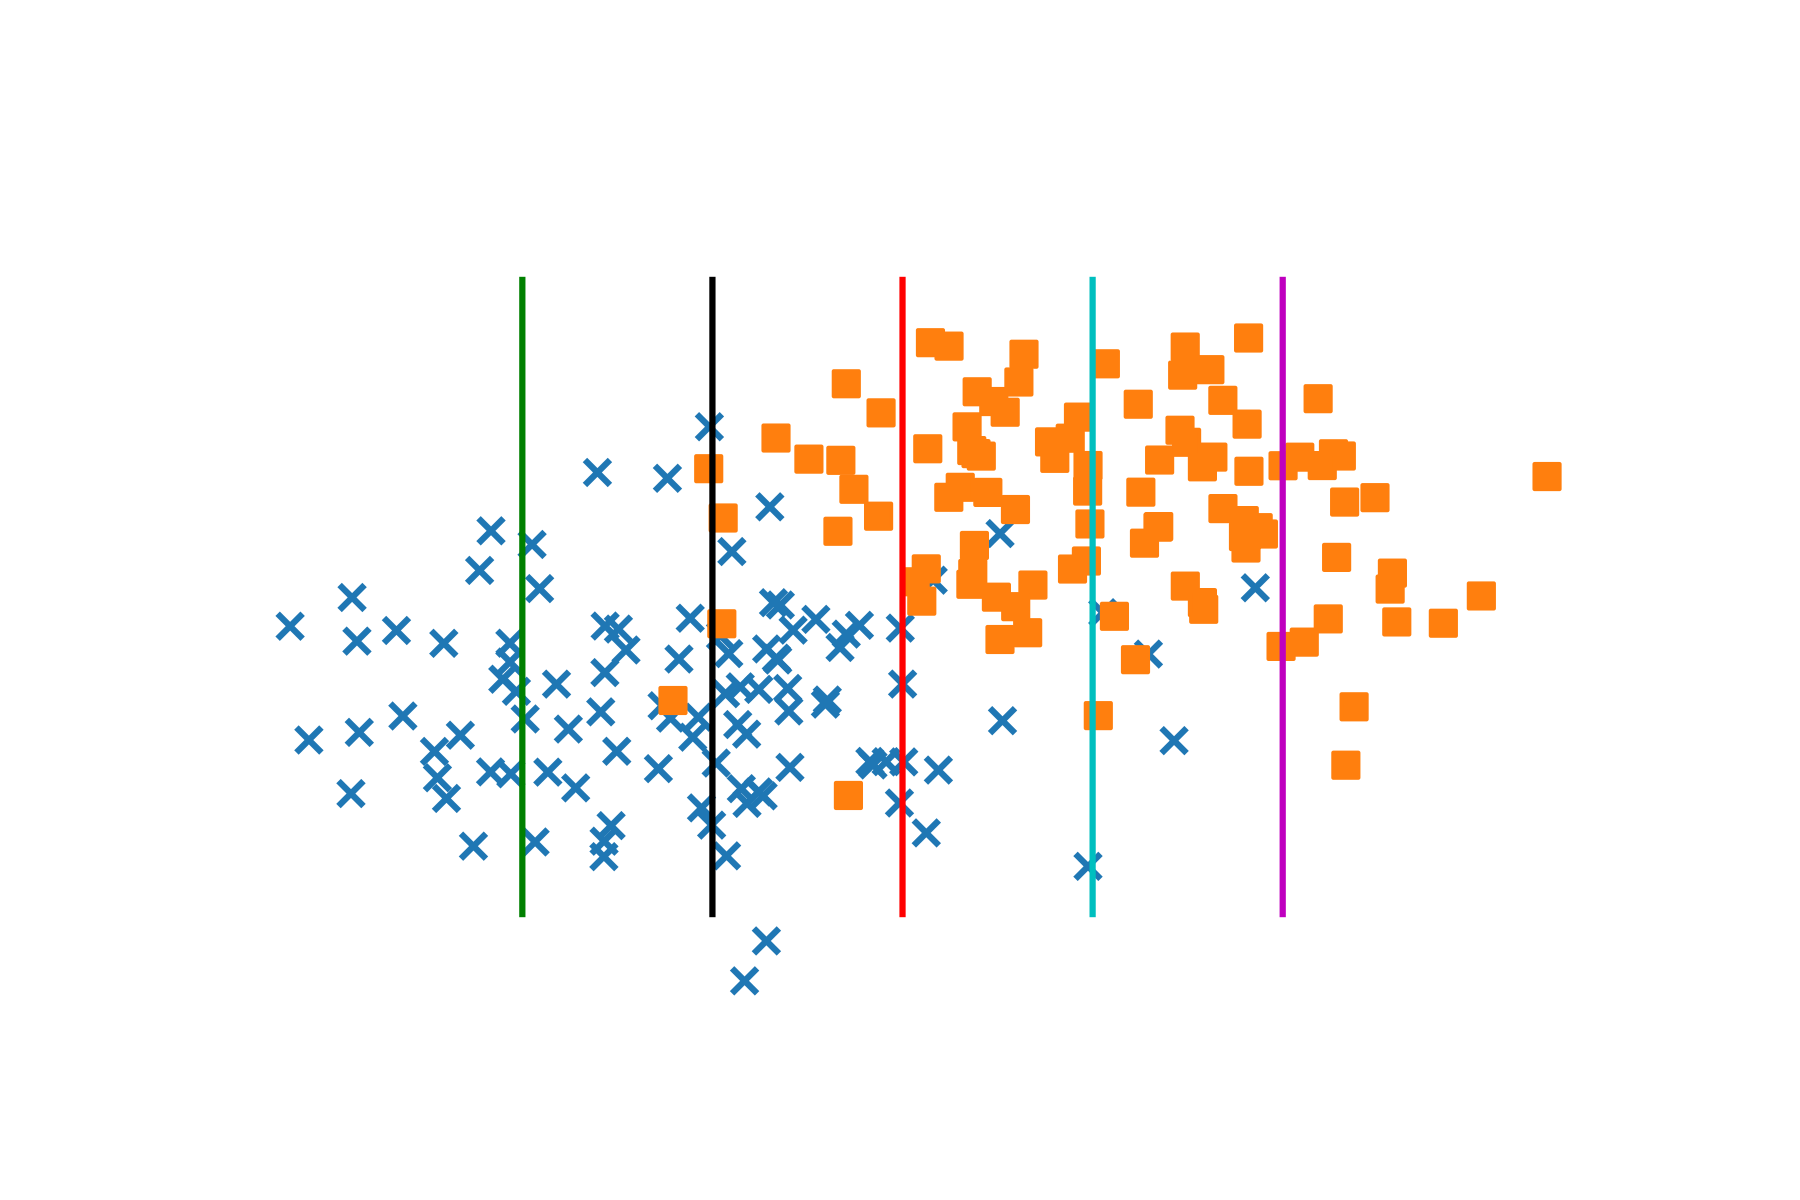
\includegraphics[width=1.\textwidth]{split.png}
		\end{figure}
	\end{column}
\end{columns}

\begin{textblock*}{.1\paperheight}(0.28\paperwidth, 0.71\paperheight)
	\only<2>{
\includegraphics[width=1.\textwidth]{Axe}}
\end{textblock*}

\end{frame}

%------------------------------------------------

\begin{frame}
\myframetitle{0.27\paperwidth}{0.04\paperwidth}{\insertsection}
\myframesubtitle{0.29\paperwidth}{\insertsubsection}

\vspace{0.1\paperheight}
\begin{columns}
\begin{column}{0.5\textwidth}
\begin{figure}
	\centering
	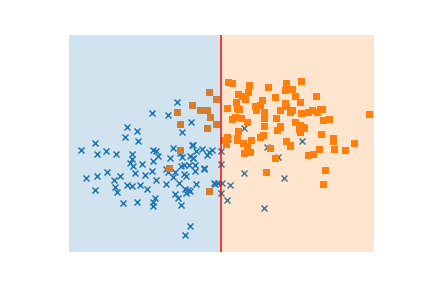
\includegraphics[width=1.\textwidth]{psplit.png}
\end{figure}
\end{column}

\begin{column}{0.5\textwidth}
\begin{figure}
	
\includegraphics[width=.3\textwidth]{Axe.png}
\end{figure}
\end{column}
\end{columns}

\vfill
The "best" split is a central one because it introduces \textbf{purity} in the best way. And we have some functions to measure the purity!
\end{frame}

%------------------------------------------------

\subsection{regression}
\begin{frame}
\myframetitle{0.27\paperwidth}{0.04\paperwidth}{\insertsection}
\myframesubtitle{0.29\paperwidth}{\insertsubsection}

\vspace{0.1\paperheight}
\begin{figure}
\centering
\only<1>{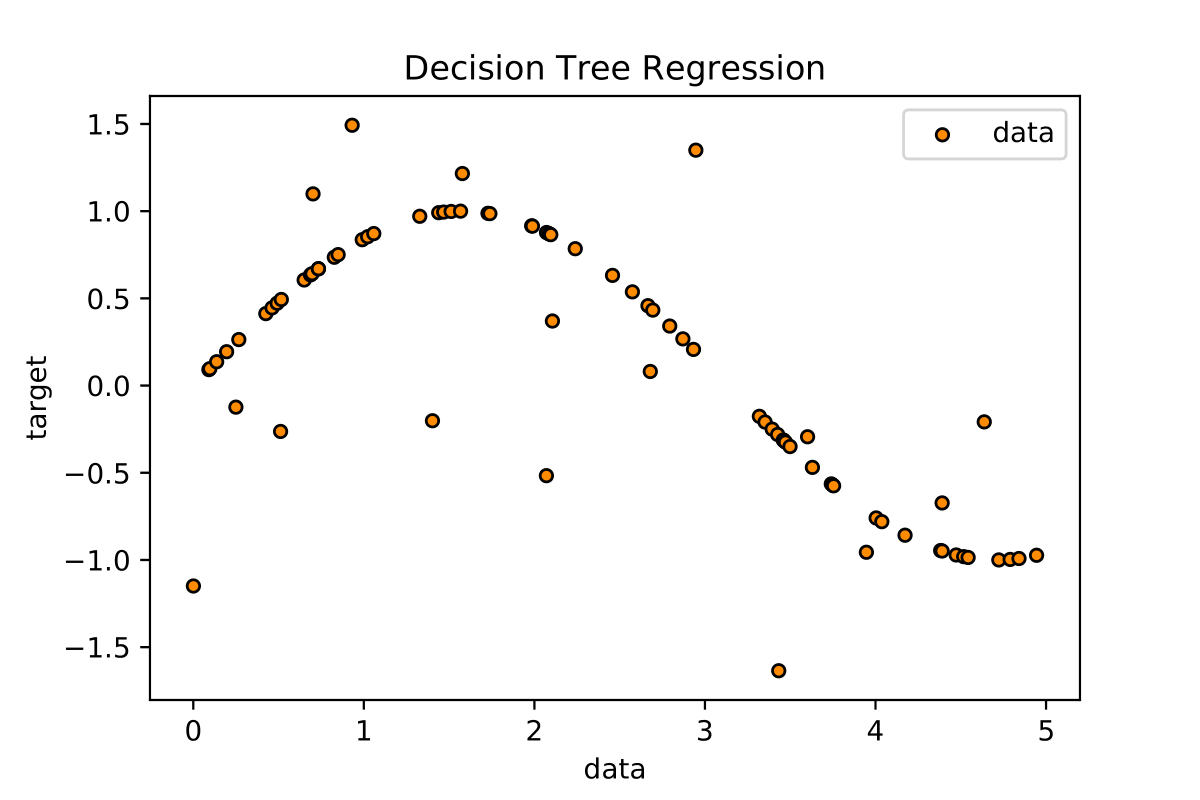
\includegraphics[width=0.6\textwidth]{regression.png}}
\only<2>{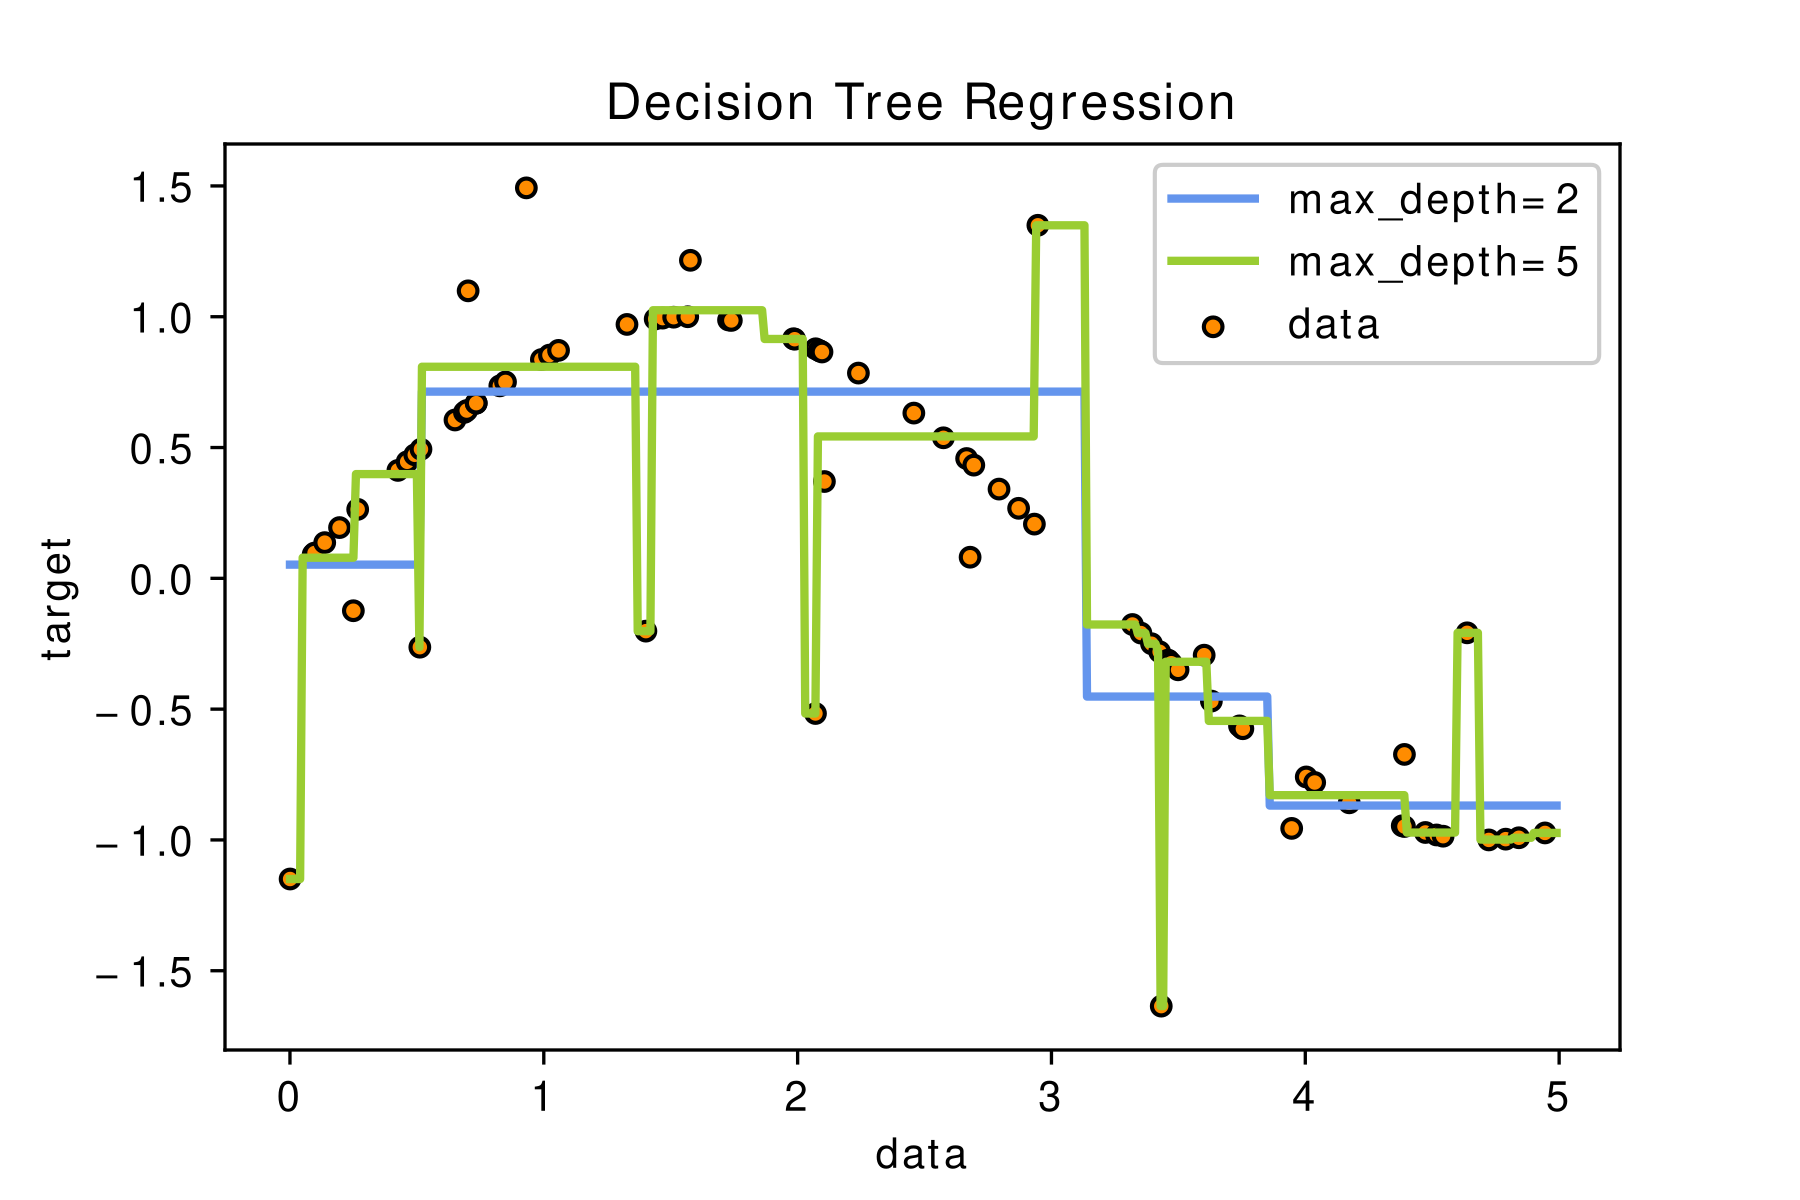
\includegraphics[width=0.6\textwidth]{dregr.png}}
\end{figure}
\centering
\small
Can we use decision tree approach for regression problem?
\only<2>{\textcolor{myorange}{Yes}}
\end{frame}

%------------------------------------------------

\subsection{growing}
\begin{frame}
\myframetitle{0.27\paperwidth}{0.04\paperwidth}{\insertsection}
\myframesubtitle{0.29\paperwidth}{\insertsubsection}

\vspace{-0.15\paperheight}
What about tree construction? \onslide<2->{\textcolor{myorange}{Do it recursively by \textbf{greedy} algorithm}}

\begin{textblock*}{1\paperwidth}(0.02\paperwidth, 0.35\paperheight)
	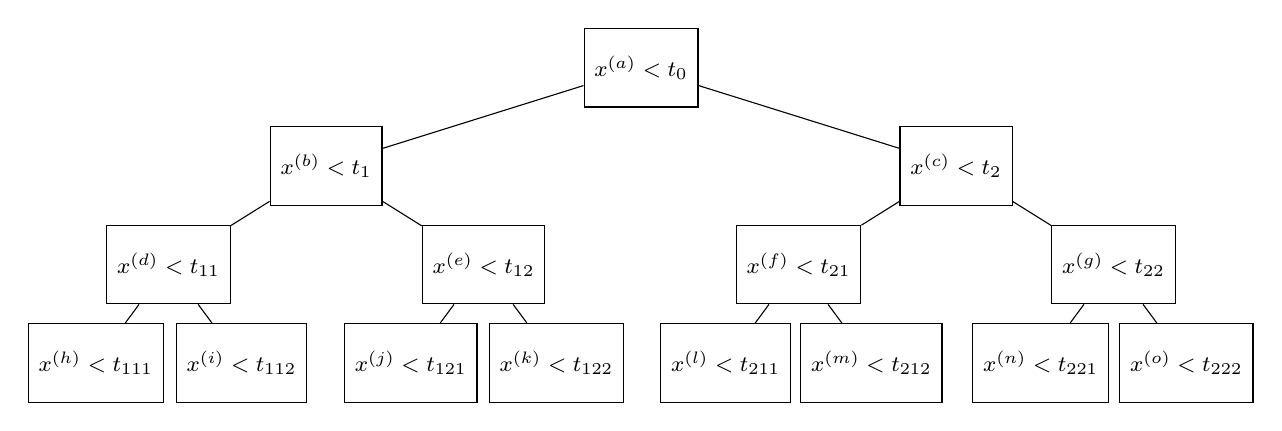
\begin{tikzpicture}[scale=0.5]
	\footnotesize	
	\node [arn_n] {$x^{(a)} < t_0$}
	child[visible on=<2->]{ node [arn_n] {$x^{(b)} < t_1$}
		child[visible on=<3->]{ node [arn_n] {$x^{(d)} < t_{11}$}
			child[visible on=<4->]{ node [arn_n] {$x^{(h)} < t_{111}$}}
			child[visible on=<4->]{ node [arn_n] {$x^{(i)} < t_{112}$}}                          
		}
		child[visible on=<3->]{ node [arn_n] {$x^{(e)} < t_{12}$}  
			child[visible on=<4->]{ node [arn_n] {$x^{(j)} < t_{121}$}}
			child[visible on=<4->]{ node [arn_n] {$x^{(k)} < t_{122}$}}                          
		}
	}
	child[visible on=<2->]{ node [arn_n] {$x^{(c)} < t_2$}
		child[visible on=<3->]{ node [arn_n] {$x^{(f)} < t_{21}$}
			child[visible on=<4->]{ node [arn_n] {$x^{(l)} < t_{211}$}}
			child[visible on=<4->]{ node [arn_n] {$x^{(m)} < t_{212}$}}                          
		}
		child[visible on=<3->]{ node [arn_n] {$x^{(g)} < t_{22}$}  
			child[visible on=<4->]{ node [arn_n] {$x^{(n)} < t_{221}$}}
			child[visible on=<4->]{ node [arn_n] {$x^{(o)} < t_{222}$}}                          
		}
	}
	%	}
	%}
	; 
	\end{tikzpicture} 
\end{textblock*}

\end{frame}

%------------------------------------------------

%\subsection{examples}
\begin{frame}
\myframetitle{0.27\paperwidth}{0.04\paperwidth}{\insertsection}
\myframesubtitle{0.29\paperwidth}{\insertsubsection}

\vspace{0.05\paperheight}
\begin{columns}
\begin{column}{0.5\textwidth}
	
	\only<1>{
		\begin{figure}
			\centering
			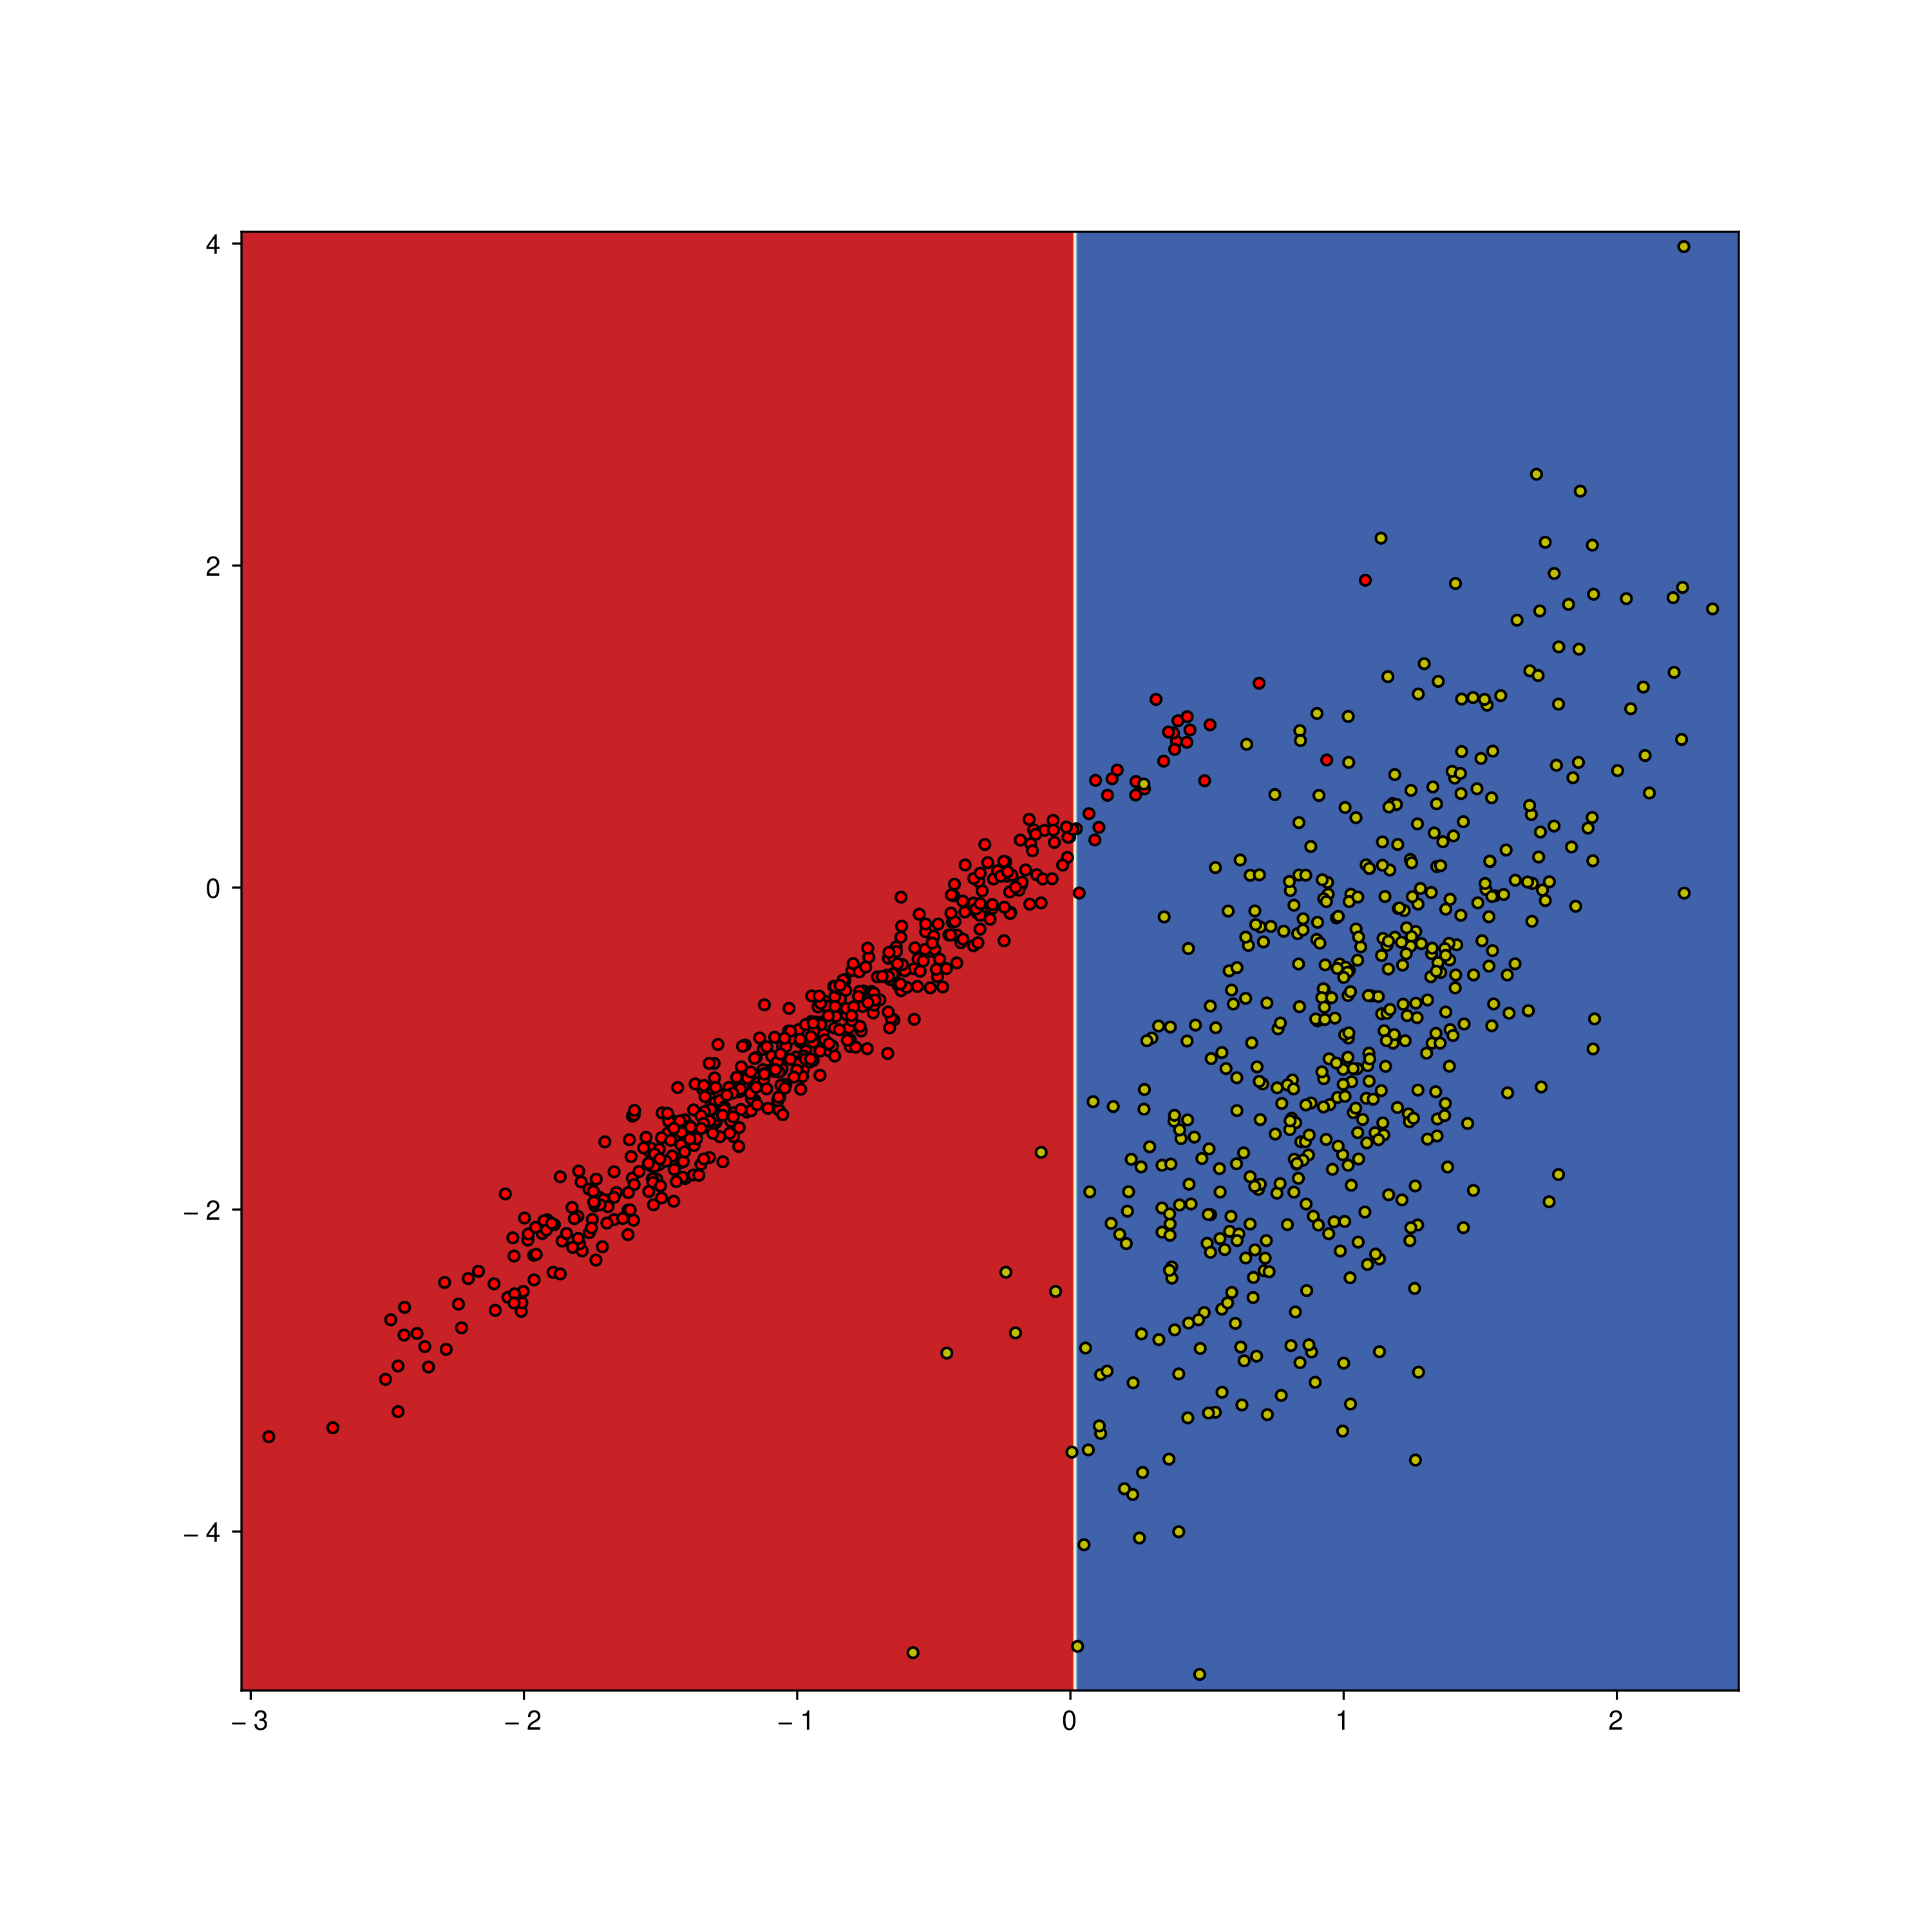
\includegraphics[width=0.7\textheight]{1gi.png}
		\end{figure}
	}
	
	\only<2>{
		\begin{figure}
			\centering
			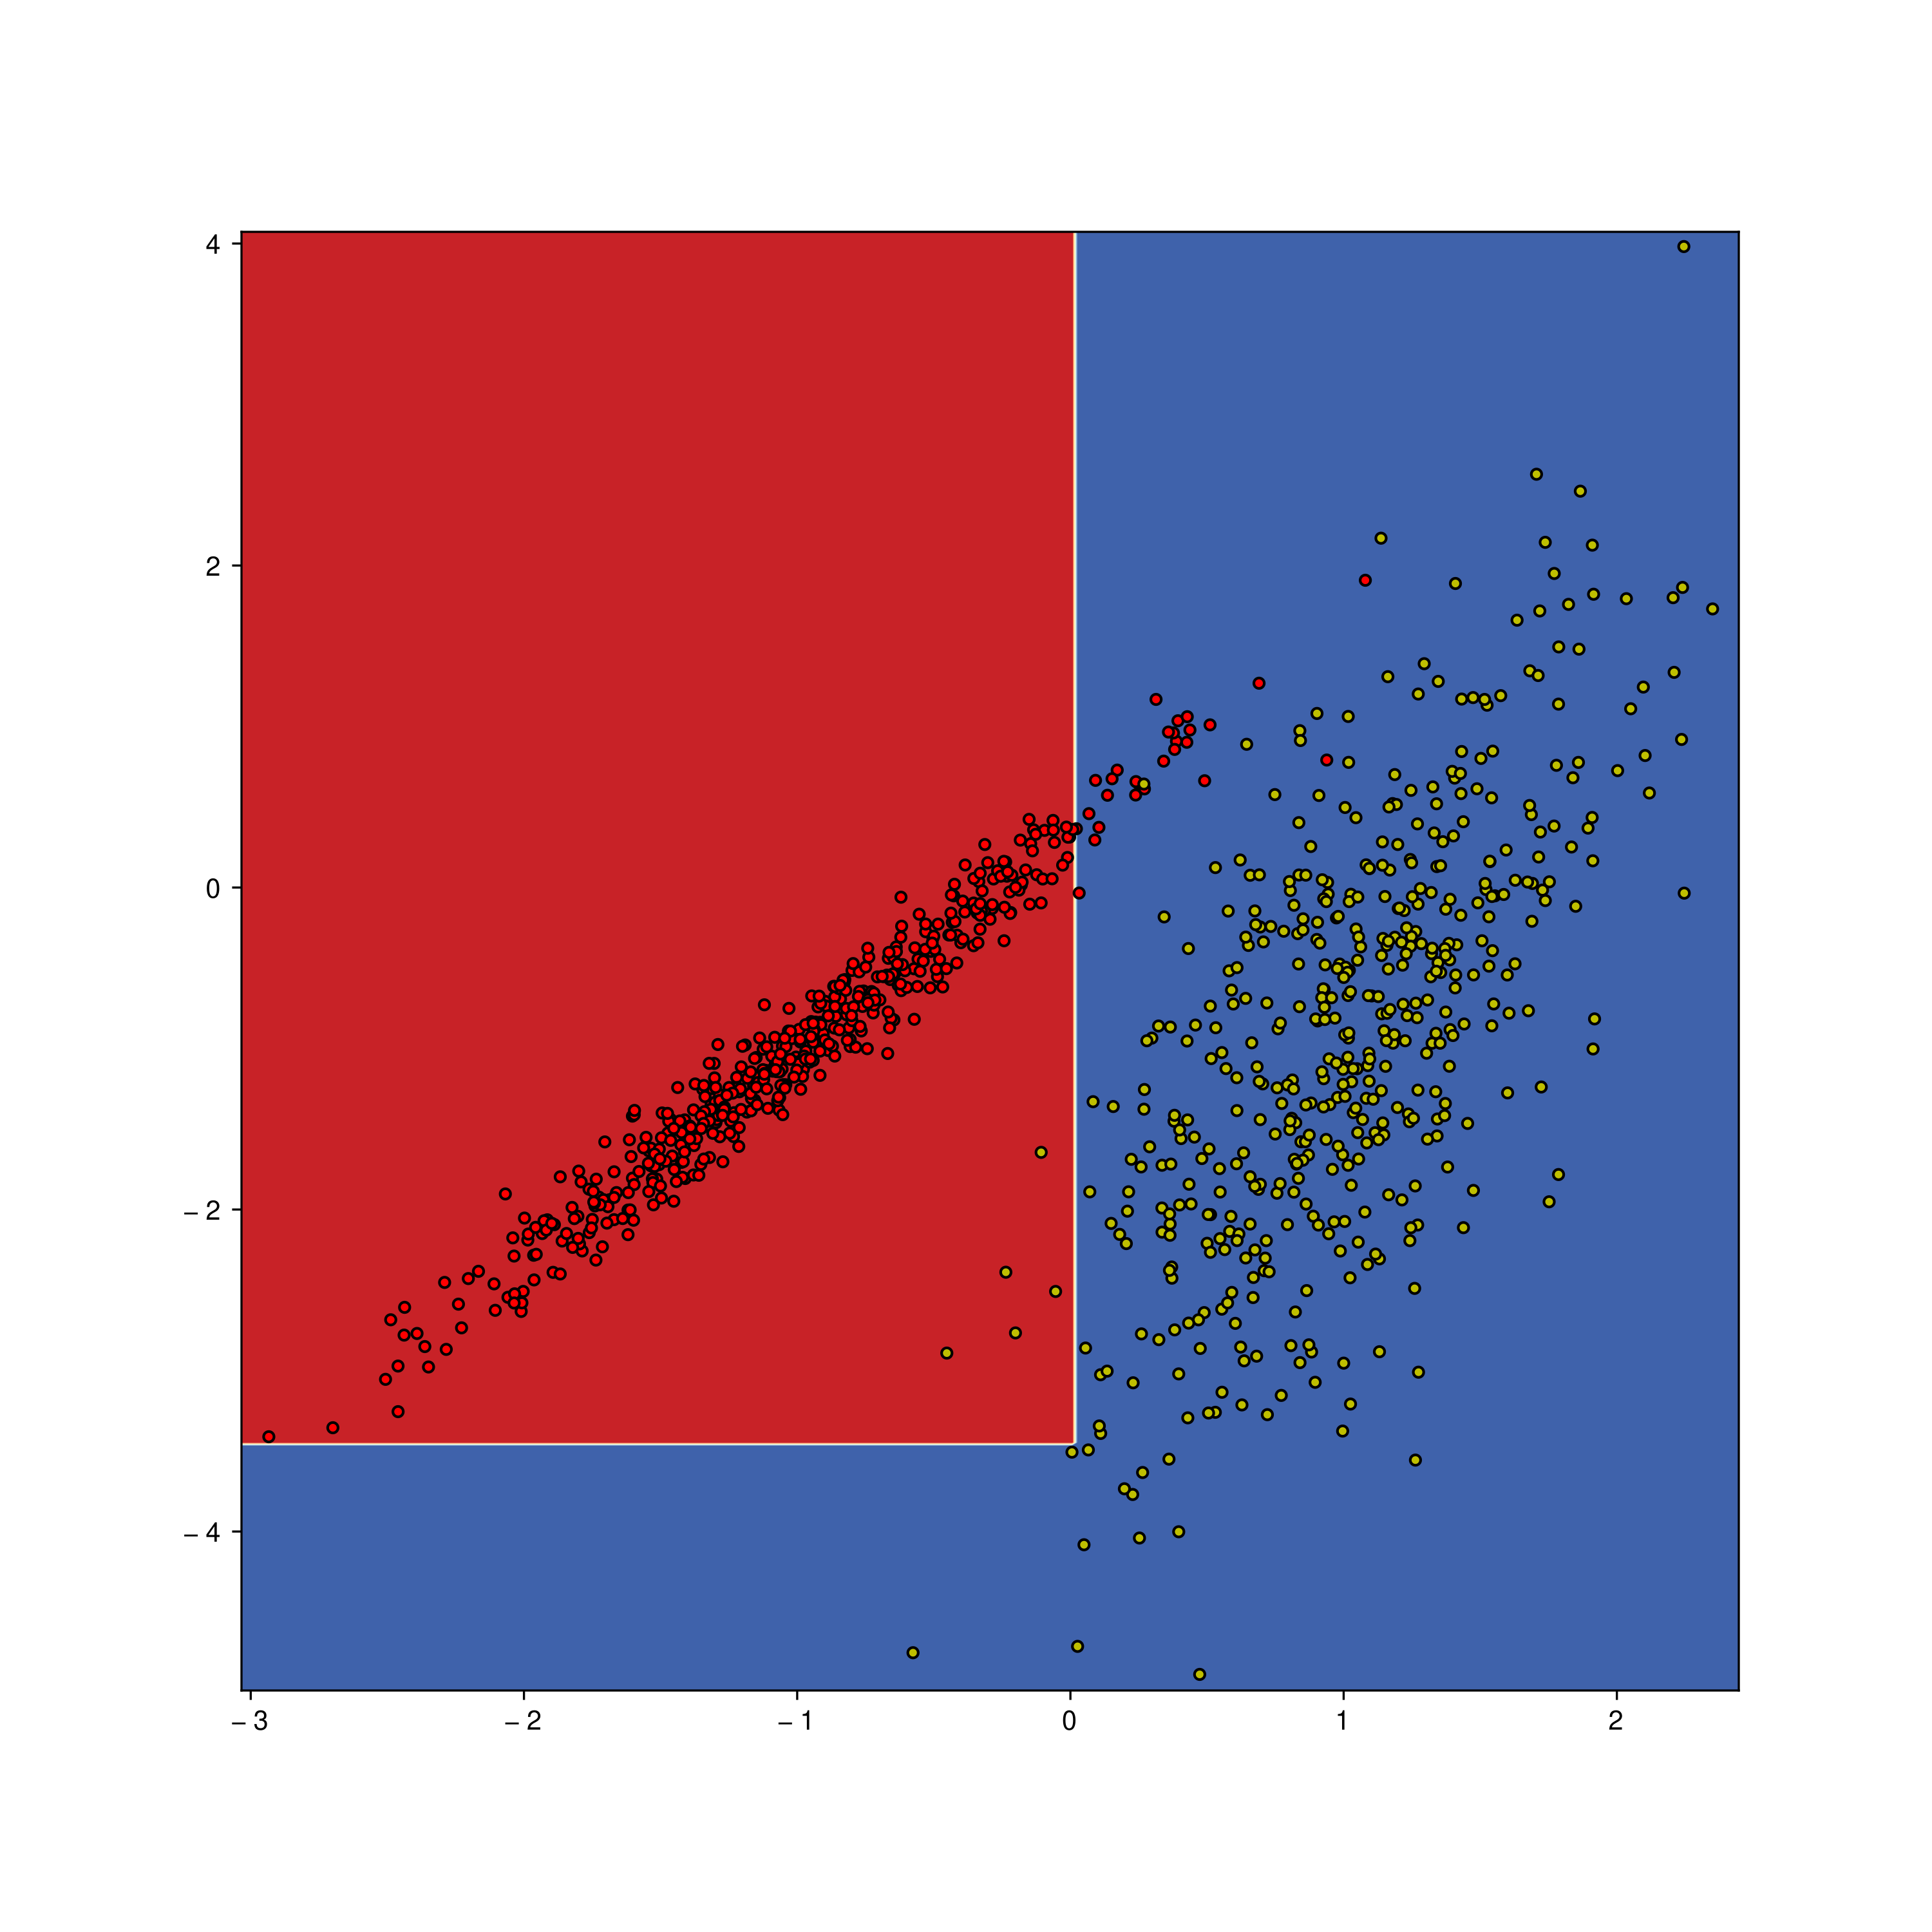
\includegraphics[width=0.7\textheight]{2gi.png}
		\end{figure}
	}
	
	\only<3>{
		\begin{figure}
			\centering
			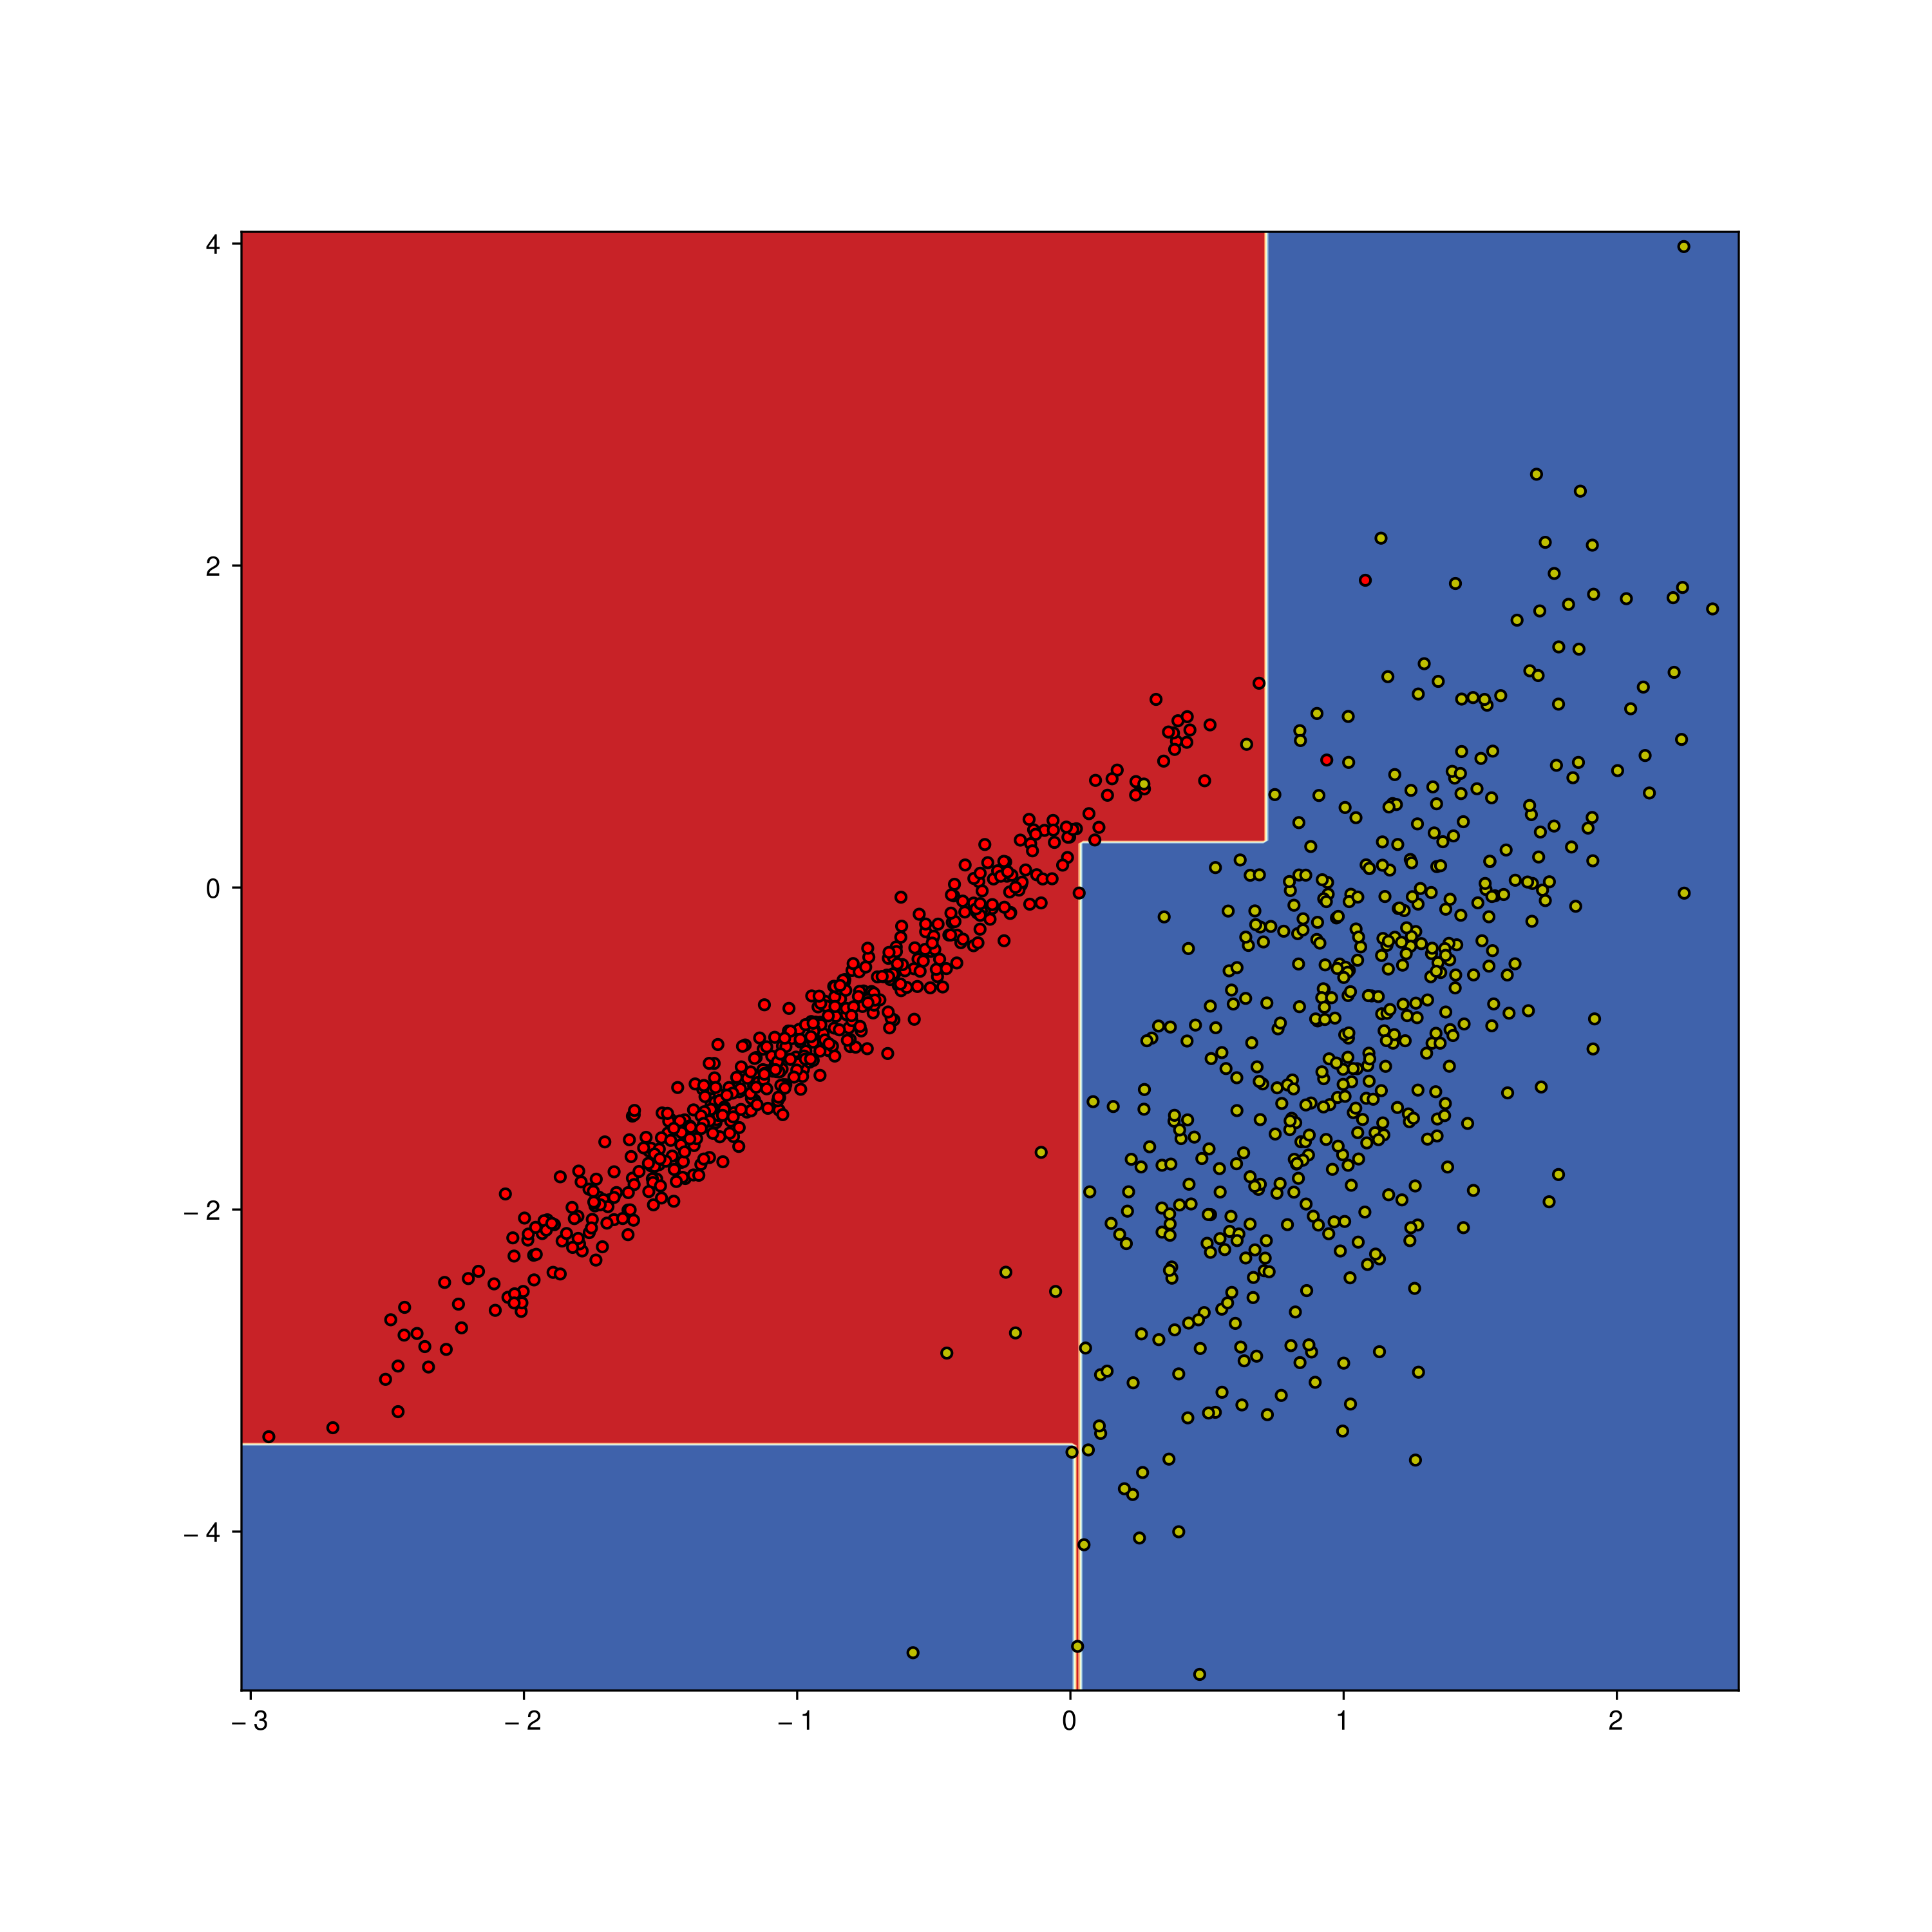
\includegraphics[width=0.7\textheight]{3gi.png}
		\end{figure}
	}
	
	\only<4>{
		\begin{figure}
			\centering
			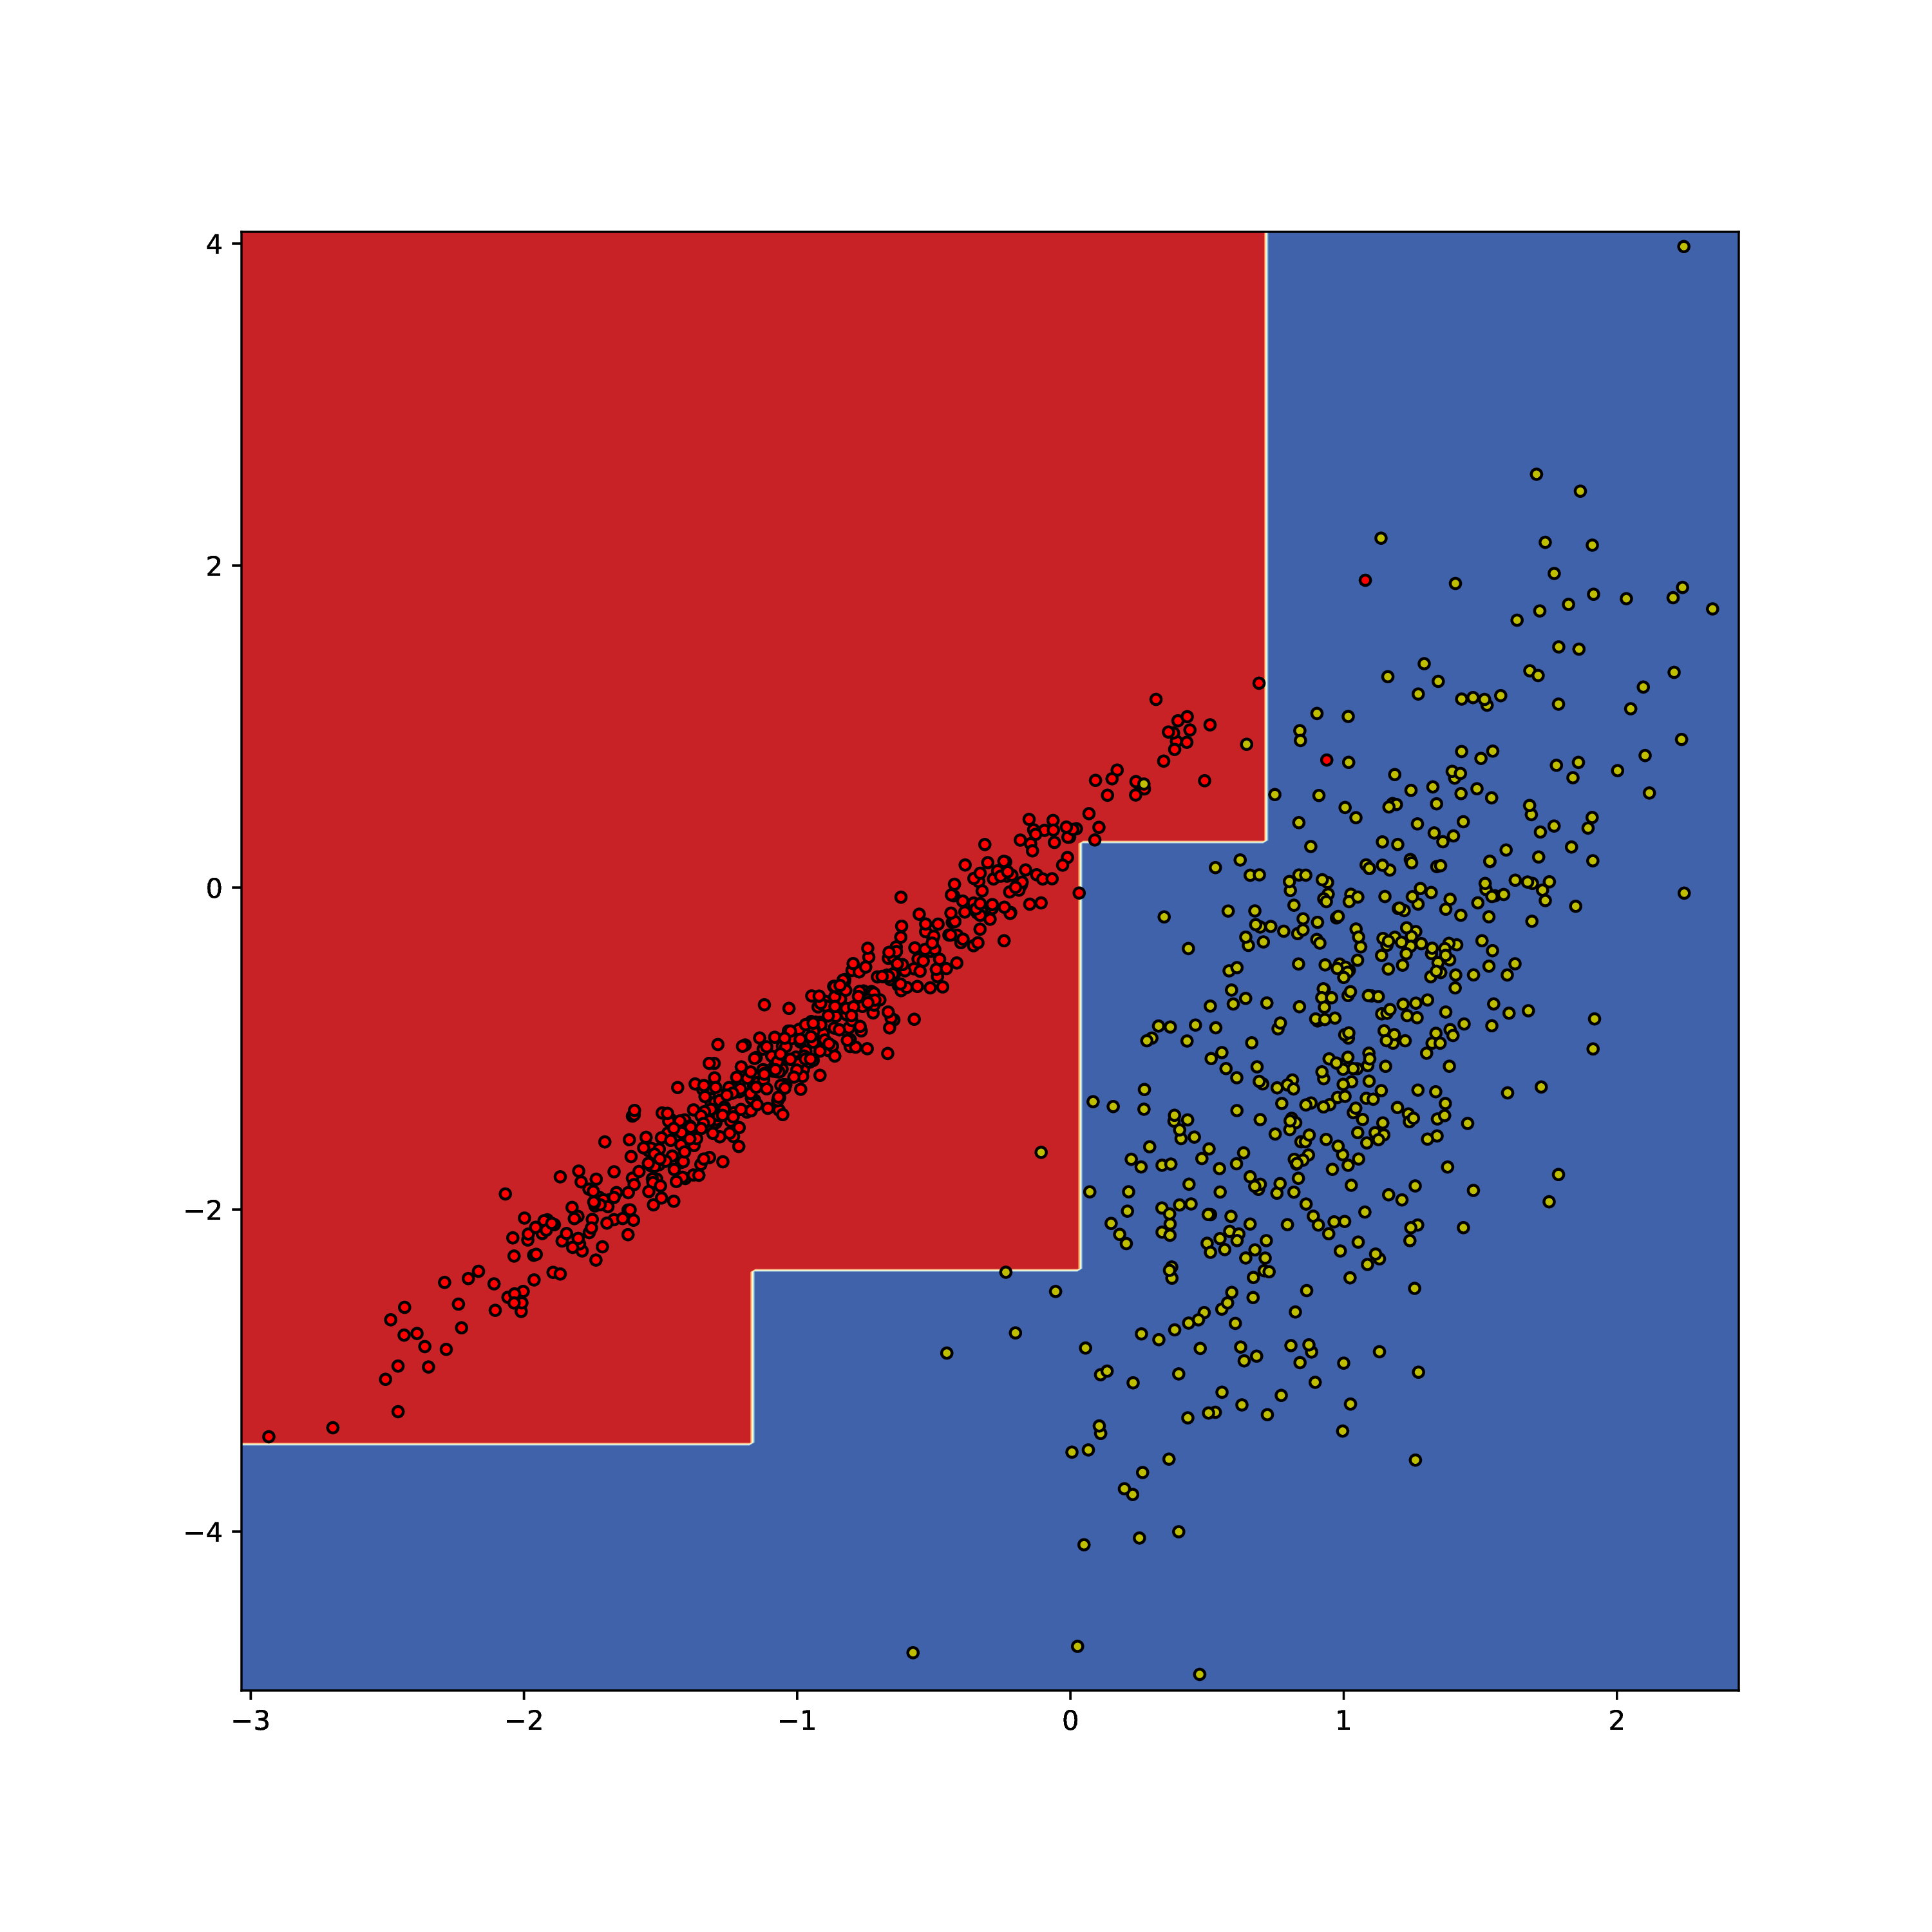
\includegraphics[width=0.7\textheight]{4gi.png}
		\end{figure}
	}
\end{column}

\begin{column}{0.5\textwidth}
	
	\only<1>{
	\begin{figure}
		\centering
		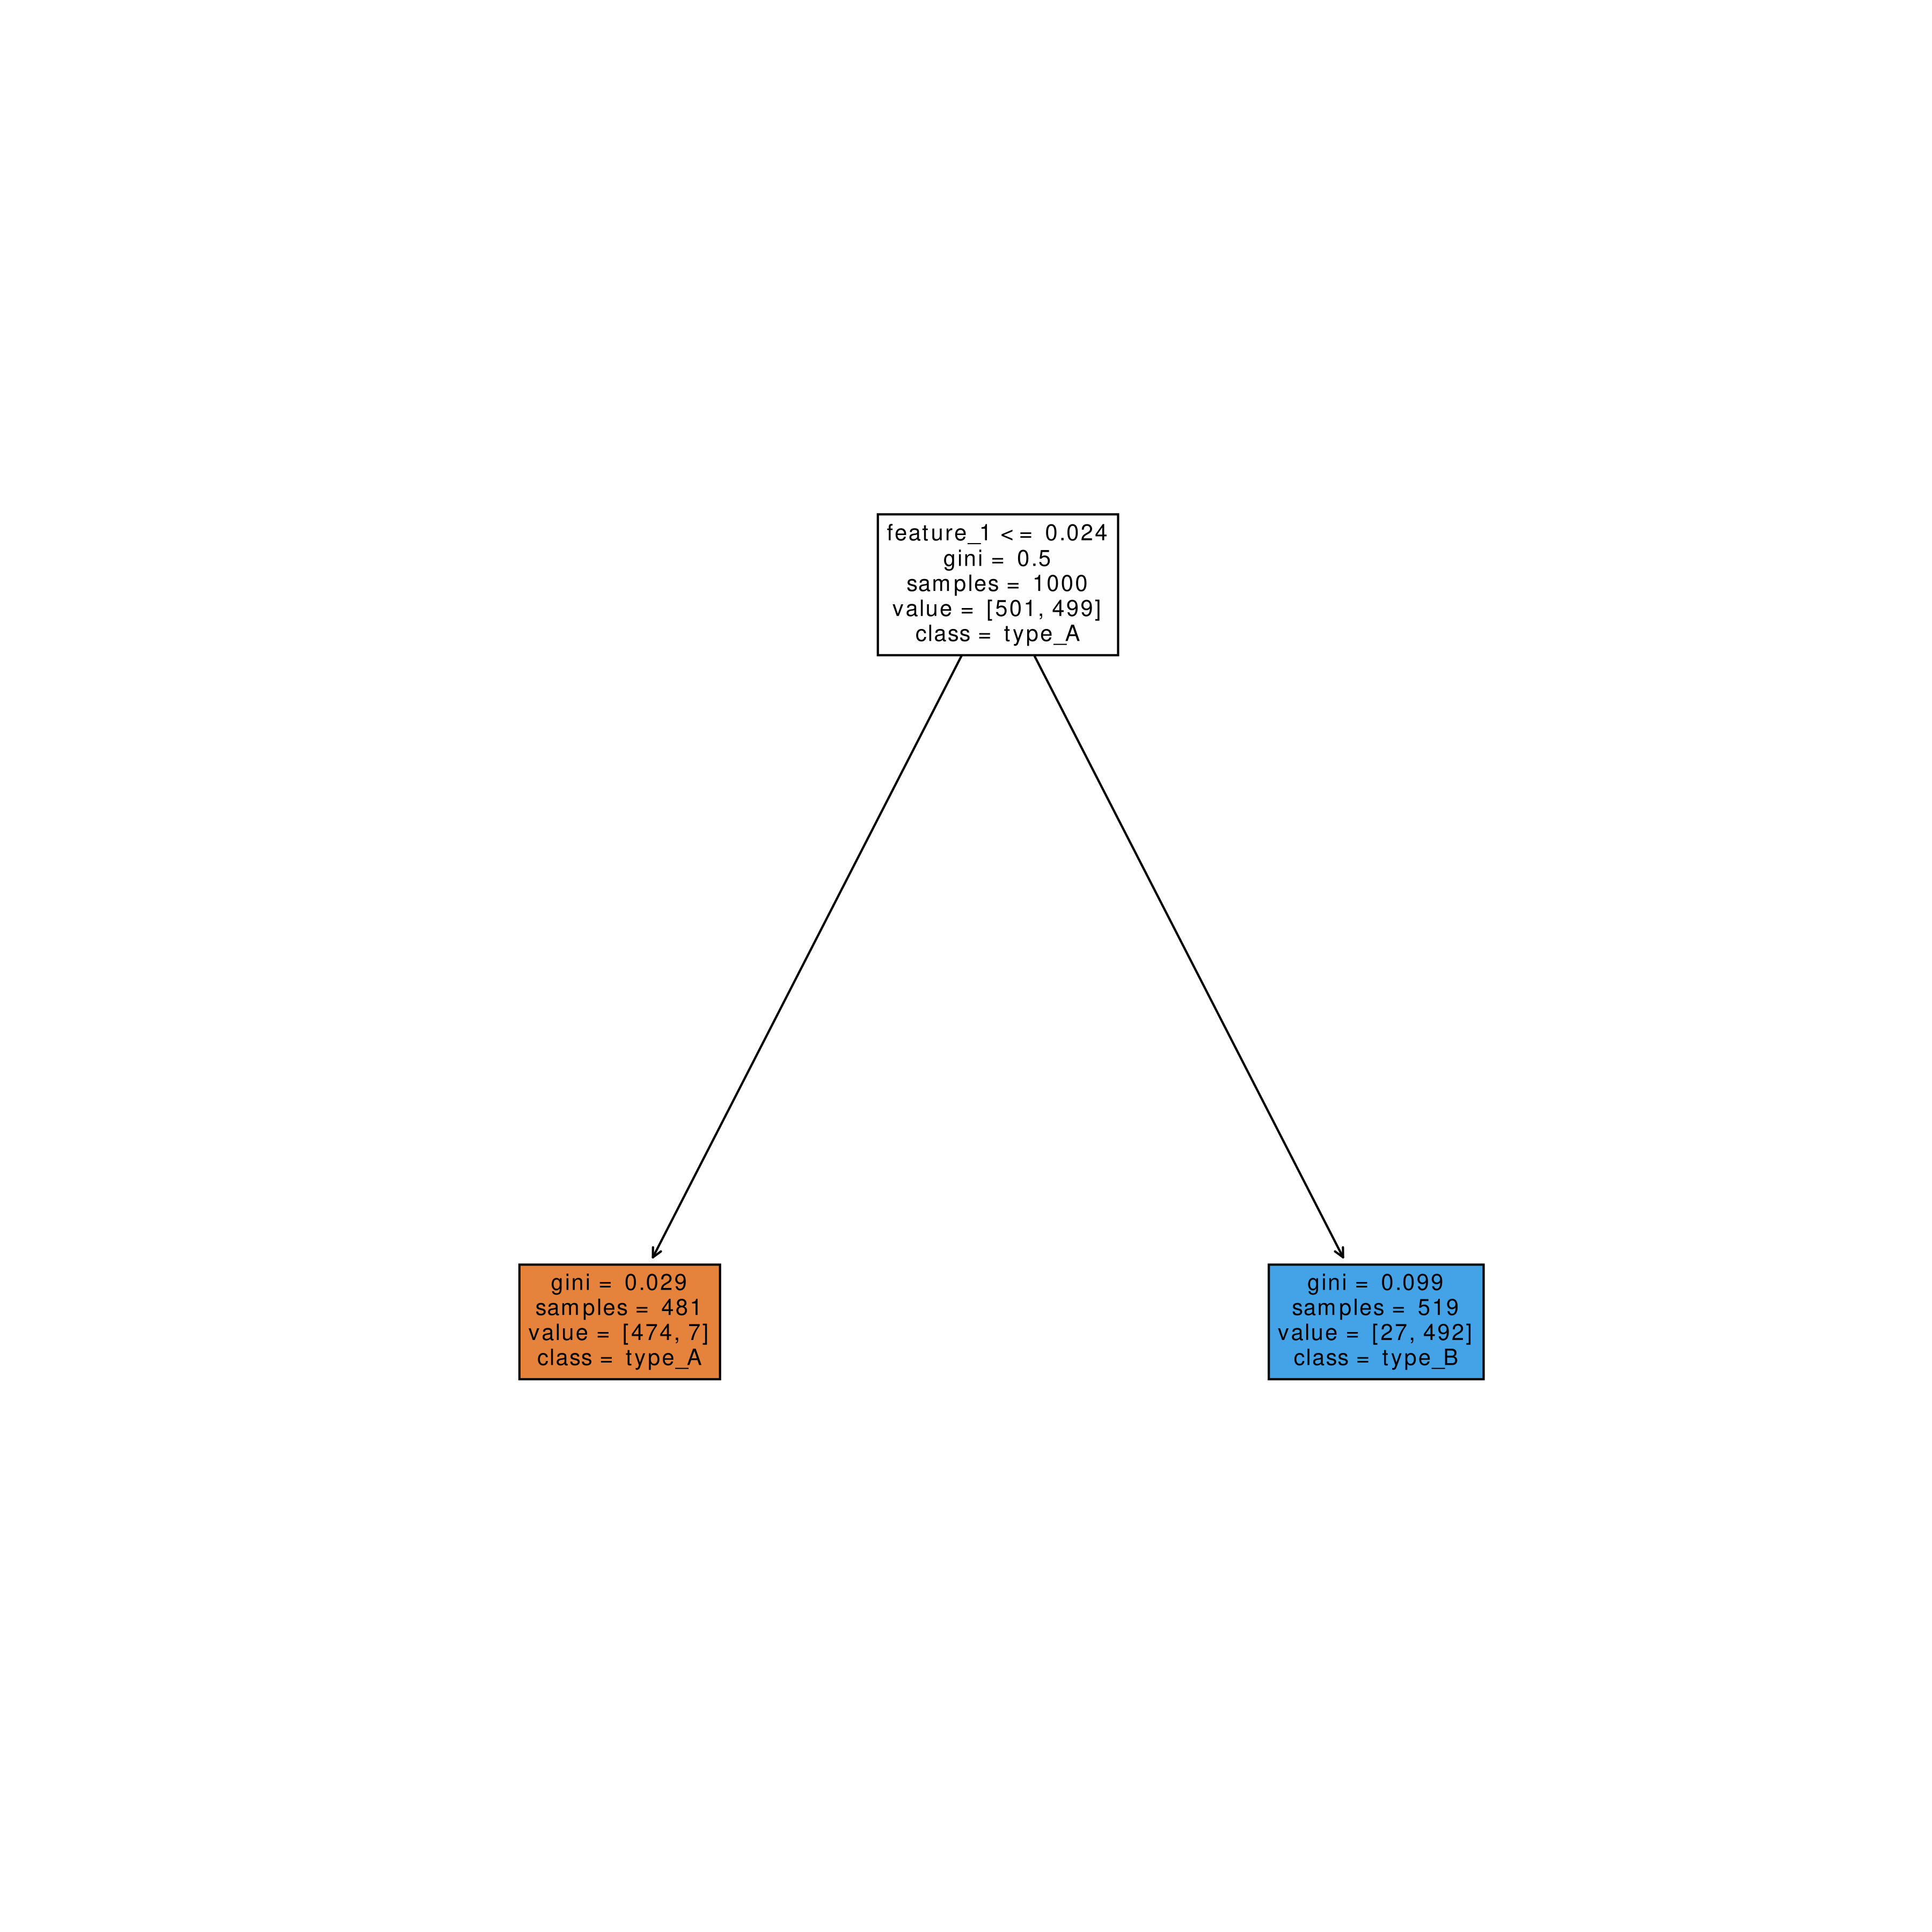
\includegraphics[width=0.9\textheight]{1tree.png}
	\end{figure}
}

	\only<2>{
	\begin{figure}
		\centering
		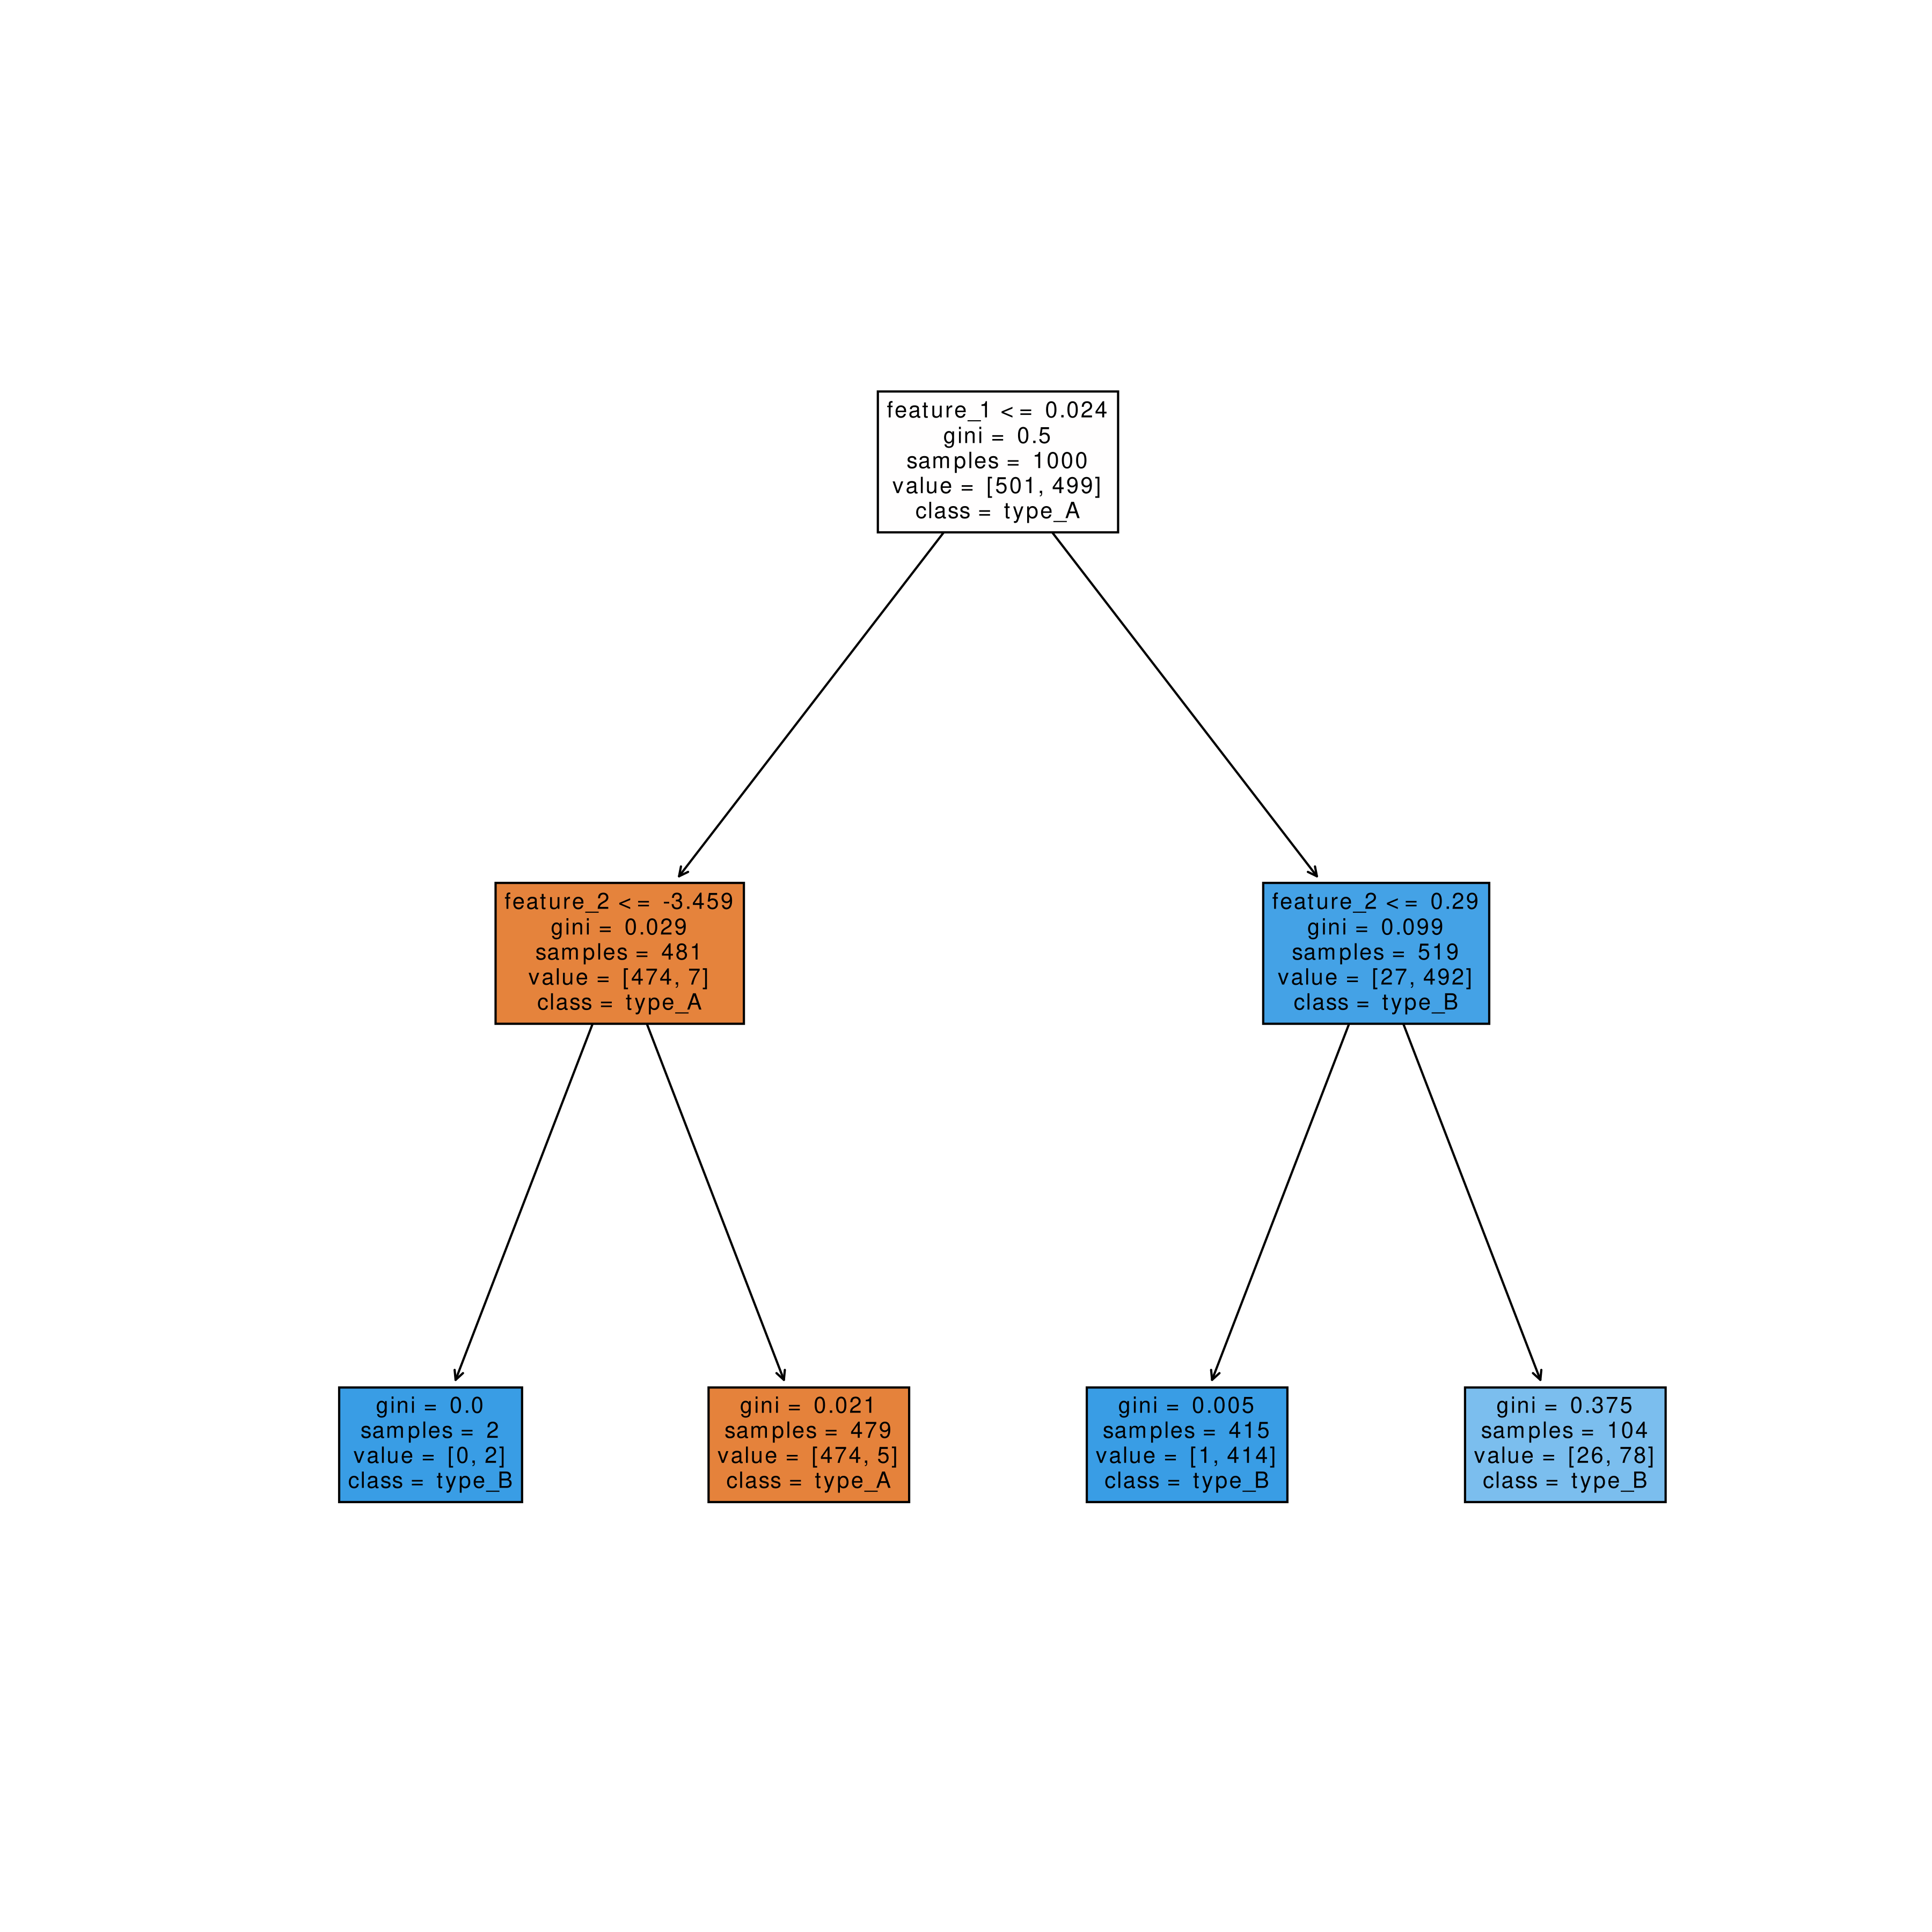
\includegraphics[width=0.9\textheight]{2tree.png}
	\end{figure}
}

	\only<3>{
	\begin{figure}
		\centering
		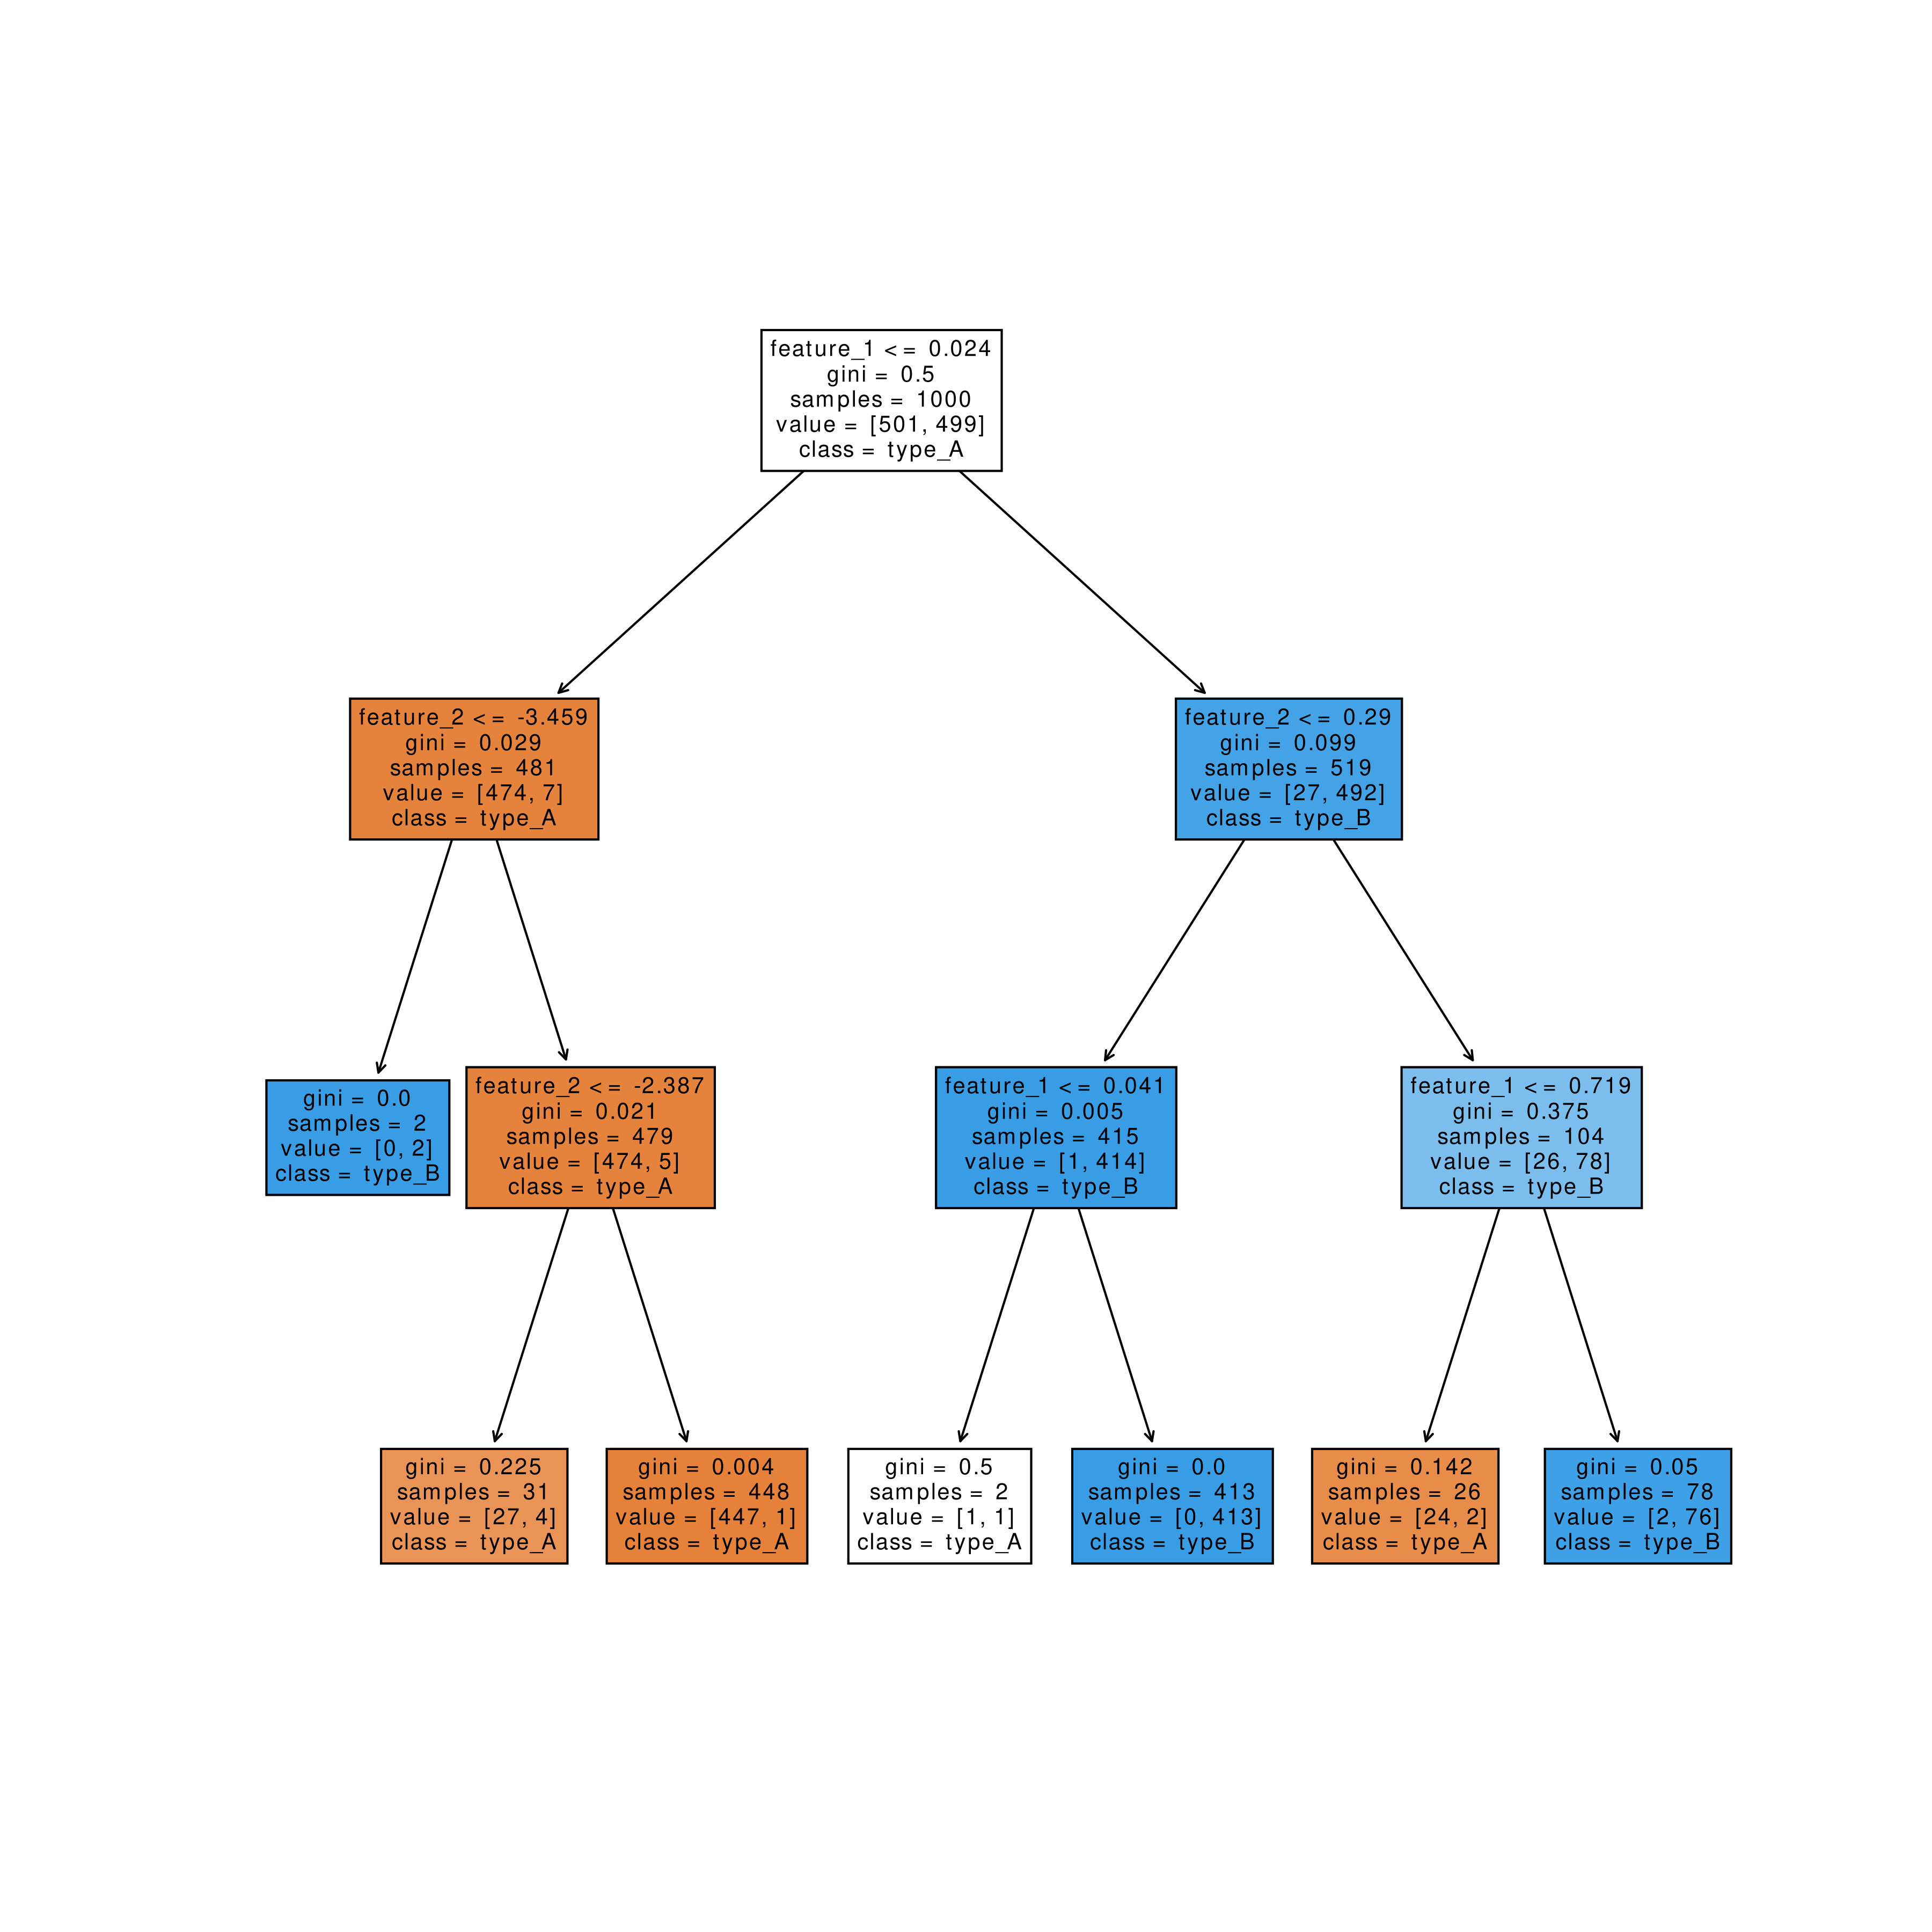
\includegraphics[width=0.9\textheight]{3tree.png}
	\end{figure}
}

	\only<4>{
	\begin{figure}
		\centering
		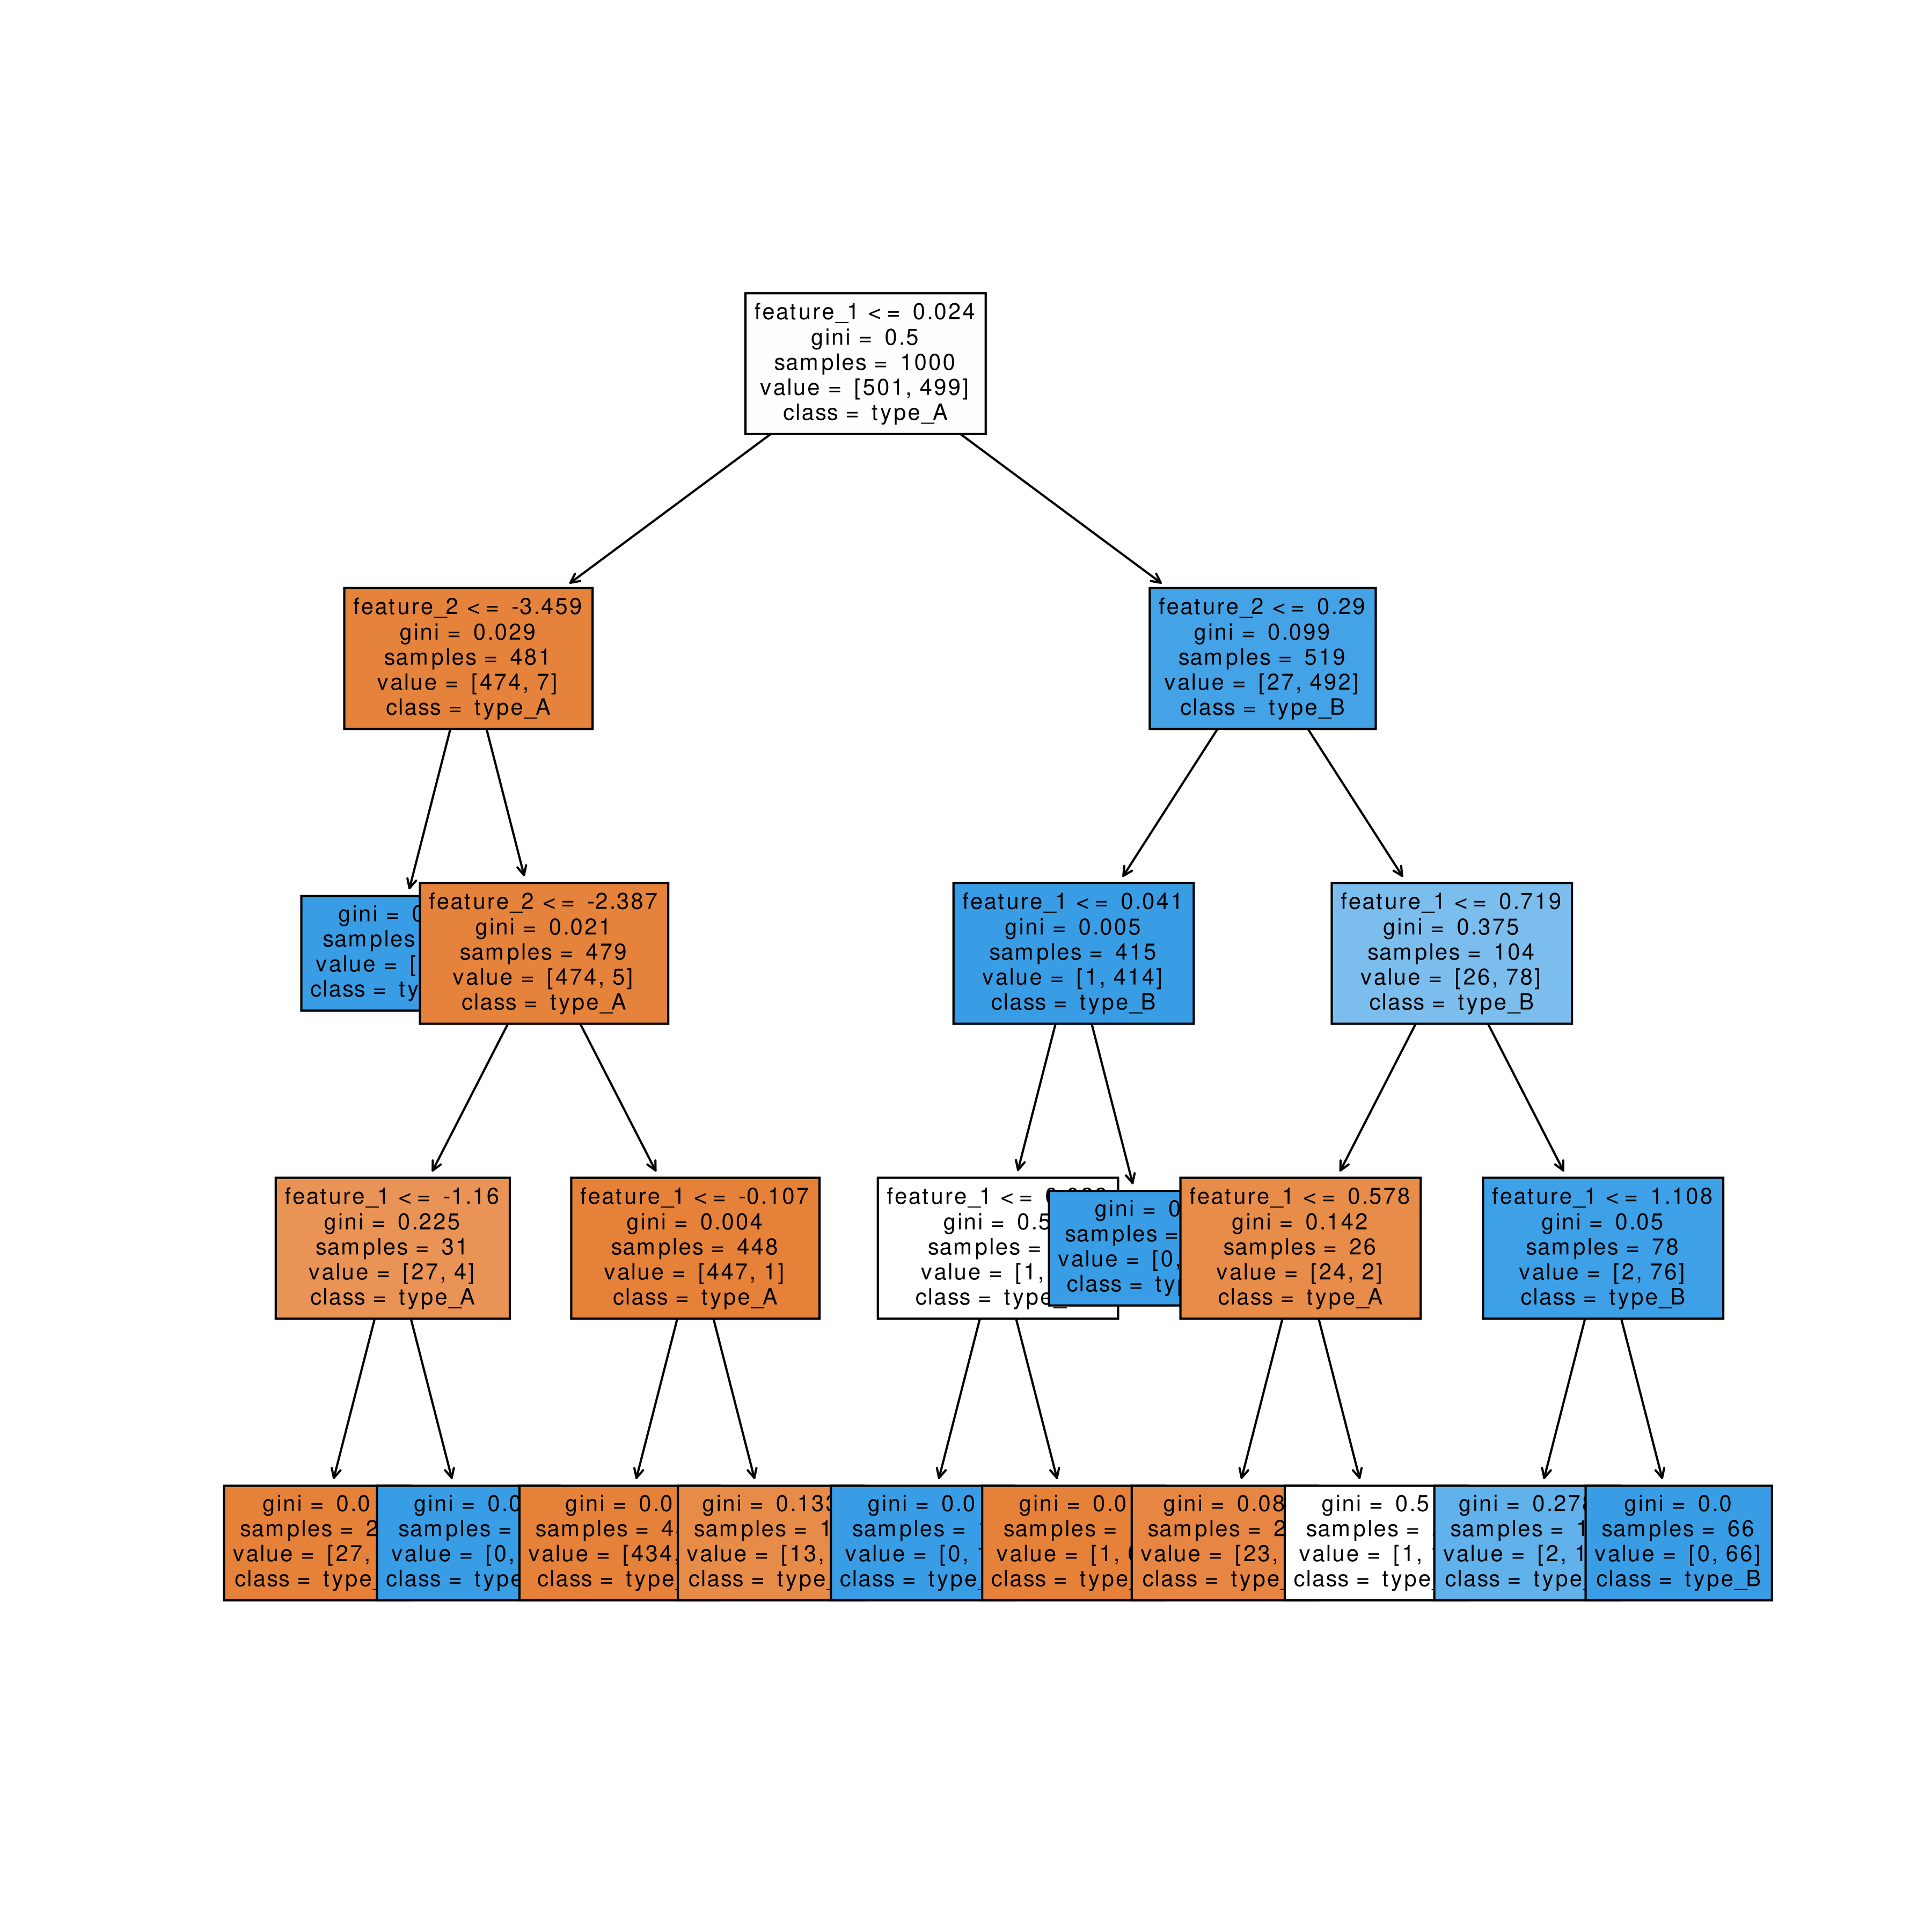
\includegraphics[width=0.9\textheight]{4tree.png}
	\end{figure}
}
\end{column}
\end{columns}


\begin{textblock*}{0.45\paperwidth}(0.7\paperwidth,0.1\paperheight)
	\footnotesize
	\textcolor{Gray}{check out also \href{http://www.r2d3.us/visual-intro-to-machine-learning-part-1/}{\underline{these}} visuals}
\end{textblock*}


\end{frame}

%------------------------------------------------
%------------------------------------------------
\section{Random forest and gradient boosting}
%------------------------------------------------
%------------------------------------------------

\begin{frame}[plain]
\centering
\huge
%\begin{textblock*}{0.3\paperwidth}(0.25\paperwidth,0.3\paperheight)
\centering
\vspace{0.1\paperheight}
\begin{tcolorbox}[colframe=white, colback=mygrey, width=0.62\paperwidth,
arc=2.mm, boxsep=2mm,
box align=center,
halign=center,
valign=center,
]
\insertsection
\end{tcolorbox}
%\end{textblock*}
\transfade[duration=.4]
\end{frame}

%------------------------------------------------

\subsection{what's next after decision trees?}
\begin{frame}
\myframetitle{0.45\paperwidth}{0.04\paperwidth}{\insertsection}
\myframesubtitle{0.47\paperwidth}{\insertsubsection}

\vspace{0.15\paperheight}
\begin{columns}
\column{0.5\textwidth}
\centering
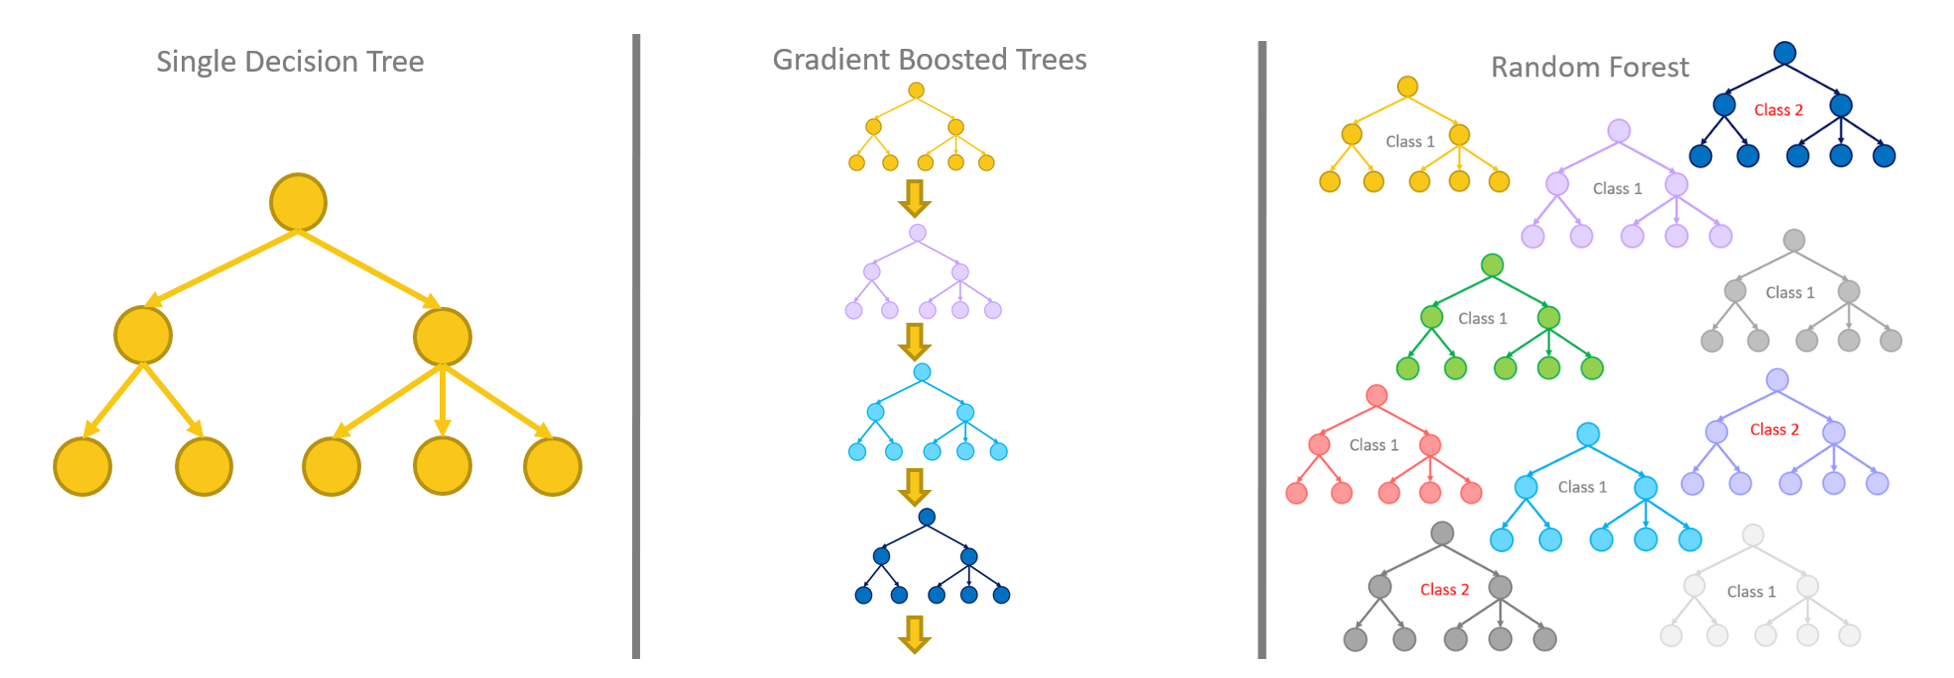
\includegraphics[width=1.15\textwidth]{trees.png}

\column{0.5\textwidth}
\centering
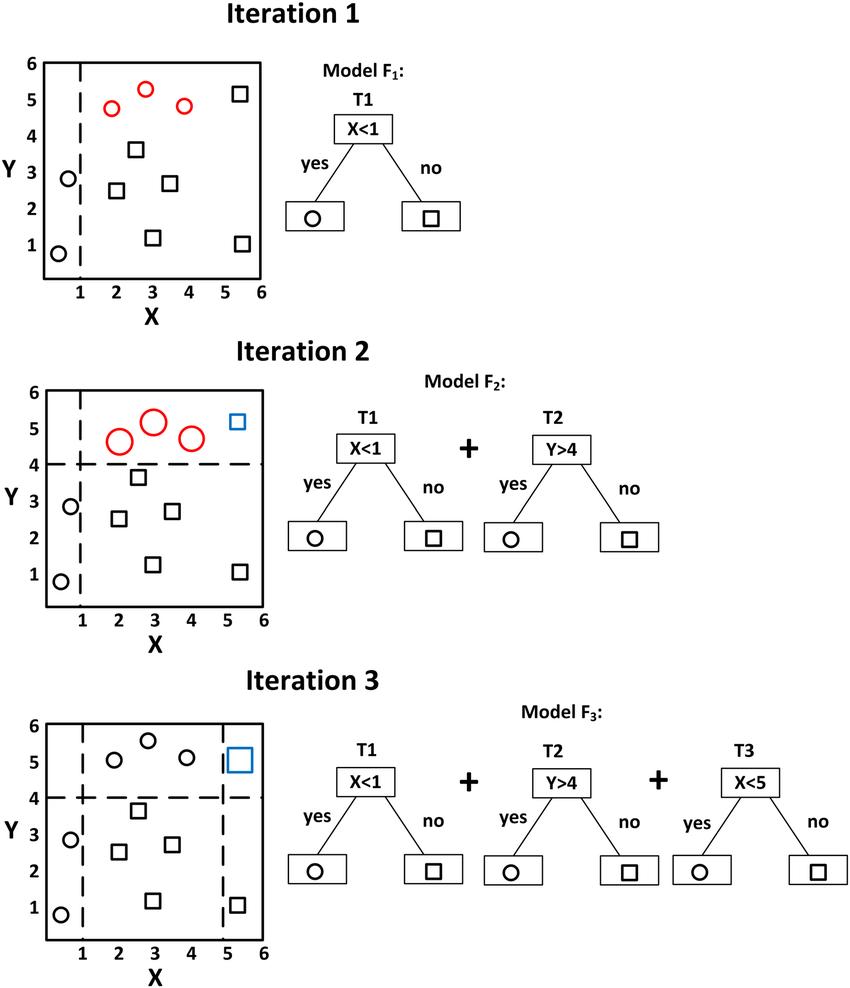
\includegraphics[width=0.8\textwidth]{gradient_boosting.png}
\end{columns}

\end{frame}

%------------------------------------------------
%------------------------------------------------
\section{Modelling nonlinearities}
%------------------------------------------------
%------------------------------------------------

\begin{frame}[plain]
\centering
\huge
%\begin{textblock*}{0.3\paperwidth}(0.25\paperwidth,0.3\paperheight)
\centering
\vspace{0.1\paperheight}
\begin{tcolorbox}[colframe=white, colback=mygrey, width=0.62\paperwidth,
arc=2.mm, boxsep=2mm,
box align=center,
halign=center,
valign=center,
]
\insertsection
\end{tcolorbox}
%\end{textblock*}
\transfade[duration=.4]
\end{frame}

%------------------------------------------------

\subsection{linear models}
\begin{frame}
\myframetitle{0.45\paperwidth}{0.04\paperwidth}{\insertsection}
\myframesubtitle{0.47\paperwidth}{\insertsubsection}
\centering
\vspace{0.2\paperheight}
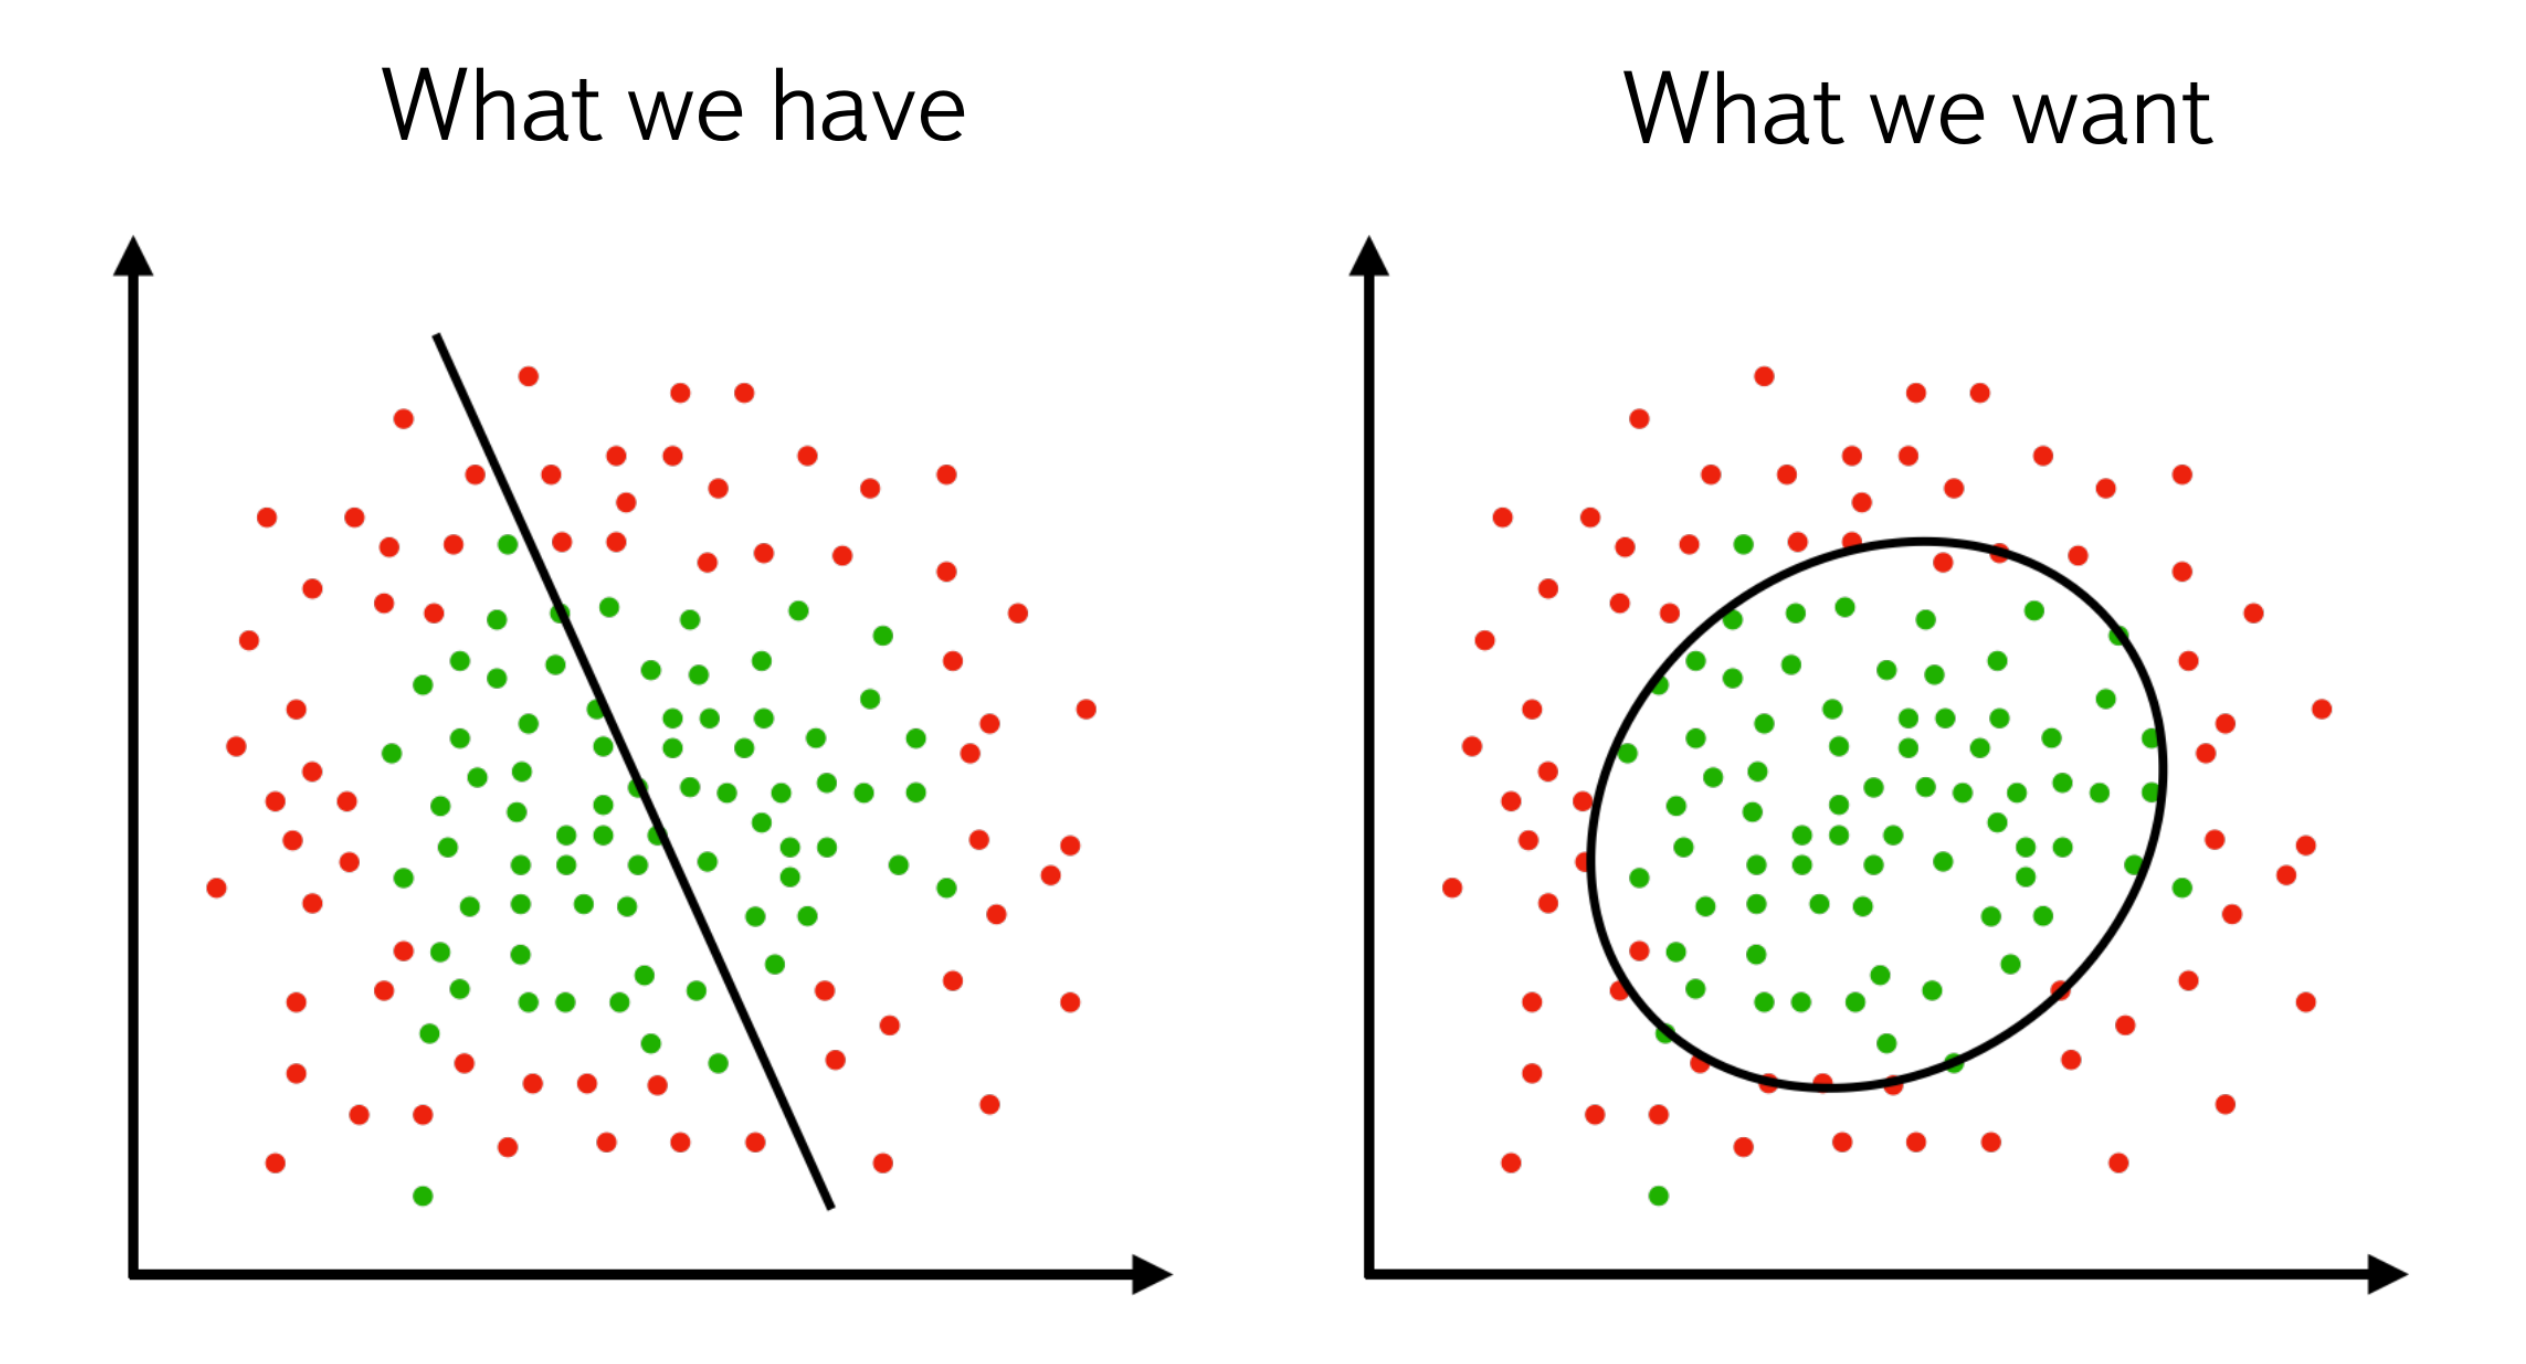
\includegraphics[width=0.6\linewidth]{want_have.png}\\

\centering
\footnotesize
\vspace{0.05\paperheight}
Linear models can't simply describe complex nonlinear data

\end{frame}

%------------------------------------------------

\subsection{trees}
\begin{frame}
\myframetitle{0.45\paperwidth}{0.04\paperwidth}{\insertsection}
\myframesubtitle{0.47\paperwidth}{\insertsubsection}

\vspace{0.15\paperheight}
\begin{columns}
\column{0.63\textwidth}
\begin{minipage}{\linewidth}
\begin{itemize}
	\small
	\setbeamertemplate{items}{\mybullet}
	\item (Ensembles of) Trees were designed to approximate nonlinearities and are \textbf{pretty good} in it + they are \textbf{fast and interpretable}
	\item But they are just "brute-force" algorithms -- \textbf{don't infer symmetries} in data by design
	\item \textbf{Ad-hoc, cut-based and piecewise approximations} of data at hand + not differentiable and smooth
\end{itemize}
\end{minipage}

\column{0.4\textwidth}
\begin{minipage}{\linewidth}
\centering
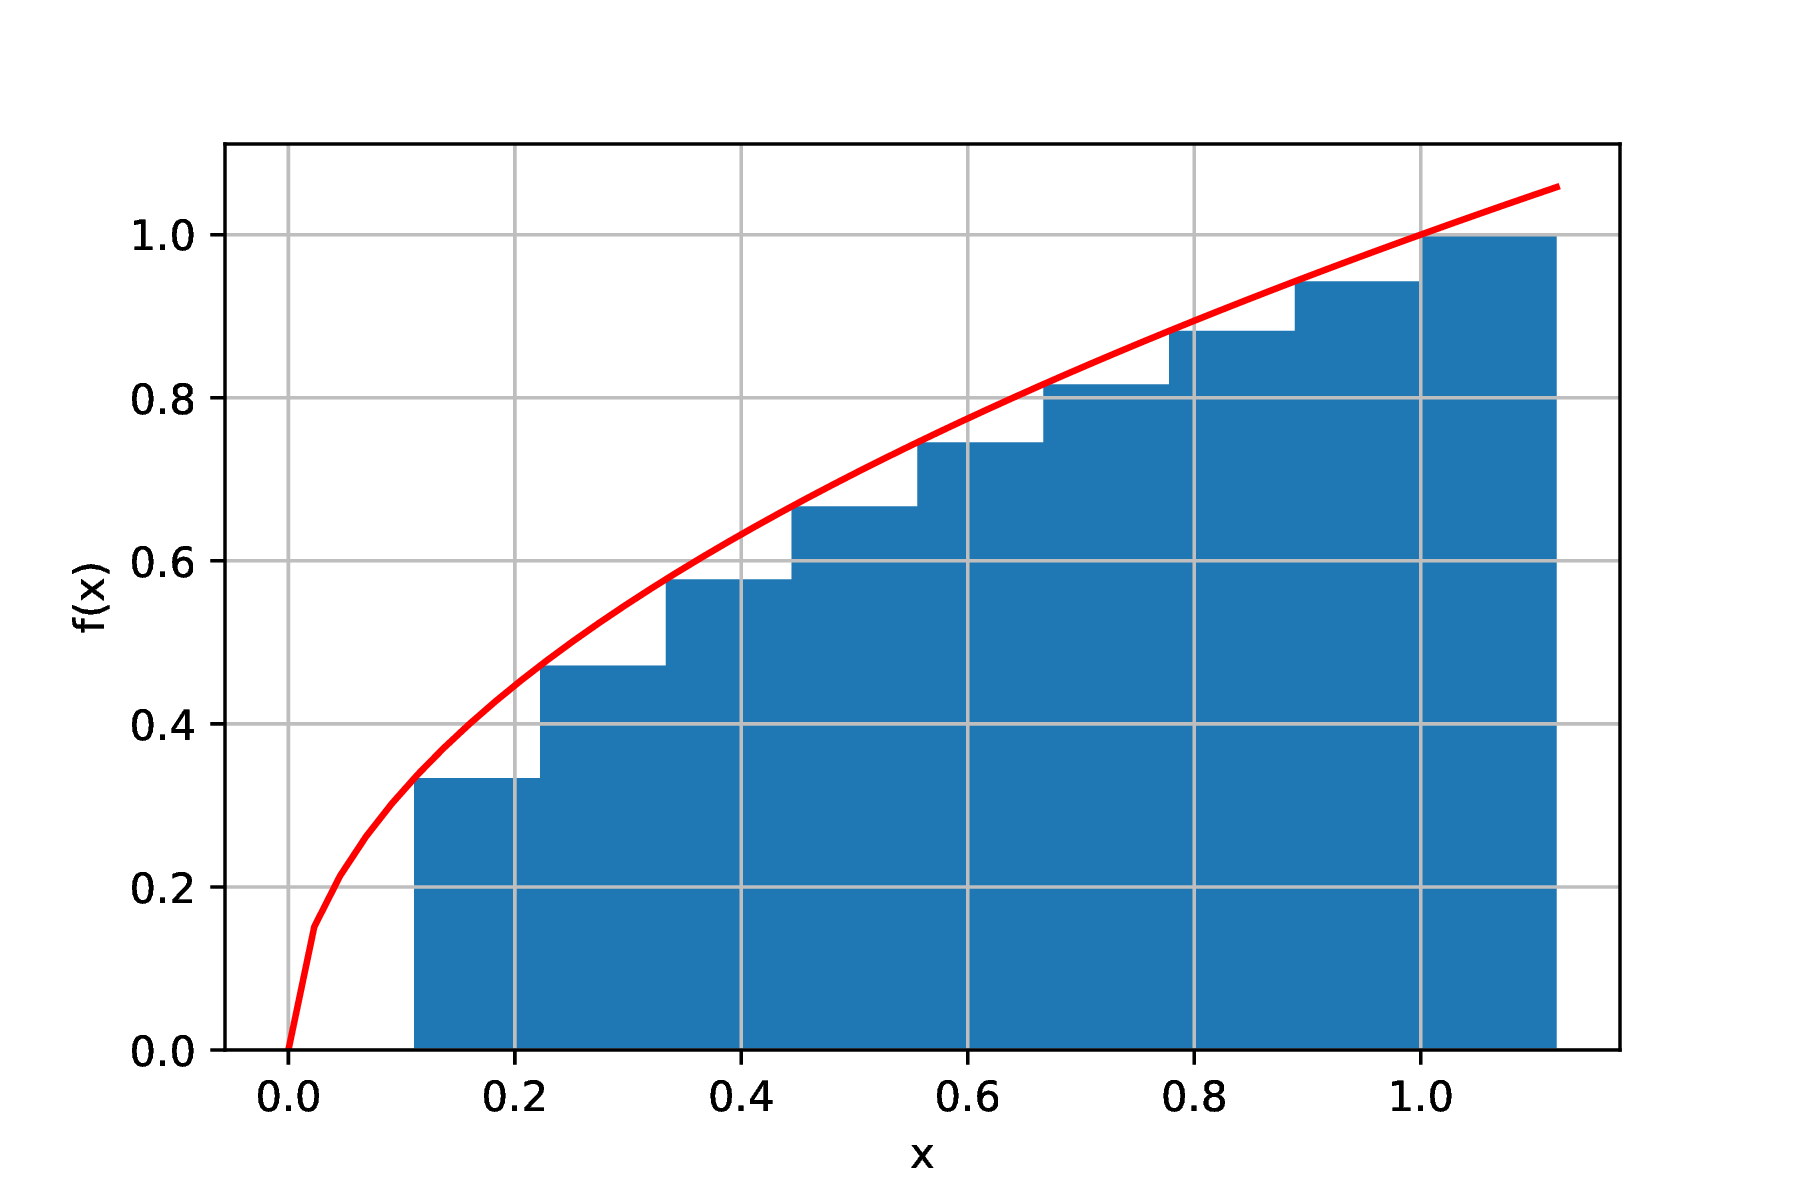
\includegraphics[width=0.8\linewidth]{plot.png}\\
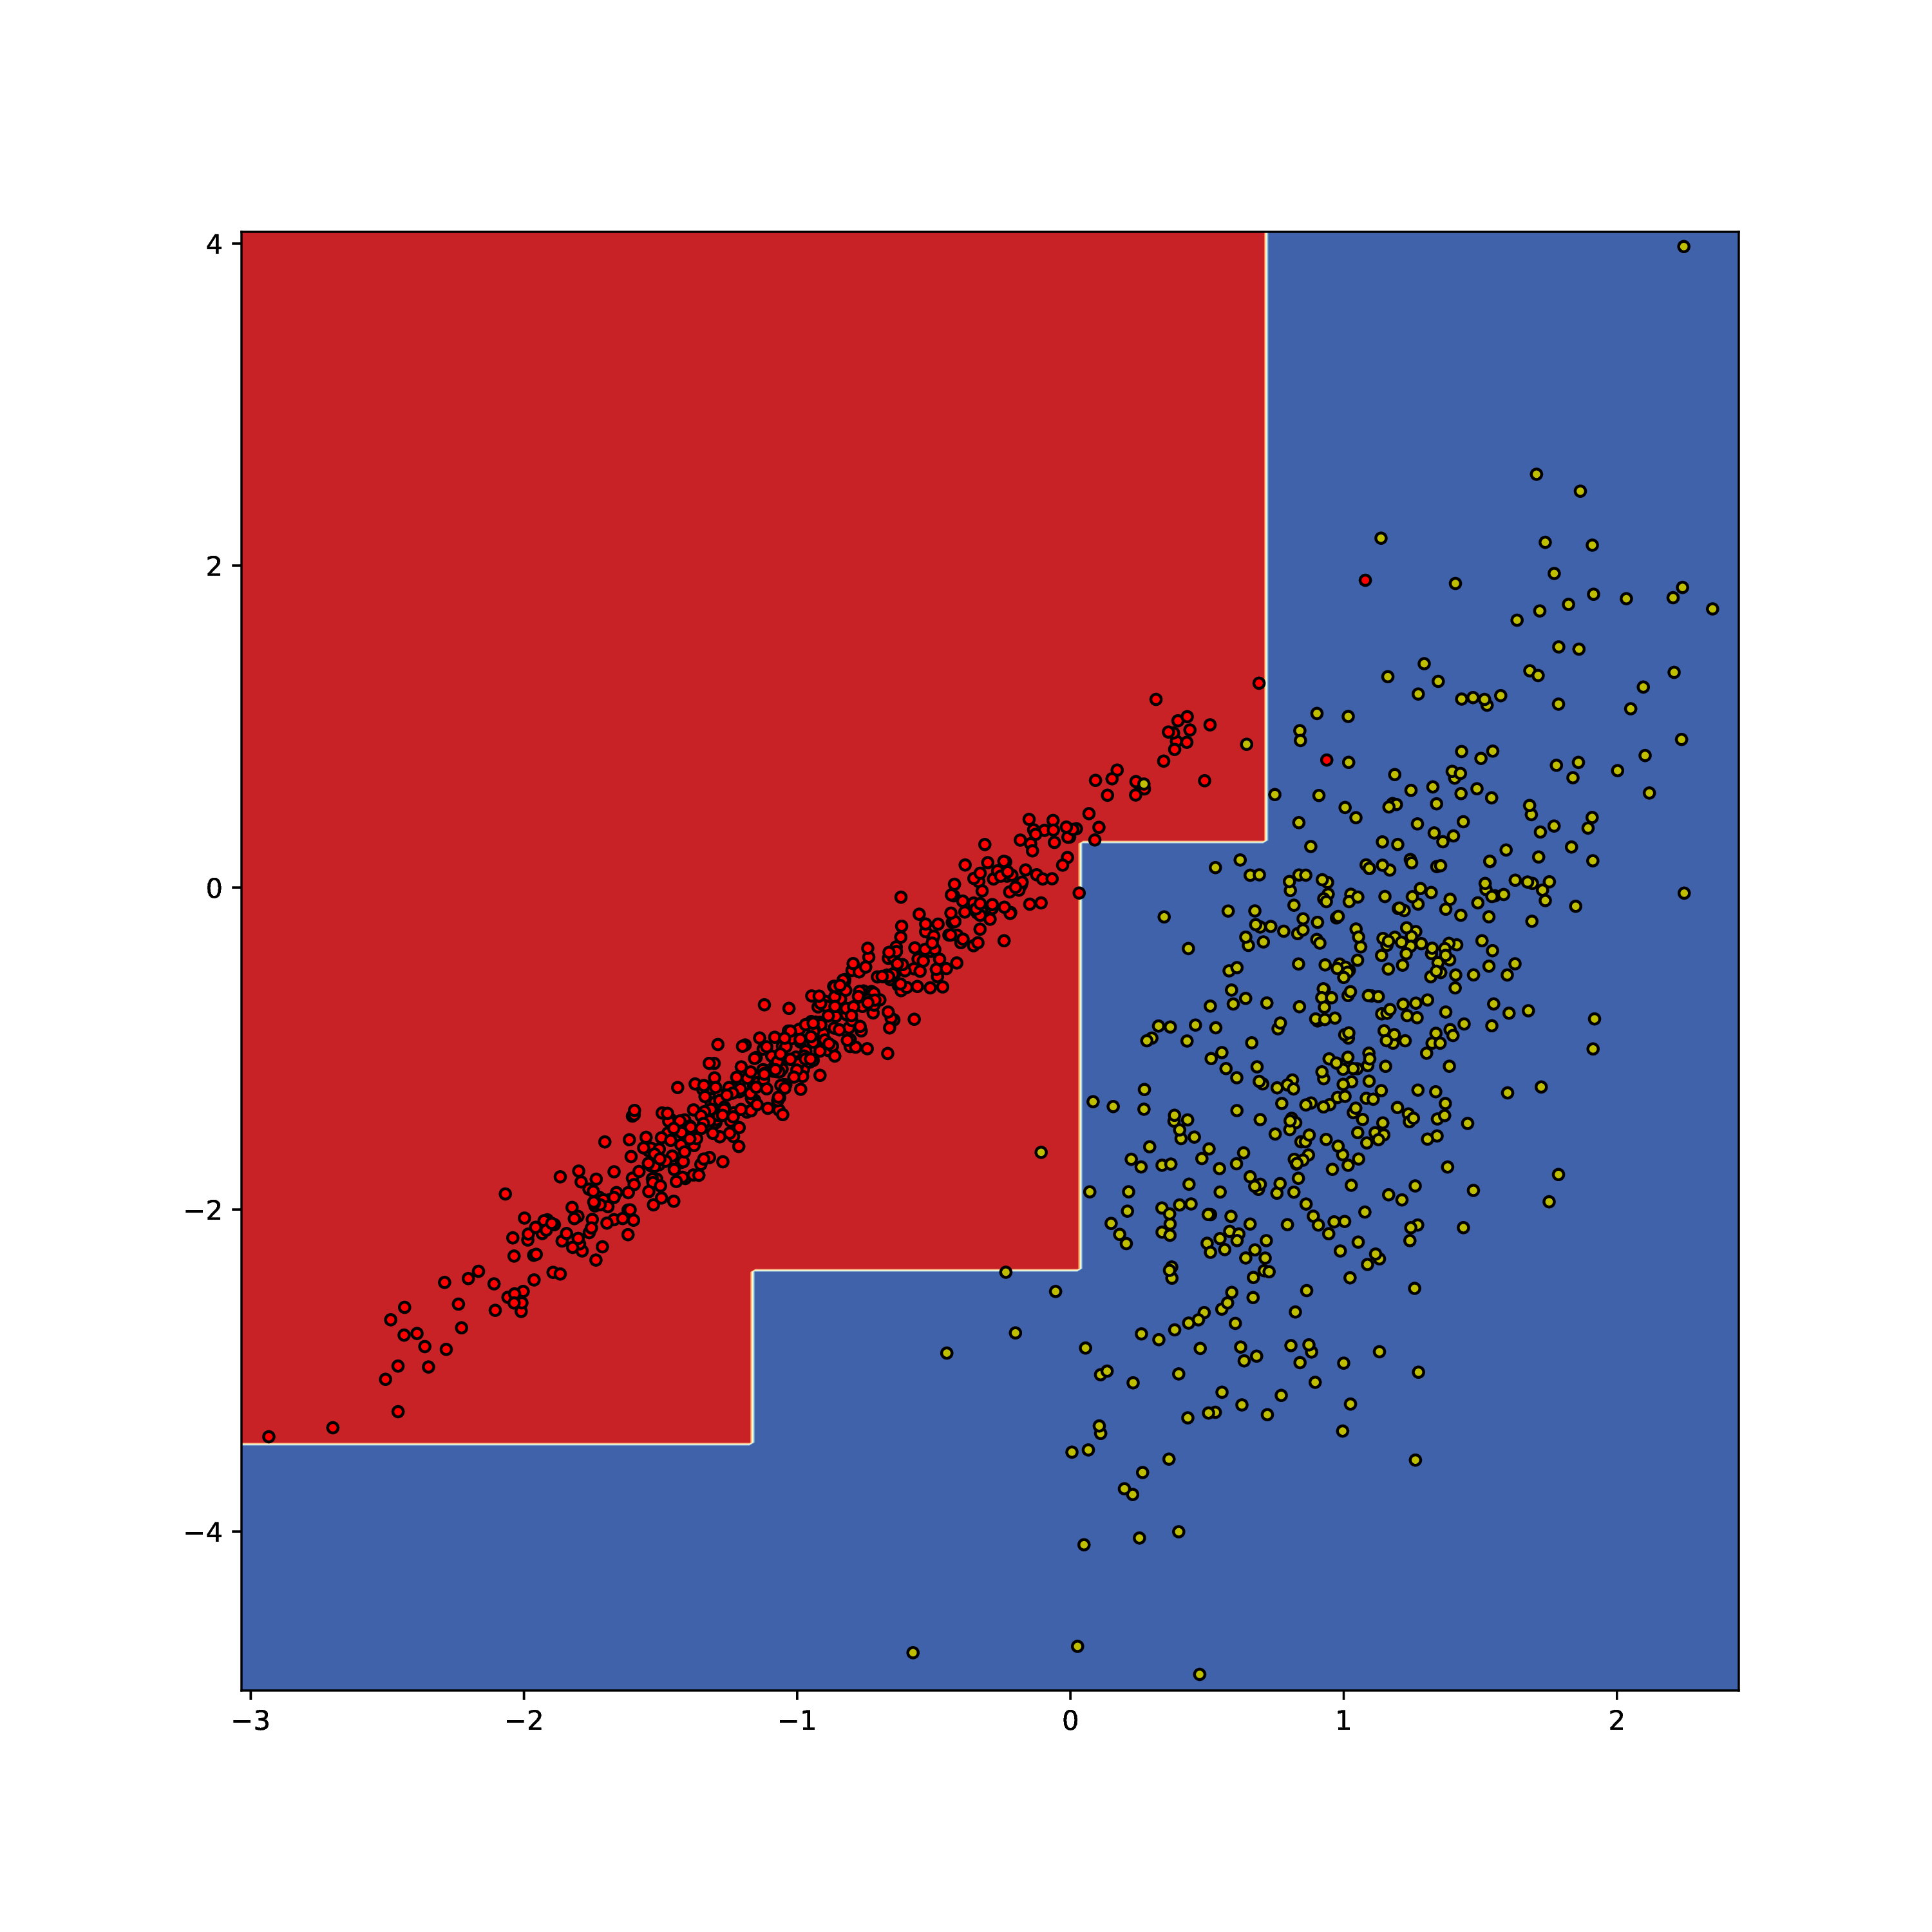
\includegraphics[width=0.8\linewidth]{4gi.png}\\
\end{minipage}
\end{columns}
\end{frame}

%------------------------------------------------

\subsection{feature engineering}
\begin{frame}
\myframetitle{0.45\paperwidth}{0.04\paperwidth}{\insertsection}
\myframesubtitle{0.47\paperwidth}{\insertsubsection}
\centering
\vspace{1.7cm}
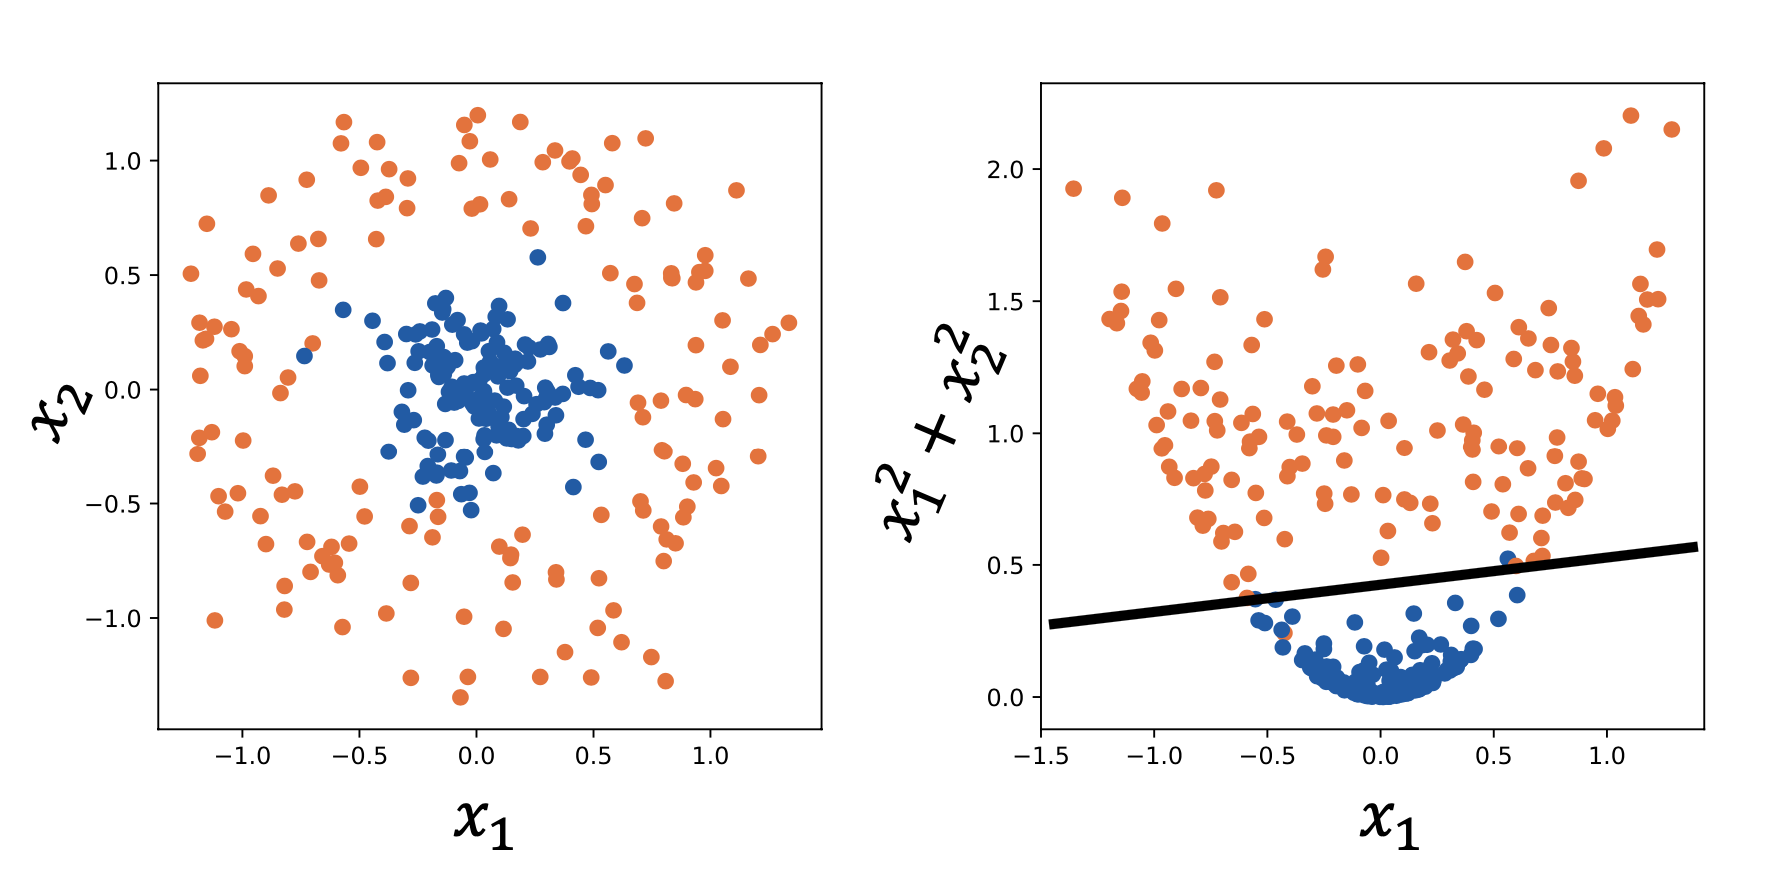
\includegraphics[width=0.5\linewidth]{feature_engin.png}\\
\begin{itemize}
	\small
	\setbeamertemplate{items}{\mybullet}
	\item But sometimes we know \textit{a priori} that there are transformations simplifying the problem $\rightarrow$ even linear model can do the job
	\item However, this \textbf{feature engineering} is non-trivial, requires domain knowledge and is time-consuming
\end{itemize}

\only<2->{
\begin{textblock*}{0.9\textwidth}(0.1\paperwidth, 0.89\paperheight)
	\centering
	\small
	\textcolor{myorange}{What if we design a model which could \textbf{automatically} feature-engineer itself?}
\end{textblock*}

}
\end{frame}

%------------------------------------------------
%------------------------------------------------
\section{Neural Network}
%------------------------------------------------
%------------------------------------------------

\begin{frame}[plain]
\centering
\huge
%\begin{textblock*}{0.3\paperwidth}(0.25\paperwidth,0.3\paperheight)
\centering
\vspace{0.1\paperheight}
\begin{tcolorbox}[colframe=white, colback=mygrey, width=0.5\paperwidth,
arc=2.mm, boxsep=2mm,
box align=center,
halign=center,
valign=center,
]
\insertsection
\end{tcolorbox}
%\end{textblock*}
\transfade[duration=.4]
\end{frame}

%------------------------------------------------

\subsection{automating FE}
\begin{frame}
\myframetitle{0.35\paperwidth}{0.04\paperwidth}{\insertsection}
\myframesubtitle{0.35\paperwidth}{\insertsubsection}
\centering

\vspace{0.6\paperheight}
\begin{textblock*}{0.5\paperwidth}(0.27\paperwidth, 0.25\paperheight)
	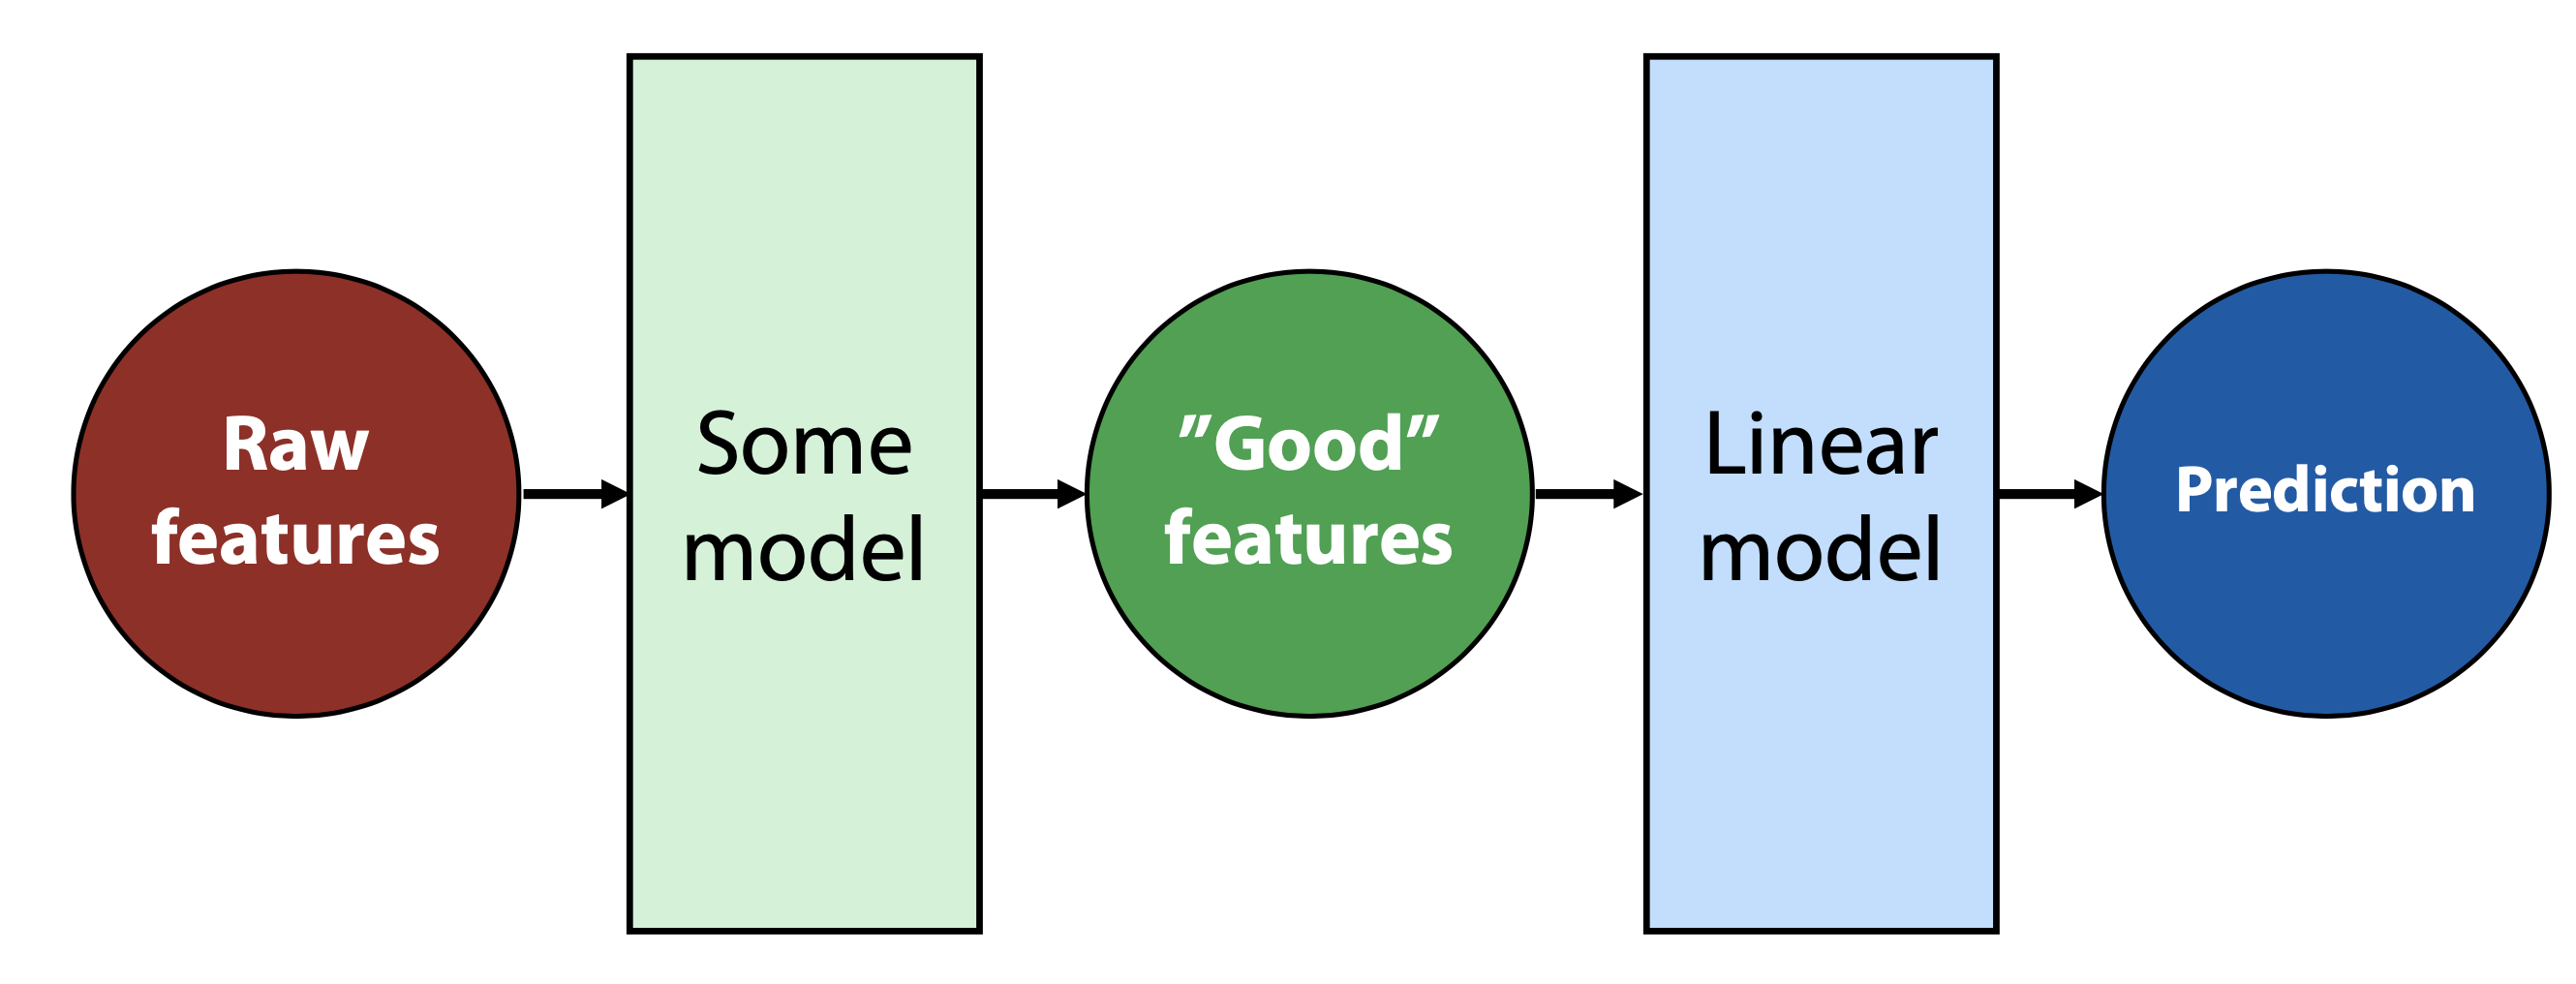
\includegraphics[width=1.\linewidth]{some_model.png}
\end{textblock*}

\vspace{0.02\paperheight}
\begin{itemize}
	\footnotesize
	\setbeamertemplate{items}{\mybullet}
	\item Let's use a \textbf{simple linear model} to solve our supervised problem 
	\item Add a block to a linear model which will automatically \textbf{generate new features} for it 
	\item Two blocks would work together as a \textbf{single model} $\Rightarrow$ their parameters are updated simultaneously
	\item And \textbf{automatically}, by e.g. gradient descent (given their differentiability)
\end{itemize}

\begin{textblock*}{0.25\paperwidth}(0.75\paperwidth,0.1\paperheight)
	\scriptsize
	\textcolor{gray}{NN illustrations from \href{https://indico.cern.ch/event/838377/}{\underline{ML in HEP 2020}}}
\end{textblock*}

\end{frame}

%------------------------------------------------

\begin{frame}
\myframetitle{0.35\paperwidth}{0.04\paperwidth}{\insertsection}
\myframesubtitle{0.35\paperwidth}{\insertsubsection}

\vspace{0.6\paperheight}
\begin{textblock*}{0.5\paperwidth}(0.27\paperwidth, 0.25\paperheight)
	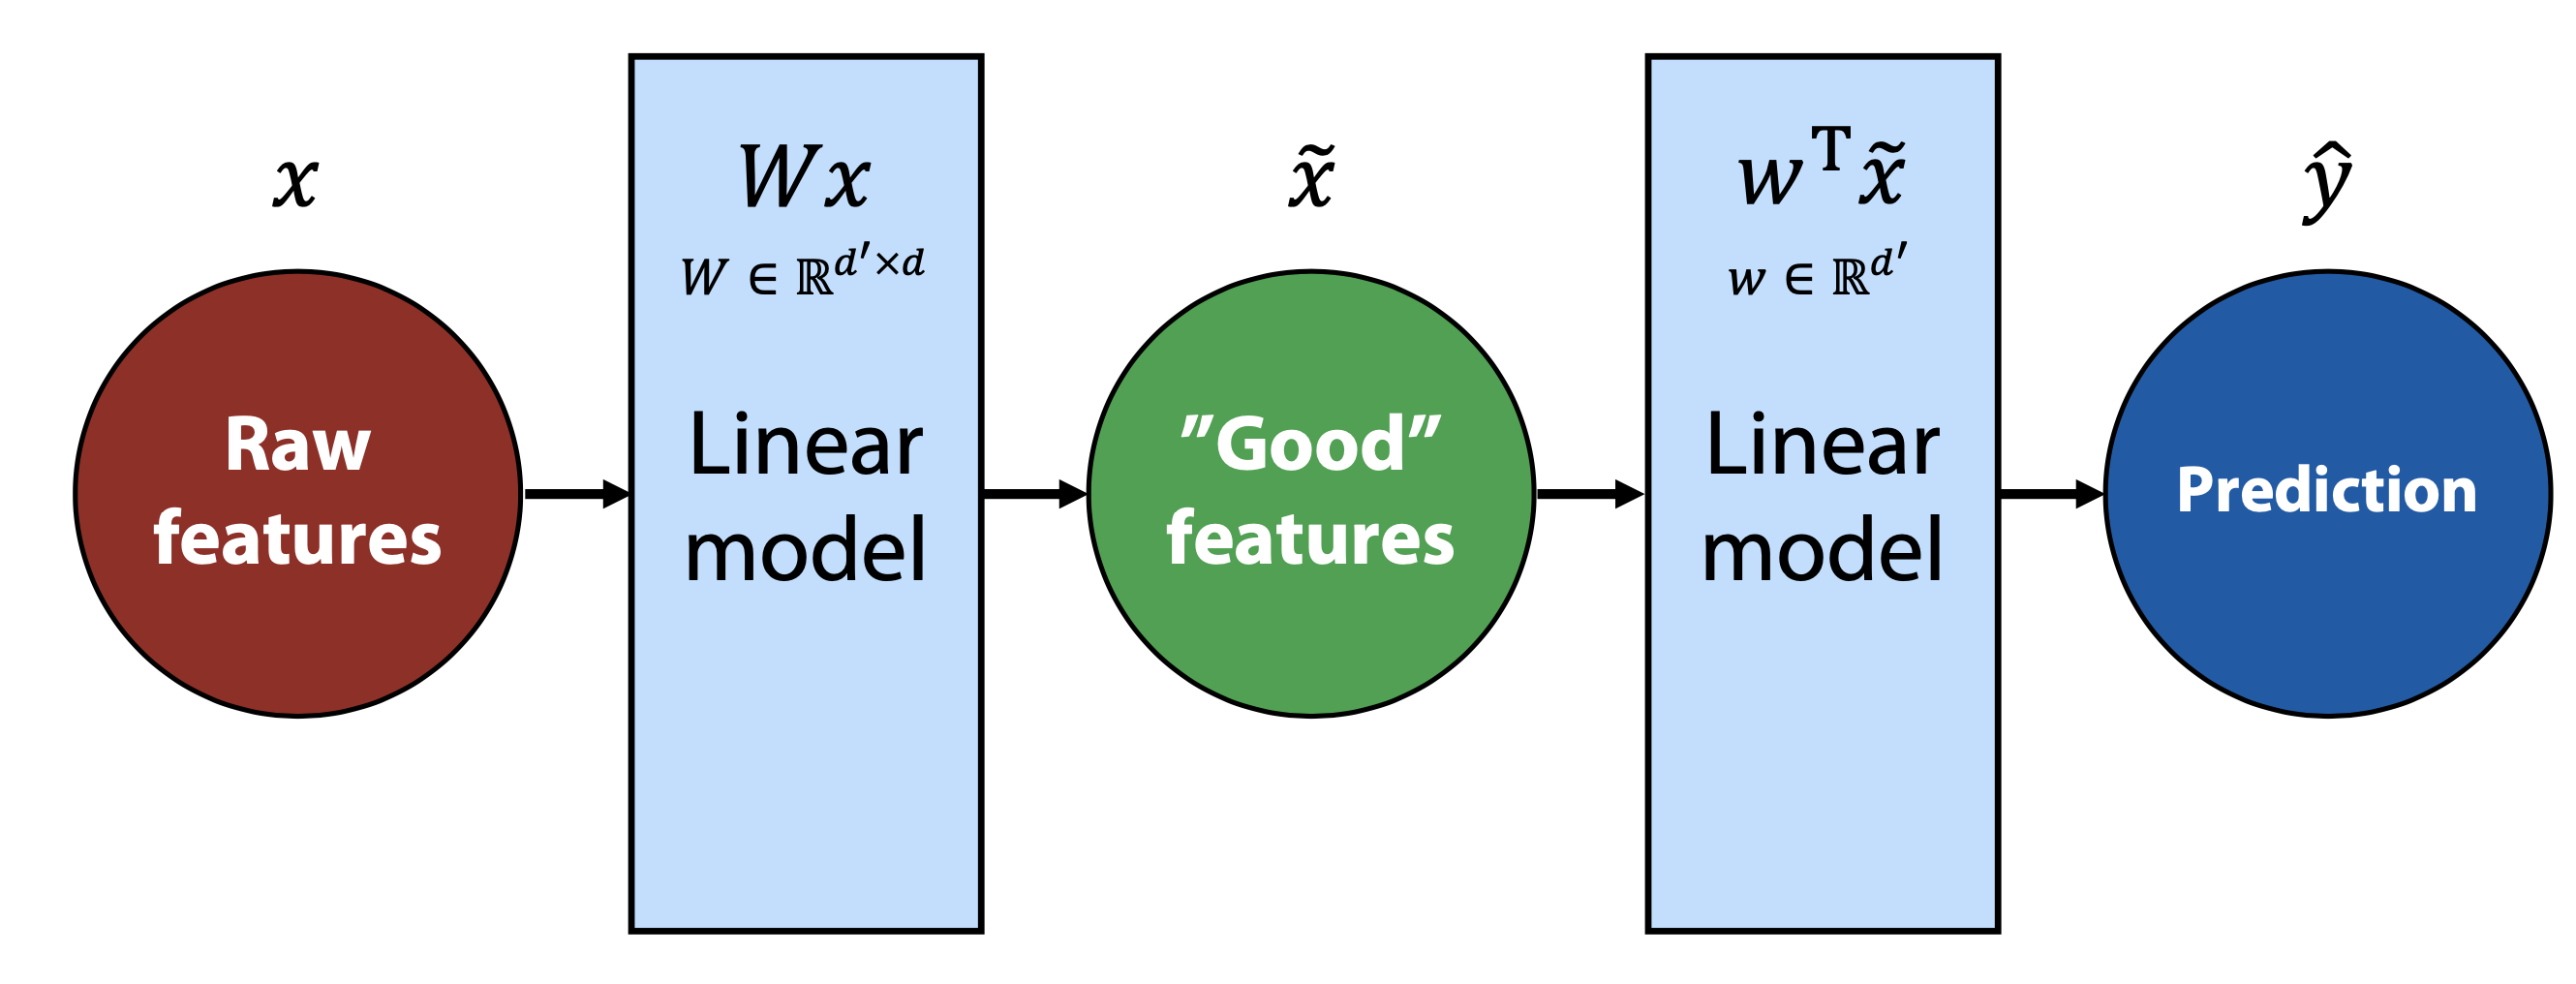
\includegraphics[width=1.\linewidth]{lin_model.png}
\end{textblock*}

\begin{itemize}
	\footnotesize
	\setbeamertemplate{items}{\mybullet}
	\item Would a linear model work as a feature generating model? \only<2->{\textcolor{myorange}{No}}
	\item<2> {$\hat{y} = w^{T}\tilde{x} = w^{T} (W x) = (w^{T} W) x = w'^{T} x \Rightarrow$ it is still a linear model}
	\item<2>[\textcolor{myorange}{\MVRightArrow}] \textcolor{myorange}{Input feature space has not changed, only the model weights}
\end{itemize}
\end{frame}

%------------------------------------------------

\begin{frame}
\myframetitle{0.35\paperwidth}{0.04\paperwidth}{\insertsection}
\myframesubtitle{0.35\paperwidth}{\insertsubsection}

\vspace{0.6\paperheight}
\begin{textblock*}{0.5\paperwidth}(0.27\paperwidth, 0.25\paperheight)
	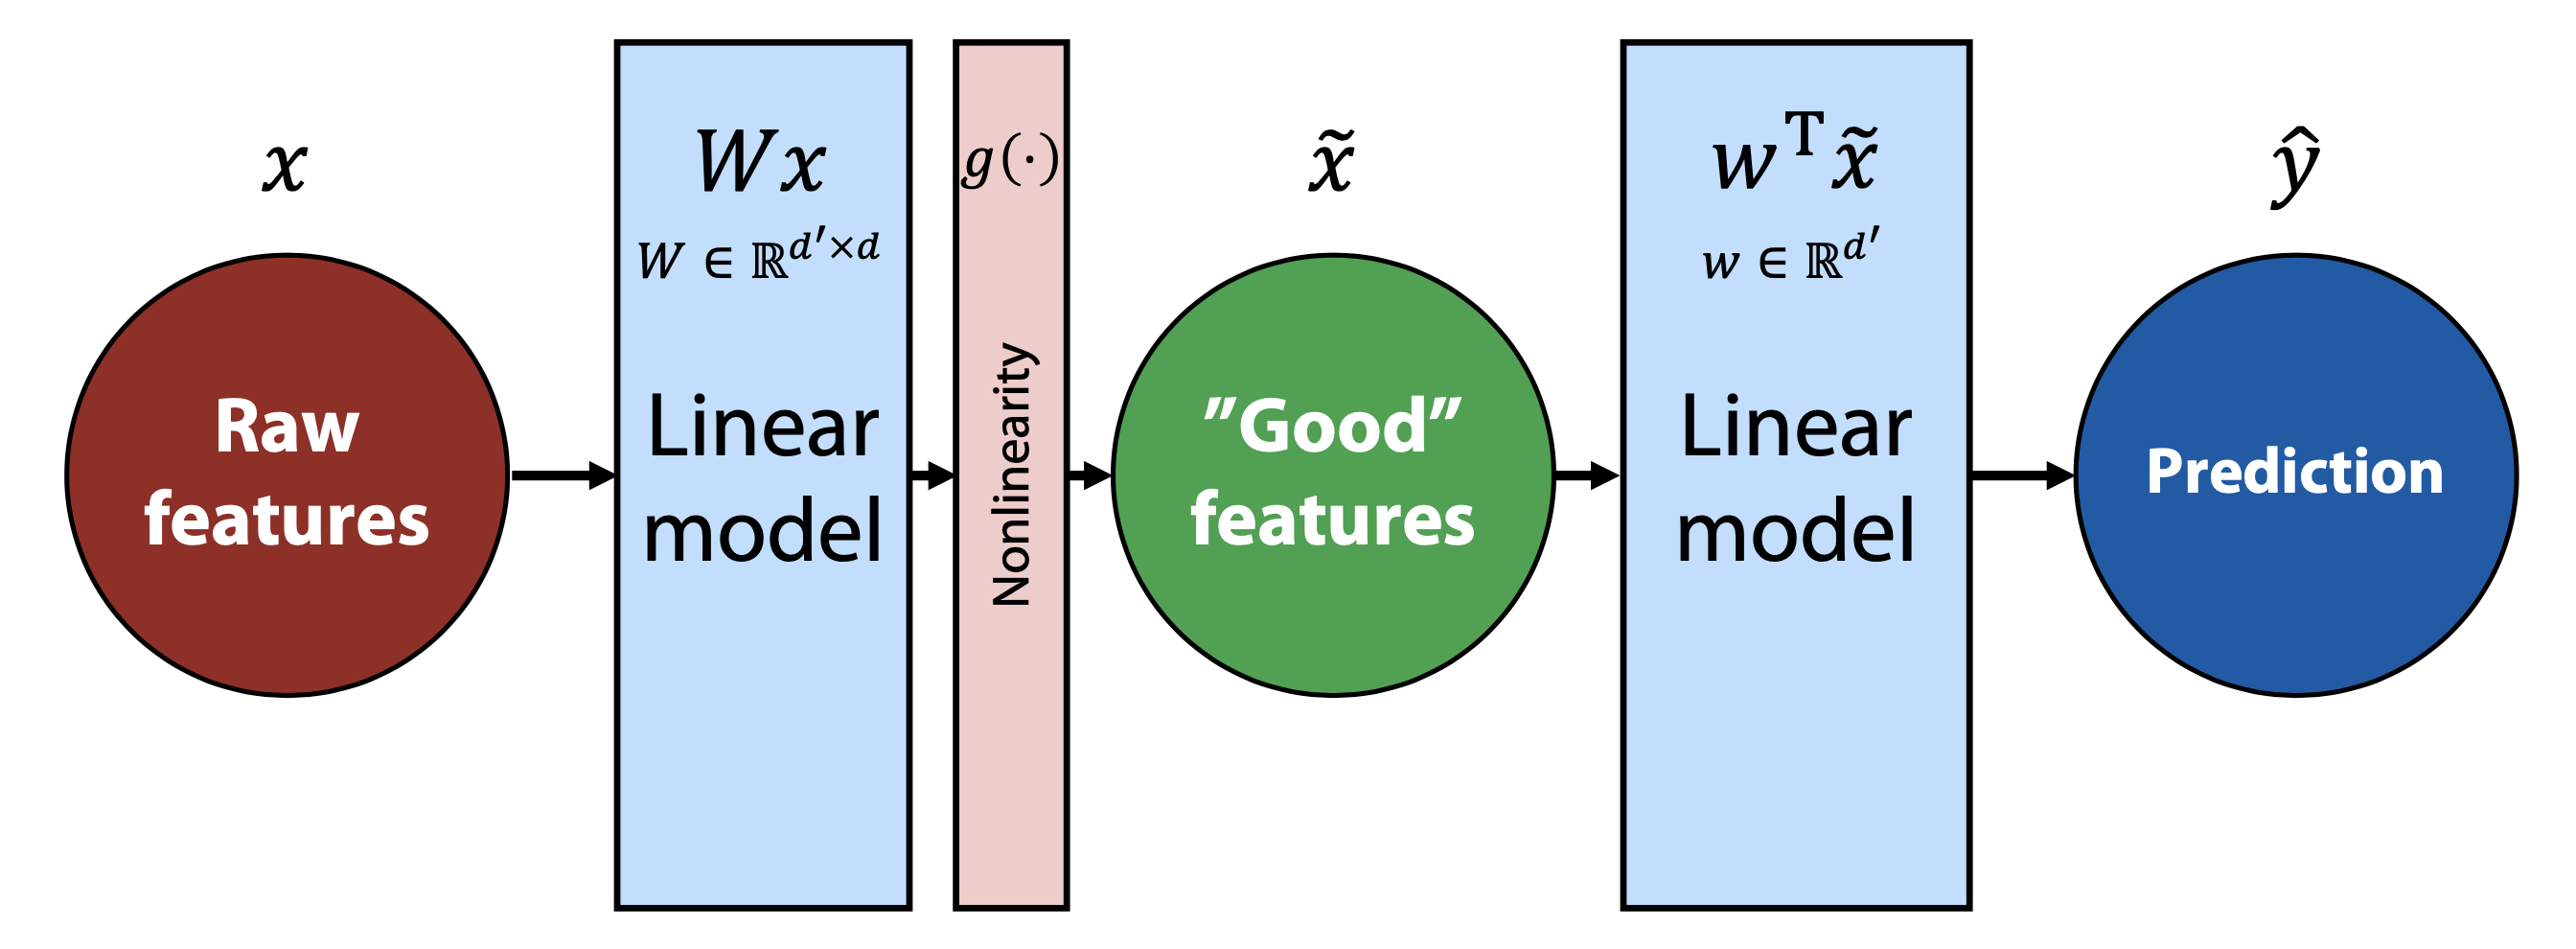
\includegraphics[width=1.\linewidth]{add_nonlin.png}
\end{textblock*}

\begin{itemize}
	\footnotesize
	\setbeamertemplate{items}{\mybullet}
	\item Let's then introduce \textbf{nonlinearity} to our model
	\item[\textcolor{myblack}{\MVRightArrow}] $\hat{y} = w^{T} \tilde{x} = w^{T} g(W x)$,\\
where $g(\cdot)$ -- some nonlinear scalar function (applied elementwise)
	\item<2->[\textcolor{myblack}{\MVRightArrow}] This is the simplest example of a \textcolor{myorange}{\textbf{neural network}}
\end{itemize}
\end{frame}

%------------------------------------------------

\subsection{architecture}
\begin{frame}
\myframetitle{0.35\paperwidth}{0.04\paperwidth}{\insertsection}
\myframesubtitle{0.35\paperwidth}{\insertsubsection}

\vspace{0.68\paperheight}
\begin{textblock*}{0.65\paperwidth}(0.21\paperwidth, 0.25\paperheight)
	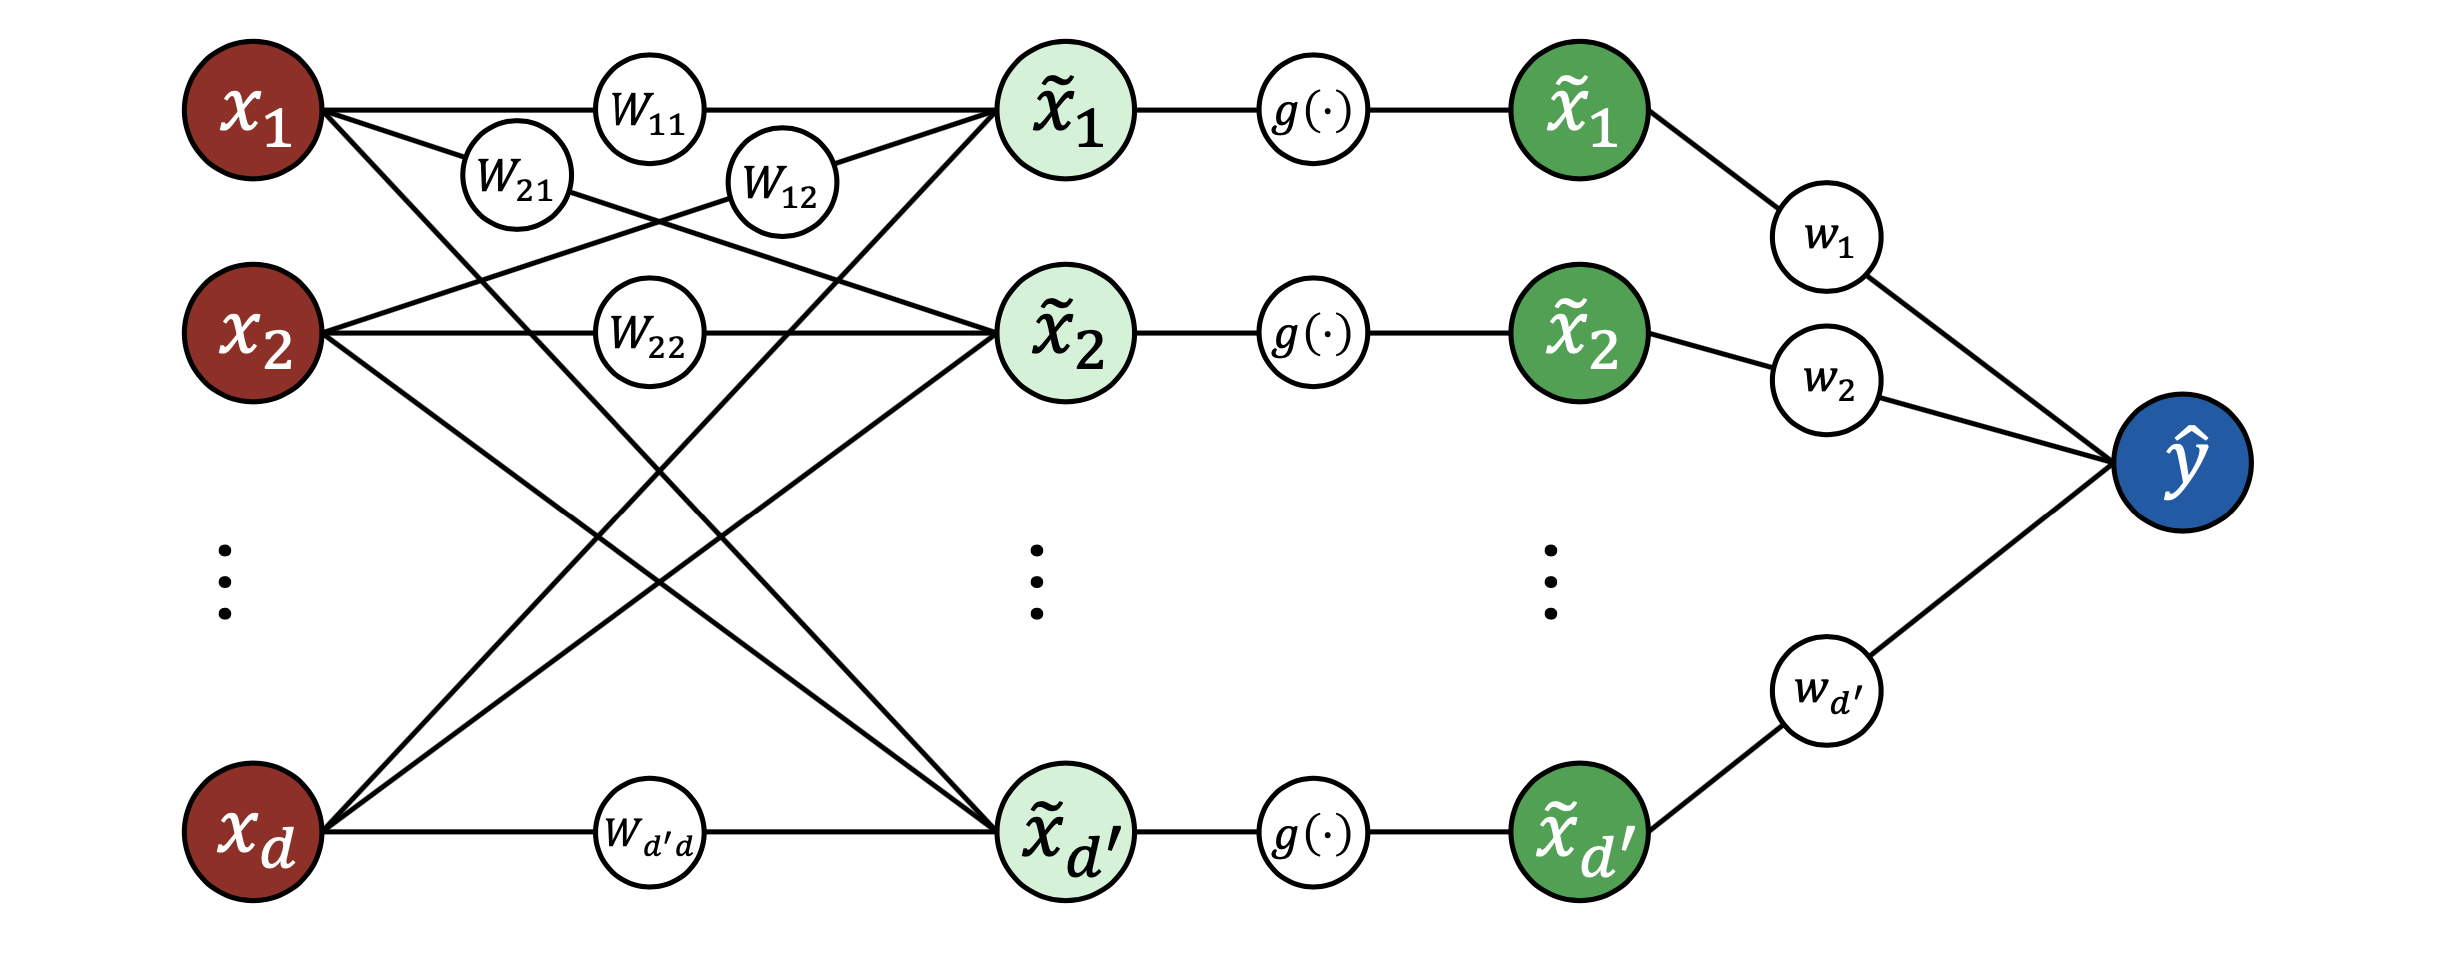
\includegraphics[width=1.\linewidth]{nn_details.png}
\end{textblock*}

\begin{itemize}
\centering
\small
\setbeamertemplate{items}{\mybullet}
\item[] Essentially, NN is just a \textbf{composite function} that maps a set of $X$ to a set of $Y$
\item[] $\hat{y} = w^{T} \tilde{x} = w^{T} g(W x)$
\end{itemize}
\end{frame}

%------------------------------------------------

\subsection{terminology}
\begin{frame}
\myframetitle{0.35\paperwidth}{0.04\paperwidth}{\insertsection}
\myframesubtitle{0.35\paperwidth}{\insertsubsection}
\centering
\vspace{2.cm}

\begin{columns}
	
\column{0.4\textwidth}
\begin{minipage}{\linewidth}
\begin{center}
\textbf{Feed-forward network:}\\
\hfill \break
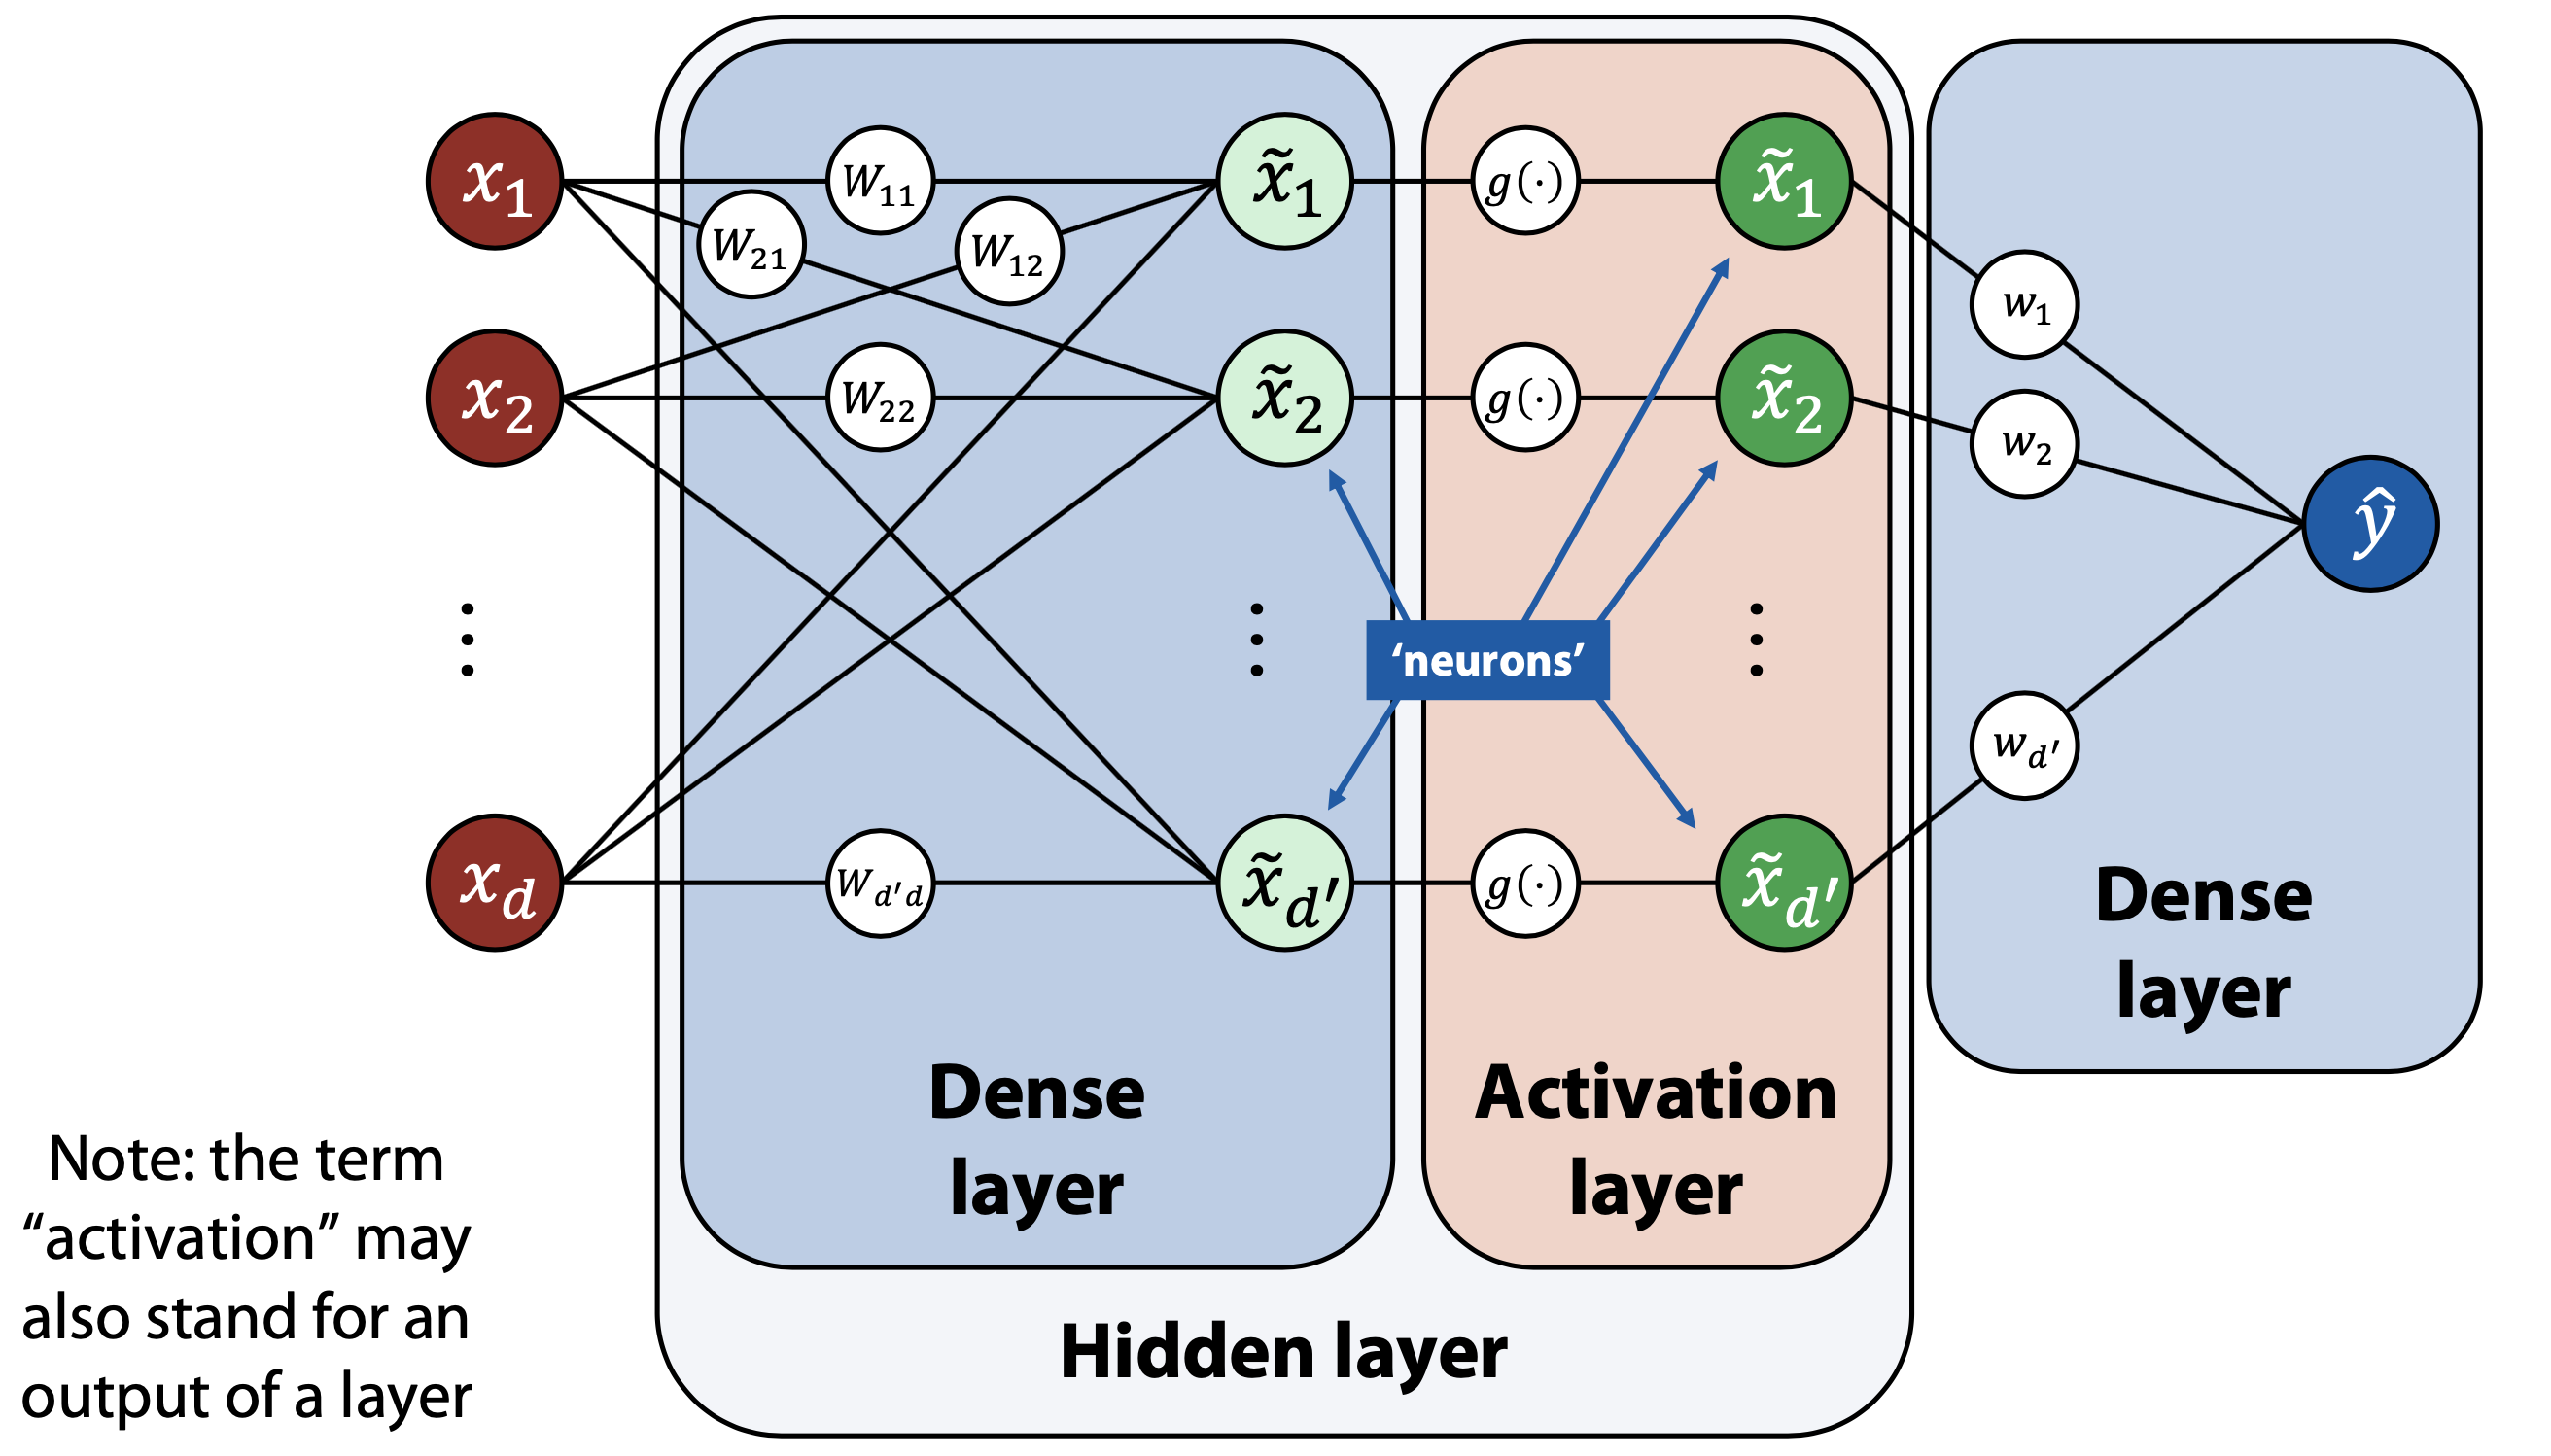
\includegraphics[width=1.0\linewidth]{nn_terminology.png}
\end{center}
\end{minipage}

\column{0.7\textwidth}
\begin{minipage}{\linewidth}
\begin{itemize}
	\small
	\itemsep1.ex
	\setbeamertemplate{items}{\mybullet}
	\item {\textcolor{Brown}{Brown} nodes $x_{1}, x_{2}, ..., x_{d}$ -- features from an \textbf{input layer}}
	\item {\textcolor{mygreen}{Green} nodes $\tilde{x}_{1}, \tilde{x}_{2}, ..., \tilde{x}_{d\prime}$-- \textbf{neurons} from a \textbf{hidden layer}}
	\item {\textcolor{MidnightBlue}{Blue} node $\hat{y}$ -- neuron from an \textbf{output layer}}
	\item {Straight lines (edges) between neurons -- \textbf{weights} $w_{ij}$}
	\item {$g(\cdot)$ -- nonlinear \textbf{activation} function, e.g. sigmoid $\sigma(\cdot)$}
	\item {\textcolor{myorange}{Important:} each neuron has additional \textbf{bias} $b$ associated to it and added to other inputs (not illustrated)}
\end{itemize}
\end{minipage}
\end{columns}

\end{frame}

%------------------------------------------------

\subsection{human brain}
\begin{frame}
\myframetitle{0.35\paperwidth}{0.04\paperwidth}{\insertsection}
\myframesubtitle{0.35\paperwidth}{\insertsubsection}

\centering
\vspace{0.25\paperheight}
\includegraphics[width=.9\linewidth]{brain.png}
\vspace{0.07\paperheight}
\centering
\small
%Furthermore, one can think of NN as of something resembling neurons in human brain
%Neurons on human brain consist of a nucleus, dendrites, cell body, and axon. The number of neurons in humans is approximately 140 billion, consist of 100 billion neurons and 40 billion synapses in neurons.
\end{frame}

%------------------------------------------------
%------------------------------------------------
\section{Training}
%------------------------------------------------
%------------------------------------------------

\begin{frame}[plain]
\centering
\huge
%\begin{textblock*}{0.3\paperwidth}(0.25\paperwidth,0.3\paperheight)
\centering
\vspace{0.1\paperheight}
\begin{tcolorbox}[colframe=white, colback=mygrey, width=0.3\paperwidth,
arc=2.mm, boxsep=2mm,
box align=center,
halign=center,
valign=center,
]
\insertsection
\end{tcolorbox}
%\end{textblock*}
\transfade[duration=.4]
\end{frame}

%------------------------------------------------

\subsection{how to train?}
\begin{frame}
\myframetitle{0.22\paperwidth}{0.04\paperwidth}{\insertsection}
\myframesubtitle{0.23\paperwidth}{\insertsubsection}
\vspace{0.2\paperheight}

\begin{itemize}
	\small
\setbeamertemplate{items}{\mybullet}
\item Since NN fundamentally is a parametrized differentiable model we can optimise the loss function and use \textbf{gradient descent} to train it:
\[
\bm\omega_{k+1} \leftarrow \bm\omega_{k} - \eta \cdot \textcolor{mypurple}{\nabla Q (\bm\omega_{k})}
\]
\item But \textcolor{mypurple}{gradients} are hard to derive analytically -- writing down all the derivatives is tough and tedious (especially for large NN) 
\item Note that NN is just a \textbf{composite model} $\Rightarrow$ can use \textbf{chain rule} for differentiating it
\end{itemize}

\end{frame}

%------------------------------------------------

\subsection{chain rule}
\begin{frame}
\myframetitle{0.22\paperwidth}{0.04\paperwidth}{\insertsection}
\myframesubtitle{0.23\paperwidth}{\insertsubsection}
\vspace{0.05\paperheight}

\begin{itemize}
	\small
\setbeamertemplate{items}{\mybullet}
\item Computing derivative of a "base" function is simple $\Rightarrow$ decompose composite function into a set of base ones and differentiate them one by one
\item Let's recall the rule:
\[
	\cfrac{\partial f \big(t(x) \big) }{\partial x} = \cfrac{\partial f(t)}{\partial t} \cdot \cfrac{\partial t(x)}{\partial x}
\]

\item[] \textcolor{myorange}{Exercise:} can you compute derivative of sigmoid function by decomposing it into base functions?
\[
\sigma(x) = \cfrac{1}{1+e^{-x}}
\]
\end{itemize}

\begin{textblock*}{0.9\linewidth}(0.15\paperwidth, 0.68\paperheight)
		\small
		\only<2->{
		\[
		\sigma(x) = f(g(h(p(x)))), \quad f(z) = \frac{1}{z}, \quad g(z) = 1+z, \quad  h(z) = e^{z}, \quad p(z) = -z
		\]
		\only<3->{
		\[
		\sigma'(x) = \cfrac{\partial f}{\partial g} \cdot \cfrac{\partial g}{\partial h} \cdot \cfrac{\partial h}{\partial p} \cdot \cfrac{\partial p}{\partial x} = -\cfrac{1}{g^2}\cdot 1 \cdot e^p \cdot (-1) = ... = \sigma(x) \cdot \big( 1 - \sigma(x) \big)
		\]
	}
	}
\end{textblock*}
\end{frame}

%------------------------------------------------

\subsection{backpropagation}
\begin{frame}
\myframetitle{0.22\paperwidth}{0.04\paperwidth}{\insertsection}
\myframesubtitle{0.23\paperwidth}{\insertsubsection}
\centering
\vspace{1.7cm}

\includegraphics[width=0.45\linewidth]{train_1.png}\\
\begin{itemize}
	\small
\setbeamertemplate{items}{\mybullet}
%\item So we know how to update weights
\item So how to find partial derivatives of loss function with respect to some weight?
\end{itemize}

\begin{textblock*}{0.35\paperwidth}(0.65\paperwidth,0.1\paperheight)
	\footnotesize
	\textcolor{gray}{backprop illustrations from \href{https://github.com/data-mining-in-action/}{\underline{DMIA}}}
\end{textblock*}

\end{frame}

%------------------------------------------------

\begin{frame}
\myframetitle{0.22\paperwidth}{0.04\paperwidth}{\insertsection}
\myframesubtitle{0.23\paperwidth}{\insertsubsection}
\centering
\vspace{2.cm}
\includegraphics[width=0.8\linewidth]{train_2.png}
\vspace{5mm}
\begin{itemize}
	\small
\setbeamertemplate{items}{\mybullet}
\item Let's consider a simplified neural network
\item Represent it in the form of a \textbf{computational graph}
\end{itemize}

\begin{textblock*}{0.35\paperwidth}(0.65\paperwidth,0.1\paperheight)
	\footnotesize
	\textcolor{gray}{backprop illustrations from \href{https://github.com/data-mining-in-action/}{\underline{DMIA}}}
\end{textblock*}
\end{frame}

%------------------------------------------------

\begin{frame}
\myframetitle{0.22\paperwidth}{0.04\paperwidth}{\insertsection}
\myframesubtitle{0.23\paperwidth}{\insertsubsection}
\centering
\vspace{2.3cm}
\includegraphics[width=0.8\linewidth]{train_3.png}\\
%\begin{itemize}
%\item {We know how to update a weight}
%\end{itemize}
\end{frame}

%------------------------------------------------

\begin{frame}
\myframetitle{0.22\paperwidth}{0.04\paperwidth}{\insertsection}
\myframesubtitle{0.23\paperwidth}{\insertsubsection}
\centering
\vspace{2.3cm}
\includegraphics[width=0.8\linewidth]{train_4.png}\\
%\begin{itemize}
%\item {We know how to find the partial derivative of the loss function with respect to some weight}
%\end{itemize}
\end{frame}

%------------------------------------------------

\begin{frame}
\myframetitle{0.22\paperwidth}{0.04\paperwidth}{\insertsection}
\myframesubtitle{0.23\paperwidth}{\insertsubsection}
\centering
\vspace{2.3cm}
\includegraphics[width=0.8\linewidth]{train_5.png}\\
%\begin{itemize}
%\item {Let's try to apply our knowledge to this simple neural network}
%\end{itemize}
\end{frame}

%------------------------------------------------

\begin{frame}
\myframetitle{0.22\paperwidth}{0.04\paperwidth}{\insertsection}
\myframesubtitle{0.23\paperwidth}{\insertsubsection}
\centering
\vspace{2.3cm}
\includegraphics[width=0.8\linewidth]{train_6.png}\\
%\begin{itemize}
%\item {Going back over the network to the beginning}
%\end{itemize}
\end{frame}

%------------------------------------------------

\begin{frame}
\myframetitle{0.22\paperwidth}{0.04\paperwidth}{\insertsection}
\myframesubtitle{0.23\paperwidth}{\insertsubsection}
\centering
\vspace{2.3cm}
\includegraphics[width=0.8\linewidth]{train_7.png}\\
%\begin{itemize}
%\item {Let's go further to the beginning}
%\end{itemize}
\end{frame}

%------------------------------------------------

\begin{frame}
\myframetitle{0.22\paperwidth}{0.04\paperwidth}{\insertsection}
\myframesubtitle{0.23\paperwidth}{\insertsubsection}
\centering
\vspace{2.3cm}
\includegraphics[width=0.8\linewidth]{train_8.png}\\
%\begin{itemize}
%\item {Now we know the value of the partial derivative of the loss function with respect to some weight}
%\end{itemize}

\begin{textblock*}{0.55\linewidth}(0.5\paperwidth, 0.68\paperheight)
	\small
	\only<2->{
	\begin{itemize}
		\footnotesize
		\item this procedure is called \textbf{backpropagation}
		\item its idea is to \textbf{collect derivatives} at each step in the computational graph w/o recalculating them every single time for every weight
	\end{itemize}
	}
\end{textblock*}

\end{frame}

%------------------------------------------------

\subsection{wrap it up}
\begin{frame}
\myframetitle{0.22\paperwidth}{0.04\paperwidth}{\insertsection}
\myframesubtitle{0.23\paperwidth}{\insertsubsection}
\centering
\vspace{0.61\paperheight}
\begin{textblock*}{0.8\textwidth}(0.1\paperwidth, 0.2\paperheight)
	\includegraphics<1>[width=0.8\linewidth]{train_9.png}
	\includegraphics<2>[width=0.8\linewidth]{train_10.png}
	\includegraphics<3>[width=0.8\linewidth]{train_3.png}
	\includegraphics<4->[width=0.8\linewidth]{train_9.png}
\end{textblock*}


\begin{enumerate}
	\footnotesize
	\item<1-> make \textbf{forward pass} through NN to calculate the output of each neuron and value of loss function
	\item<2-> with \textbf{backward pass} go back through NN to calculate gradients for all weights
	\item<3-> update weights with their gradients
	\item<4-> repeat until convergence
	\item<4->[] *one iteration (\textbf{epoch}) = forward and backward pass
\end{enumerate}

\begin{textblock*}{0.45\paperwidth}(0.6\paperwidth,0.1\paperheight)
	\footnotesize
	\href{https://playground.tensorflow.org/}{\textcolor{gray}{\underline{train NN in your browser!}}}
\end{textblock*}

\end{frame}

%------------------------------------------------
%------------------------------------------------
\section{Summary}
%------------------------------------------------
%------------------------------------------------

\begin{frame}[plain]
\centering
\huge
%\begin{textblock*}{0.3\paperwidth}(0.25\paperwidth,0.3\paperheight)
\centering
\vspace{0.1\paperheight}
\begin{tcolorbox}[colframe=white, colback=mygrey, width=0.3\paperwidth,
arc=2.mm, boxsep=2mm,
box align=center,
halign=center,
valign=center,
]
\insertsection
\end{tcolorbox}
%\end{textblock*}
\transfade[duration=.4]
\end{frame}

%------------------------------------------------

\begin{frame}
\myframetitle{0.25\paperwidth}{0.04\paperwidth}{\insertsection}
%\myframesubtitle{0.41\paperwidth}{\insertsubsection}

\vspace{0.2\paperheight}
\begin{itemize}
	\itemsep3.0ex
	\setbeamertemplate{items}{\mybullet}
	\item {Science of getting computers to act without being explicitly programmed [Coursera]}
	\item {Scientific study of algorithms and statistical models that computer systems use to effectively perform a specific task without using explicit instructions, relying on patterns and inference instead [Wikipedia]}
	\item {Science searching for hidden relations in data [A. Volokhova]}
\end{itemize}

\vspace{0.07\paperheight}
\textbf{In our course, you can learn more about machine learning, related machine learning software and all the necessary materials: \textcolor{Gray}{\href{https://github.com/depot-hep}{\underline{Dépôt}}}.}
\end{frame}

\beginbackup
%------------------------------------------------
%------------------------------------------------
\section{Backup slides}
%------------------------------------------------
%------------------------------------------------


\begin{frame}[plain]
\centering
\huge
%\begin{textblock*}{0.3\paperwidth}(0.25\paperwidth,0.3\paperheight)
\centering
\vspace{0.1\paperheight}
\begin{tcolorbox}[colframe=white, colback=mygrey, width=0.4\paperwidth,
arc=2.mm, boxsep=2mm,
box align=center,
halign=center,
valign=center,
]
\insertsection
\end{tcolorbox}
%\end{textblock*}
\transfade[duration=.4]
\end{frame}

%------------------------------------------------

\subsection{what is ML pipeline?}
\begin{frame}

\myframetitle{0.3\paperwidth}{0.04\paperwidth}{\insertsection}
\myframesubtitle{0.32\paperwidth}{\insertsubsection}

%\vspace{0.1\paperheight}

%\framesubtitle{\insertsubsubsection}

\begin{textblock*}{11.5cm}(1.8cm,4.2cm)
	\Large
	\hspace{4mm}\textcolor{myorange}{Goal}
	\vspace{2mm}
	\begin{itemize}
		\footnotesize
		\item[\textcolor{myorange}{\textbf{SL}}] prediction
		\item[\textcolor{mypurple}{\textbf{UL}}] structure
		\item[\textcolor{mygreen}{\textbf{RL}}] action
	\end{itemize}
\end{textblock*}

%%------------

\begin{textblock*}{11.5cm}(5.2cm,4.2cm)
	\Large
	\textcolor{myorange}{Model}
\end{textblock*}

\begin{textblock*}{11.5cm}(4.3cm,2.7cm)
	\footnotesize
	\textcolor{Black}{loss}
\end{textblock*}

\begin{textblock*}{11.5cm}(5.6cm,2.7cm)
	\footnotesize
	\textcolor{Black}{metrics}
\end{textblock*}

\begin{textblock*}{11.5cm}(7.4cm,2.7cm)
	\footnotesize
	\textcolor{Black}{hyperparameters}
\end{textblock*}

\begin{textblock*}{11.5cm}(5.cm,5.7cm)
	\footnotesize
	preprocessed data
\end{textblock*}

%%------------

\begin{textblock*}{11.5cm}(8.cm,4.2cm)
	\Large
	\textcolor{myorange}{Training}
\end{textblock*}

%%------------

\begin{textblock*}{11.5cm}(10.7cm,4.2cm)
	\Large
	\hspace{4mm}\textcolor{myorange}{Validation}
	\vspace{2mm}
	\begin{itemize}
		\footnotesize
		\item[$\circ$] CV, train/test split
		\item[?] under/overfitting
	\end{itemize}
\end{textblock*}

\begin{textblock*}{11.5cm}(11.1cm,7.2cm)
	\Large
	\textcolor{myorange}{Inference}
\end{textblock*}

%%------------

\begin{textblock*}{5cm}(4.7cm,3.1cm)
	\begin{tikzpicture}
	\draw [->] (0, 0) -- (1.,-.8);
	\end{tikzpicture}
\end{textblock*}

\begin{textblock*}{5cm}(6.1cm,3.1cm)
	\begin{tikzpicture}
	\draw [ ->] (0, 0) -- (.,-.8);
	\end{tikzpicture}
\end{textblock*}

\begin{textblock*}{5cm}(6.5cm,3.1cm)
	\begin{tikzpicture}
	\draw [->] (0, 0) -- (-2.2,-.8);
	\end{tikzpicture}
\end{textblock*}


\begin{textblock*}{5cm}(6.1cm,5.cm)
	\begin{tikzpicture}
	\draw [->] (0, 0) -- (.,.65);
	\end{tikzpicture}
\end{textblock*}

%%-----------

\begin{textblock*}{5cm}(7.cm,4.4cm)
	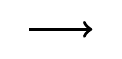
\begin{tikzpicture}
	\draw [very thick, ->] (0, 0) -- (.8,0.);
	\end{tikzpicture}
\end{textblock*}

\begin{textblock*}{5cm}(10.cm,4.4cm)
	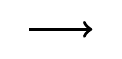
\begin{tikzpicture}
	\draw [very thick, ->] (0, 0) -- (.8,0.);
	\end{tikzpicture}
\end{textblock*}

\begin{textblock*}{5cm}(3.5cm,4.4cm)
	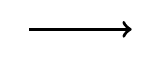
\begin{tikzpicture}
	\draw [very thick, ->] (0, 0) -- (1.3,0.);
	\end{tikzpicture}
\end{textblock*}

\begin{textblock*}{5cm}(12.cm,6.cm)
	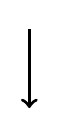
\begin{tikzpicture}
	\draw [very thick, ->] (0, 0) -- (.,-1.);
	\end{tikzpicture}
\end{textblock*}

\transfade[duration=.4]

\end{frame}

%------------------------------------------------

\subsection{NN formula}

\begin{frame}
\myframetitle{0.3\paperwidth}{0.04\paperwidth}{\insertsection}
\myframesubtitle{0.32\paperwidth}{\insertsubsection}

\centering
\includegraphics[width=1.0\linewidth]{nn_formula.png}

\end{frame}

%------------------------------------------------

\subsection{calculating weights: slide 1}

\begin{frame}
\myframetitle{0.3\paperwidth}{0.04\paperwidth}{\insertsection}
\myframesubtitle{0.32\paperwidth}{\insertsubsection}

\centering
\vspace{0.15\paperheight}
\includegraphics[width=0.35\linewidth]{perceptron_model.png}\\
\href{https://towardsdatascience.com/what-is-a-perceptron-210a50190c3b}{\color{blue}\ul{Source}}\\
\vspace{0.02\paperheight}
$Q \big(y_{model}, y_{target} \big) = Q \big(y(x, w, b), y_{target} \big)$\\
$out = y = \sigma \big(sum \big)= \sigma \big(\sum \limits_{i=1}^{3}(x_i \cdot w_i) + b \big)$
$\cfrac{\partial Q}{\partial w_i} = \cfrac{\partial Q}{\partial y} \cdot \cfrac{\partial y}{\partial \sigma} \cdot \cfrac{\partial \sigma}{\partial sum} \cdot \cfrac{\partial sum}{\partial w_i} = \cfrac{\partial Q}{\partial y} \cdot \color{red} 1 \color{black} \cdot \cfrac{\partial \sigma}{\partial sum} \cdot \cfrac{\partial sum}{\partial w_i}$\\
$\cfrac{\partial \sigma}{\partial sum} = \sigma (sum) \cdot \big(1 - \sigma (sum) \big)$

\end{frame}

%------------------------------------------------

\subsection{calculating weights: slide 2}

\begin{frame}
\myframetitle{0.3\paperwidth}{0.04\paperwidth}{\insertsection}
\myframesubtitle{0.32\paperwidth}{\insertsubsection}

\centering
\vspace{0.25\paperheight}
\begin{columns}[T]
    \column{0.5\textwidth}
    \begin{minipage}[t]{\linewidth}
        \centering
        $Q \big(y(x, w, b), y_{target} \big)$\\
        $Q = \big(y_{target} - y(x_1, w_1, b) \big)^2$\\
        $out = y = (x \cdot w) + b$\\
        $\cfrac{\partial Q}{\partial w_i} = \cfrac{\partial Q}{\partial y} \cdot \cfrac{\partial y}{\partial w_i}$\\
        Input: x = 1, w = 0.1 and b = 1\\
        $y_{target} = 2$ and learning rate: $\eta = 0.1$\\
        \onslide<2->{\color{blue} How to find $w_{new}$ and $b_{new}$? \color{black}}
    \end{minipage}
	\column{0.5\textwidth}
    \begin{minipage}[t]{\linewidth}
        \centering
        \onslide<2->{$\cfrac{\partial Q}{\partial y} = -2 \cdot (y_{target} - y)$\\
        $\cfrac{\partial Q}{\partial w} = \cfrac{\partial Q}{\partial y} \cdot \cfrac{\partial y}{\partial w} = -2 \cdot x \cdot (y_{target} - y)$\\
        $\cfrac{\partial Q}{\partial b} = \cfrac{\partial Q}{\partial y} \cdot \cfrac{\partial y}{\partial b} = -2 \cdot (y_{target} - y)$\\
        $ \color{blue} [w_{new}, b_{new}] \color{black} \Rightarrow \theta_{i+1} = \theta_i - \eta \cdot \cfrac{\partial Q(\theta_i)}{\partial \theta_i}$\\}
    \end{minipage}
\end{columns}
\hfill \break
\hfill \break
\onslide<3->{\begin{tabular}{ |p{1cm}|p{1cm}|p{1cm}|p{1cm}|p{1cm}|p{1cm}|p{1cm}| }
                \hline
                y & Q & $\cfrac{\partial Q}{\partial y}$ & $\cfrac{\partial Q}{\partial w}$ &  $\cfrac{\partial Q}{\partial b}$ & $w_{new}$ & $b_{new}$\\
                \hline
                1.1 & 0.81 & -1.8 & -1.8 & -1.8 & 0.28 & 1.18\\
                \hline
            \end{tabular}}

\end{frame}

%----------------------------------------------------------------------

\subsection{overtraining: slide 1}

\begin{frame}
\myframetitle{0.3\paperwidth}{0.04\paperwidth}{\insertsection}
\myframesubtitle{0.32\paperwidth}{\insertsubsection}

\centering
\vspace{0.2\paperheight}
\includegraphics[width=0.45\linewidth]{overtraining1.png}

\end{frame}

%------------------------------------------------

\subsection{overtraining: slide 2}

\begin{frame}
\myframetitle{0.3\paperwidth}{0.04\paperwidth}{\insertsection}
\myframesubtitle{0.32\paperwidth}{\insertsubsection}

\centering
\vspace{0.2\paperheight}
\includegraphics[width=1.0\linewidth]{overtraining2.png}

\end{frame}

%------------------------------------------------

\subsection{overtraining: slide 3}

\begin{frame}
\myframetitle{0.3\paperwidth}{0.04\paperwidth}{\insertsection}
\myframesubtitle{0.32\paperwidth}{\insertsubsection}

\centering
\vspace{0.05\paperheight}
\includegraphics[width=1.0\linewidth]{overtraining3.png}

\end{frame}

%------------------------------------------------

\subsection{overtraining: slide 4}

\begin{frame}
\myframetitle{0.3\paperwidth}{0.04\paperwidth}{\insertsection}
\myframesubtitle{0.32\paperwidth}{\insertsubsection}

\centering
\vspace{0.15\paperheight}
\includegraphics[width=0.7\linewidth]{tanks_history.png}

\end{frame}

%------------------------------------------------

\subsection{Math and ML}

\begin{frame}
\myframetitle{0.3\paperwidth}{0.04\paperwidth}{\insertsection}
\myframesubtitle{0.32\paperwidth}{\insertsubsection}

\vspace{0.2\paperheight}
\begin{columns}
    \centering
	\column{0.5\textwidth}
	\begin{minipage}[t]{\linewidth}
	    \includegraphics[width=1.0\linewidth]{import_keras.png}
    \end{minipage}%
    \column{0.5\textwidth}
    \begin{minipage}[t]{\linewidth}
        \centering
    	\includegraphics[width=1.0\linewidth]{ml_newbie.png}
    \end{minipage}
\end{columns}

\end{frame}

%------------------------------------------------

\subsection{The Toolkit for Multivariate Analysis (TMVA)}

\begin{frame}
\myframetitle{0.3\paperwidth}{0.04\paperwidth}{\insertsection}
\myframesubtitle{0.32\paperwidth}{\insertsubsection}

\centering
\vspace{0.2\paperheight}

TMVA is the ROOT library that provides the interfaces and implementations of the above mentioned machine learning techniques. The package includes:

\begin{itemize}
	\setbeamertemplate{items}{\mybullet}
	\item {Neural networks}
	\item {Deep networks}
	\item {Boosted/Bagged decision trees}
	\item {Multidimensional k-nearest neighbour classifier}
	\item {Support Vector Machine (SVM)}
	\item {...}
\end{itemize}

\href{https://root.cern/manual/tmva/}{\color{blue}\ul{https://root.cern/manual/tmva/}}

\end{frame}

%------------------------------------------------

\subsection{TMVA 1}

\begin{frame}
\myframetitle{0.3\paperwidth}{0.04\paperwidth}{\insertsection}
\myframesubtitle{0.32\paperwidth}{\insertsubsection}

\vspace{0.2\paperheight}
\centering
	\includegraphics[width=0.9\linewidth]{tmva1.png}

\end{frame}

%------------------------------------------------

\subsection{TMVA 2}

\begin{frame}
\myframetitle{0.3\paperwidth}{0.04\paperwidth}{\insertsection}
\myframesubtitle{0.32\paperwidth}{\insertsubsection}

\vspace{0.2\paperheight}
\centering
	\includegraphics[width=0.9\linewidth]{tmva2.png}

\end{frame}

%------------------------------------------------

\subsection{TMVA 3}

\begin{frame}
\myframetitle{0.3\paperwidth}{0.04\paperwidth}{\insertsection}
\myframesubtitle{0.32\paperwidth}{\insertsubsection}

\vspace{0.2\paperheight}
\centering
	\includegraphics[width=0.9\linewidth]{tmva3.png}

\end{frame}

%------------------------------------------------

\subsection{XGBoost}

\begin{frame}
\myframetitle{0.3\paperwidth}{0.04\paperwidth}{\insertsection}
\myframesubtitle{0.32\paperwidth}{\insertsubsection}

\vspace{0.2\paperheight}
\centering
	\includegraphics[width=1\linewidth]{xgboost.png}

\end{frame}

%------------------------------------------------

\subsection{Keras 1}

\begin{frame}
\myframetitle{0.3\paperwidth}{0.04\paperwidth}{\insertsection}
\myframesubtitle{0.32\paperwidth}{\insertsubsection}

\vspace{0.2\paperheight}
\centering
	\includegraphics[width=0.85\linewidth]{keras1.png}

\end{frame}

%------------------------------------------------

\subsection{Keras 2}

\begin{frame}
\myframetitle{0.3\paperwidth}{0.04\paperwidth}{\insertsection}
\myframesubtitle{0.32\paperwidth}{\insertsubsection}

\vspace{0.2\paperheight}
\centering
	\includegraphics[width=0.5\linewidth]{keras2.png}

\end{frame}

%------------------------------------------------

\subsection{Keras 3}

\begin{frame}
\myframetitle{0.3\paperwidth}{0.04\paperwidth}{\insertsection}
\myframesubtitle{0.32\paperwidth}{\insertsubsection}

\vspace{0.2\paperheight}
\centering
	\includegraphics[width=0.65\linewidth]{keras3.png}

\end{frame}

%------------------------------------------------

\backupend

\end{document}
